%% History:
% Pavel Tvrdik (26.12.2004)
%  + initial version for PhD Report
%
% Daniel Sykora (27.01.2005)
%
% Michal Valenta (3.12.2008)
% rada zmen ve formatovani (diky M. Duškovi, J. Holubovi a J. Žďárkovi)
% sjednoceni zdrojoveho kodu pro anglickou, ceskou, bakalarskou a diplomovou praci

% One-page layout: (proof-)reading on display
%%%% \documentclass[11pt,oneside,a4paper]{book}
% Two-page layout: final printing
\documentclass[11pt,twoside,a4paper]{book}   

\usepackage{wrapfig, floatrow, amsmath, url, graphicx, array, breakurl}
%\usepackage[breaklinks]{hyperref}

\usepackage[czech, english]{babel}
\usepackage[T1]{fontenc} % pouzije EC fonty 
% pripadne pisete-li cesky, pak lze zkusit take:
% \usepackage[OT1]{fontenc} 
\usepackage[utf8]{inputenc}
%=-=-=-=-=-=-=-=-=-=-=-=--=%
% In case of problems with PDF fonts, one may try to uncomment this line:
%\usepackage{lmodern}
%=-=-=-=-=-=-=-=-=-=-=-=--=%
%=-=-=-=-=-=-=-=-=-=-=-=--=%
% Depending on your particular TeX distribution and version of conversion tools 
% (dvips/dvipdf/ps2pdf), some (advanced | desperate) users may prefer to use 
% different settings.
% Please uncomment the following style and use your CSLaTeX (cslatex/pdfcslatex) 
% to process your work. Note however, this file is in UTF-8 and a conversion to 
% your native encoding may be required. Some settings below depend on babel 
% macros and should also be modified. See \selectlanguage \iflanguage.
%\usepackage{czech}  %%%%%\usepackage[T1]{czech} %%%%[IL2] [T1] [OT1]
%=-=-=-=-=-=-=-=-=-=-=-=--=%

%%%%%%%%%%%%%%%%%%%%%%%%%%%%%%%%%%%%%%%
% Styles required in your work follow %
%%%%%%%%%%%%%%%%%%%%%%%%%%%%%%%%%%%%%%%
\usepackage{graphicx}
\usepackage{indentfirst} %1. odstavec jako v cestine.
\usepackage{listings}
\usepackage{color}
\usepackage{soul}
\setul{0.1ex}{}

\renewcommand{\lstlistingname}{Ukázka}

\definecolor{mygreen}{rgb}{0,0.6,0}
\definecolor{mygray}{rgb}{0.5,0.5,0.5}
\definecolor{mymauve}{rgb}{0.58,0,0.82}

\lstset{ %
  backgroundcolor=\color{white},   % choose the background color; you must add \usepackage{color} or \usepackage{xcolor}
  basicstyle=\footnotesize,        % the size of the fonts that are used for the code
  breakatwhitespace=false,         % sets if automatic breaks should only happen at whitespace
  breaklines=true,                 % sets automatic line breaking
  captionpos=b,                    % sets the caption-position to bottom
  commentstyle=\color{mygreen},    % comment style
  deletekeywords={...},            % if you want to delete keywords from the given language
  escapeinside={\%*}{*)},          % if you want to add LaTeX within your code
  extendedchars=true,              % lets you use non-ASCII characters; for 8-bits encodings only, does not work with UTF-8
  frame=single,                    % adds a frame around the code
  keepspaces=true,                 % keeps spaces in text, useful for keeping indentation of code (possibly needs columns=flexible)
  keywordstyle=\color{blue},       % keyword style
  language=Octave,                 % the language of the code
  morekeywords={*,...},            % if you want to add more keywords to the set
  numbers=left,                    % where to put the line-numbers; possible values are (none, left, right)
  numbersep=5pt,                   % how far the line-numbers are from the code
  numberstyle=\tiny\color{mygray}, % the style that is used for the line-numbers
  rulecolor=\color{black},         % if not set, the frame-color may be changed on line-breaks within not-black text (e.g. comments (green here))
  showspaces=false,                % show spaces everywhere adding particular underscores; it overrides 'showstringspaces'
  showstringspaces=false,          % underline spaces within strings only
  showtabs=false,                  % show tabs within strings adding particular underscores
  stepnumber=1,                    % the step between two line-numbers. If it's 1, each line will be numbered
  stringstyle=\color{mymauve},     % string literal style
  tabsize=2,                       % sets default tabsize to 2 spaces
  title=\lstname                   % show the filename of files included with \lstinputlisting; also try caption instead of title
}
\lstdefinelanguage{GLSL}
{
sensitive=true,
morekeywords=[1]{
attribute, const, uniform, varying,
layout, centroid, flat, smooth,
noperspective, break, continue, do,
for, while, switch, case, default, if,
else, in, out, inout, float, int, void,
bool, true, false, invariant, discard,
return, mat2, mat3, mat4, mat2x2, mat2x3,
mat2x4, mat3x2, mat3x3, mat3x4, mat4x2,
mat4x3, mat4x4, vec2, vec3, vec4, ivec2,
ivec3, ivec4, bvec2, bvec3, bvec4, uint,
uvec2, uvec3, uvec4, lowp, mediump, highp,
precision, sampler1D, sampler2D, sampler3D,
samplerCube, sampler1DShadow,
sampler2DShadow, samplerCubeShadow,
sampler1DArray, sampler2DArray,
sampler1DArrayShadow, sampler2DArrayShadow,
isampler1D, isampler2D, isampler3D,
isamplerCube, isampler1DArray,
isampler2DArray, usampler1D, usampler2D,
usampler3D, usamplerCube, usampler1DArray,
usampler2DArray, sampler2DRect,
sampler2DRectShadow, isampler2DRect,
usampler2DRect, samplerBuffer,
isamplerBuffer, usamplerBuffer, sampler2DMS,
isampler2DMS, usampler2DMS,
sampler2DMSArray, isampler2DMSArray,
usampler2DMSArray, struct},
morekeywords=[2]{
radians,degrees,sin,cos,tan,asin,acos,atan,
atan,sinh,cosh,tanh,asinh,acosh,atanh,pow,
exp,log,exp2,log2,sqrt,inversesqrt,abs,sign,
floor,trunc,round,roundEven,ceil,fract,mod,modf,
min,max,clamp,mix,step,smoothstep,isnan,isinf,
floatBitsToInt,floatBitsToUint,intBitsToFloat,
uintBitsToFloat,length,distance,dot,cross,
normalize,faceforward,reflect,refract,
matrixCompMult,outerProduct,transpose,
determinant,inverse,lessThan,lessThanEqual,
greaterThan,greaterThanEqual,equal,notEqual,
any,all,not,textureSize,texture,textureProj,
textureLod,textureOffset,texelFetch,
texelFetchOffset,textureProjOffset,
textureLodOffset,textureProjLod,
textureProjLodOffset,textureGrad,
textureGradOffset,textureProjGrad,
textureProjGradOffset,texture1D,texture1DProj,
texture1DProjLod,texture2D,texture2DProj,
texture2DLod,texture2DProjLod,texture3D,
texture3DProj,texture3DLod,texture3DProjLod,
textureCube,textureCubeLod,shadow1D,shadow2D,
shadow1DProj,shadow2DProj,shadow1DLod,
shadow2DLod,shadow1DProjLod,shadow2DProjLod,
dFdx,dFdy,fwidth,noise1,noise2,noise3,noise4,
EmitVertex,EndPrimitive},
morekeywords=[3]{
gl_VertexID,gl_InstanceID,gl_Position,
gl_PointSize,gl_ClipDistance,gl_PerVertex,
gl_Layer,gl_ClipVertex,gl_FragCoord,
gl_FrontFacing,gl_ClipDistance,gl_FragColor,
gl_FragData,gl_MaxDrawBuffers,gl_FragDepth,
gl_PointCoord,gl_PrimitiveID,
gl_MaxVertexAttribs,gl_MaxVertexUniformComponents,
gl_MaxVaryingFloats,gl_MaxVaryingComponents,
gl_MaxVertexOutputComponents,
gl_MaxGeometryInputComponents,
gl_MaxGeometryOutputComponents,
gl_MaxFragmentInputComponents,
gl_MaxVertexTextureImageUnits,
gl_MaxCombinedTextureImageUnits,
gl_MaxTextureImageUnits,
gl_MaxFragmentUniformComponents,
gl_MaxDrawBuffers,gl_MaxClipDistances,
gl_MaxGeometryTextureImageUnits,
gl_MaxGeometryOutputVertices,
gl_MaxGeometryOutputVertices,
gl_MaxGeometryTotalOutputComponents,
gl_MaxGeometryUniformComponents,
gl_MaxGeometryVaryingComponents,gl_DepthRange},
morecomment=[l]{//},
morecomment=[s]{/*}{*/},
morecomment=[l][keywordstyle4]{\#},
} 
 
\usepackage{k336_thesis_macros} % specialni makra pro formatovani DP a BP
 % muzete si vytvorit i sva vlastni v souboru k336_thesis_macros.sty
 % najdete  radu jednoduchych definic, ktere zde ani nejsou pouzity
 % napriklad: 
 % \newcommand{\bfig}{\begin{figure}\begin{center}}
 % \newcommand{\efig}{\end{center}\end{figure}}
 % umoznuje pouzit prikaz \bfig namisto \begin{figure}\begin{center} atd.


\newcommand\TypeOfWork{Diplomová práce} \typeout{Diplomova prace}
\newcommand\StudProgram{Otevřená informatika, Navazující magisterský}
\newcommand\StudBranch{Počítačová grafika a interakce}
\newcommand\WorkTitle{Zobrazování rozsáhlých scén s předpočteným osvětlením}
\newcommand\FirstandFamilyName{Bc. Luboš Vonásek}
\newcommand\Supervisor{Ing. Jiří Bittner, Ph.D.}


% Pouzijete-li pdflatex, tak je prijemne, kdyz bude mit vase prace
% funkcni odkazy i v pdf formatu
\usepackage[
pdftitle={\WorkTitle},
pdfauthor={\FirstandFamilyName},
bookmarks=true,
colorlinks=true,
breaklinks=true,
urlcolor=black,
citecolor=blue,
linkcolor=blue,
unicode=true,
]
{hyperref}




\begin{document}

%%%%%%%%%%%%%%%%%%%%%%%%%%%%%%%%%%%%%
% Zvolte jednu z moznosti 
% Choose one of the following options
%%%%%%%%%%%%%%%%%%%%%%%%%%%%%%%%%%%%%
\selectlanguage{czech}
%\selectlanguage{english} 

% prikaz \typeout vypise vyse uvedena nastaveni v prikazovem okne
% pro pohodlne ladeni prace


\iflanguage{czech}{
	 \typeout{************************************************}
	 \typeout{Zvoleny jazyk: cestina}
	 \typeout{Typ prace: \TypeOfWork}
	 \typeout{Studijni program: \StudProgram}
	 \typeout{Obor: \StudBranch}
	 \typeout{Jmeno: \FirstandFamilyName}
	 \typeout{Nazev prace: \WorkTitle}
	 \typeout{Vedouci prace: \Supervisor}
	 \typeout{***************************************************}
	 \newcommand\Department{Katedra počítačové grafiky a interakce}
	 \newcommand\Faculty{Fakulta elektrotechnická}
	 \newcommand\University{České vysoké učení technické v Praze}
	 \newcommand\labelSupervisor{Vedoucí práce}
	 \newcommand\labelStudProgram{Studijní program}
	 \newcommand\labelStudBranch{Obor}
}{
	 \typeout{************************************************}
	 \typeout{Language: english}
	 \typeout{Type of Work: \TypeOfWork}
	 \typeout{Study Program: \StudProgram}
	 \typeout{Study Branch: \StudBranch}
	 \typeout{Author: \FirstandFamilyName}
	 \typeout{Title: \WorkTitle}
	 \typeout{Supervisor: \Supervisor}
	 \typeout{***************************************************}
	 \newcommand\Department{Department of Computer Graphics and Interaction}
	 \newcommand\Faculty{Faculty of Electrical Engineering}
	 \newcommand\University{Czech Technical University in Prague}
	 \newcommand\labelSupervisor{Supervisor}
	 \newcommand\labelStudProgram{Study Programme} 
	 \newcommand\labelStudBranch{Field of Study}
}




%%%%%%%%%%%%%%%%%%%%%%%%%%    Poznamky ke kompletaci prace
% Nasledujici pasaz uzavrenou v {} ve sve praci samozrejme 
% zakomentujte nebo odstrante. 
% Ve vysledne svazane praci bude nahrazena skutecnym 
% oficialnim zadanim vasi prace.
{
\pagenumbering{roman} \cleardoublepage \thispagestyle{empty}
\chapter*{Na tomto místě bude oficiální zadání vaší práce}
\begin{itemize}
\item Toto zadání je podepsané děkanem a vedoucím katedry,
\item musíte si ho vyzvednout na studiijním oddělení Katedry počítačů na Karlově náměstí,
\item v jedné odevzdané práci bude originál tohoto zadání (originál zůstává po obhajobě na katedře),
\item ve druhé bude na stejném místě neověřená kopie tohoto dokumentu (tato se vám vrátí po obhajobě).
\end{itemize}
}
%to print missing literature in reference
\cite{Fast03} \cite{OpenGL10} \cite{Hawkins01} \cite{Buss03} \cite{Ericson04} \cite{Modern04}
\newpage

%%%%%%%%%%%%%%%%%%%%%%%%%%    Titulni stranka / Title page 
\coverpagestarts

%%%%%%%%%%%%%%%%%%%%%%%%%%%    Podekovani / Acknowledgements 
\acknowledgements
\noindent
Rád bych poděkoval panu Jiřímu Bittnerovi za vedení této diplomové práce, za obrovské množství užitečných rad a za připomínky, které mi pomohly zvýšit kvalitu práce. Dále bych rád poděkoval učitelům z katedry počítačové grafiky a interakce za kvalitní výuku a za mnoho předaných znalostí, které jsem v této práci využil.


%%%%%%%%%%%%%%%%%%%%%%%%%%%   Prohlaseni / Declaration 
\declaration{V~Praze dne 12.\,5.\,2014}


%%%%%%%%%%%%%%%%%%%%%%%%%%%%    Abstract 
\abstractpage
The goal of this Masters thesis is rendering large scenes with precomputed illumination on smartphones. Precomputed illumination is generated using rasterisation or raycasting. Results are stored as lightmaps. Lightmaps are dynamically updated by patches depending on the change of light sources. Precomputed illumination is also applied to dynamic objects in the scene. The project is written in C++ and uses the OpenGL library. The thesis contains testing of performance and memory consumption at different levels of detail. The thesis also contains performance comparation of laptop, tablet a smartphone.
% Prace v cestine musi krome abstraktu v anglictine obsahovat i
% abstrakt v cestine.
\vglue60mm

\noindent{\Huge \textbf{Abstrakt}}
\vskip 2.75\baselineskip

\noindent
Cílem této diplomové práce je zobrazování rozsáhlých scén s předpočteným osvětlením\linebreak na mobilních zařízeních. Předpočtené osvětlení je generováno pomocí rasterizace nebo vrhání paprsků. Výsledky jsou ukládány ve formě map osvětlení. Mapy osvětlení jsou dynamicky aktualizovány pomocí záplat v závislosti na změně stavu světel. Předpočtené osvětlení je také aplikováno na dynamické objekty ve scéně. Projekt je psaný v jazyce C++ a používá knihovnu OpenGL. Práce obsahuje testování výpočetní a paměťové náročnosti při různých úrovních detailu. Práce také obsahuje porovnání výkonu notebooku, tabletu a mobilního zařízení.


%%%%%%%%%%%%%%%%%%%%%%%%%%%%%%%%  Obsah / Table of Contents 
\tableofcontents


%%%%%%%%%%%%%%%%%%%%%%%%%%%%%%%  Seznam obrazku / List of Figures 
\listoffigures


%%%%%%%%%%%%%%%%%%%%%%%%%%%%%%%  Seznam tabulek / List of Tables
\listoftables


%**************************************************************
\mainbodystarts
% horizontalní mezera mezi dvema odstavci
%\parskip=5pt
%11.12.2008 parskip + tolerance
\normalfont
\parskip=0.2\baselineskip plus 0.2\baselineskip minus 0.1\baselineskip

% Odsazeni prvniho radku odstavce resi class book (neaplikuje se na prvni 
% odstavce kapitol, sekci, podsekci atd.) Viz usepackage{indentfirst}.
% Chcete-li selektivne zamezit odsazeni 1. radku nektereho odstavce,
% pouzijte prikaz \noindent.

%**************************************************************

% Pro snadnejsi praci s vetsimi texty je rozumne tyto rozdelit
% do samostatnych souboru nejlepe dle kapitol a tyto potom vkladat
% pomoci prikazu \include{jmeno_souboru.tex} nebo \include{jmeno_souboru}.
% Napr.:
% \include{1_uvod}
% \include{2_teorie}
% atd...

%*****************************************************************************
\chapter{Úvod}
Za posledních deset let se výkon hardwaru mobilních zařízeních několikanásobně zvýšil. Mobilní zařízení disponují procesory s více jádry, grafickou kartu umožňující paralelizaci grafických výpočtů a mají gigabajty operační paměti. 

Kromě vylepšování hardwaru se vylepšují také metody pro optimalizaci výpočtu, jedna z těchto metod je předpočtení dat. Tato práce se zabývá předpočtením dat pro vykreslování scény nočního města. Scéna obsahuje jak bodové, tak plošné zdroje světla, pro které by výpočet v reálném čase byl příliš náročný. 

Práce obsahuje přehled souvisejících metod zabývajících se vykreslováním noční scény, utváří přehled teorie výpočtu osvětlení a doplňujících grafických efektů. Rozebírá tématiku předpočteného osvětlení, zaměřuje se na řešení dílčích problémů předpočteného osvětlení. Následuje popis implementace použité metody, která řeší také dynamické aktualizování osvětlení.

Na závěr práce je provedeno testování aplikace pro předpočtení osvětlení a testovací aplikace, která zobrazuje výsledky práce. Je zde provedena stručná diskuze nad výsledky testování a shrnutí celkových výsledků. 

%*****************************************************************************
\chapter{Specifikace práce}
Cílem práce bylo realizovat efektivní vykreslování rozsáhlých nočních scén na platformě Android za použití grafické knihovny OpenGL. Rozhodl jsem se aplikaci realizovat v podobě závodního simulátoru, jehož scéna je noční město obsahující několik pohybujících se vozidel, několik zhasínajících světel a řádově desetitisíce statických zdrojů světel. Statická světla jsou předpočtená pomocí map osvětlení (anglicky lightmap), mapy osvětlení jsou textury 3D modelů, které obsahují informace o difúzní složce osvětlovacího modelu. Difúzní složka je závislá pouze na poloze světla, směru světla a povrchu tělesa, lze jí tedy pro statickou část modelu předpočítat.

Důraz byl kladen na co nejvyšší optimalizaci vykreslování. Kromě hlavní grafické techniky map osvětlení bylo použito několik dalších technik řešící jednotlivé problémy, které vznikají při použití map osvětlení. Problematické je použití dynamických objektů a dynamická aktualizace osvětlení. Technika map osvětlení řeší pouze statickou scénu a v případě použití dynamické scény bylo potřeba metodu značně rozšířit.

\section{Požadavky na funkčnost}
Zadání předpokládá, že projekt bude rozdělen do dvou samostatných částí. První částí bude předzpracování, ve kterém se budou vytvářet mapy osvětlení. Druhou částí projektu bude aplikace, která mapy osvětlení využije. Fázi předzpracování by teoreticky bylo možné provádět i na platformě Android. Vzhledem k tomu, že klasické počítače dosahují vyššího výkonu než mobilní zařízení, bude efektivnější provést předzpracování na stolním počítači.

Metoda bude navržena tak, aby bylo umožněno některá světla v reálném čase zhasínat\linebreak a znovu rozsvěcovat nezávisle na sobě. Veškerá bodová světla budou vrhat spekulární odlesky na dynamické objekty.

Předpočtené osvětlení bude využívat dva formáty dat - rastrový a vektorový. Rastrový bude určen pro statické osvětlení scény a vektorové pro dynamická světla. Využití plochy map osvětlení bude maximalizováno z důvodu očekávané malé paměti vymezené pro velké textury. Aby bylo možné určit nejvhodnější rozlišení těchto textur, bude umožněno škálování map osvětlení.

\subsection{Statické osvětlení s dynamickými objekty ve scéně}
Při použití dynamických objektů ve scéně se statickém osvětlením vznikají dva základní problémy. Prvním problém je, že dynamické objekty mají jiné osvětlení než statická scéna\linebreak a to vypadá velice nepřirozeně. Druhým problémem je, že pokud dynamický objekt zastíní zdroj světla, tak nevznikne stín na statických objektech.

Oba problémy lze vyřešit jen částečně. V prvním případě se bude číst informace o intenzitě osvětlení z nejbližšího bodu na statickém objektu a tato intenzita se bude aplikovat na dynamický objekt. V druhém případě při vykreslování jednotlivých pixelů se bude zjišťovat, zda se v okolí vykreslovaného bodu nenachází dynamický objekt a podle toho se bude aplikovat zastínění.

\section{Cílová platforma Android}
Platforma Android je postavena na Linuxovém jádře a využívá knihovny, které bývají součástí unixových systémů. Od klasického desktopového Linuxu se odlišuje hlavně v tom, že jako hlavní programovací jazyk využívá Javu. Pomocí Javy je naprogramováno celé Android API, které zprostředkovává téměř veškeré služby systému.

Pro platformu Android existuje nepřeberné množství aplikací a toho začínají využívat ostatní platformy. V současné době platformy BlackBerry a Jolla umožňují spouštět Android aplikace. Dále existuje platforma NokiaX, která je postavena přímo na operačním systému Android.

\section{Související metody}

Rešerši souvisejících metod jsem zaměřil na dvě různé kategorie. První kategorie jsou implementace pro PC, kde je nejčastěji řešeno nepřímé osvětlení, které by pro mobilní zařízení bylo příliš náročné na výpočet. Druhá kategorie jsou závodní simulátory s noční jízdou pro platformu Android. V této kategorii bývají nejčastěji použity techniky jako v této práci.

\subsection{Vykreslování noční scény}

V této sekci jsem vybral co nejrealističtější implementace, ke kterým existuje článek o tom, jak bylo výsledku dosaženo. Existuje sice několik implementací, které vypadají realističtěji. To jsou ale většinou komerční produkty, které nesdílejí ostatním, jakým způsobem byla implementace realizována.

\paragraph{Interaktivní vykreslování modelů měst s globálním osvětlením}\mbox{}\\

Interaktivní vykreslování modelů měst\cite{Interact12} je technika založená na fotonovém mapování, která používá 2D buffery pro uložení fotonové energie jdoucí směrem k povrchu modelu. Tyto buffery jsou namapovány na neviditelné válce, které umožňují rychle vypočítat globální osvětlení v jeho okolí.

Metoda umožňuje zobrazování zrcadlových odlesků, ostrých stínů a umožňuje aktualizovat předpočtenou informaci za běhu aplikace. Projekt je specifický tím, že umožňuje vykreslovat rozsáhle scény s globálním osvětlením v reálném čase. 

Autoři projektu neuvádí použitelnost metody s noční scénou. Pravděpodobně by při použití noční scény nastal problém s aktualizováním fotonových map.

\begin{center}
\begin{figure}[h!]
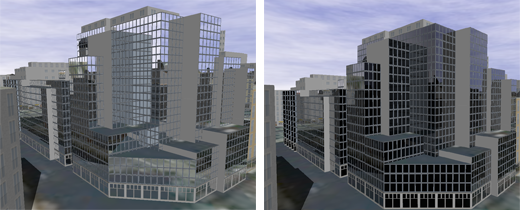
\includegraphics[width=100mm]{figures/PM.png}
\caption{Ukázka vykreslené scény pomocí fotonového mapování \cite{Interact12}}
\end{figure}
\end{center}


\paragraph{Proceduralní modelování města a osvětlení nočního města}\mbox{}\\

Projekt \uv{Proceduralní modelování města a osvětlení nočního města}\cite{Chen99} byl představen roku 1999 a zabývá se proceduálním modelováním města (konkrétně Bostonu), který je vykreslován pomocí sledování paprsku za využití metody Monte Carlo. Metoda pro každý bod na obrazovce nalezne odpovídající 3D bod v prostoru, z něj vyšle několik náhodných paprsků a vyhodnotí výsledné osvětlení.

Implementace neběží v reálném čase. Výsledek je při detailním záběru po grafické stránce velice realistický. Reflektory vozidla osvětlují pouze blízké okolí. Při záběru\linebreak na město z výšky výsledek nebudí tolik realistický dojem jako při detailním záběru.

\begin{center}
\begin{figure}[h!]
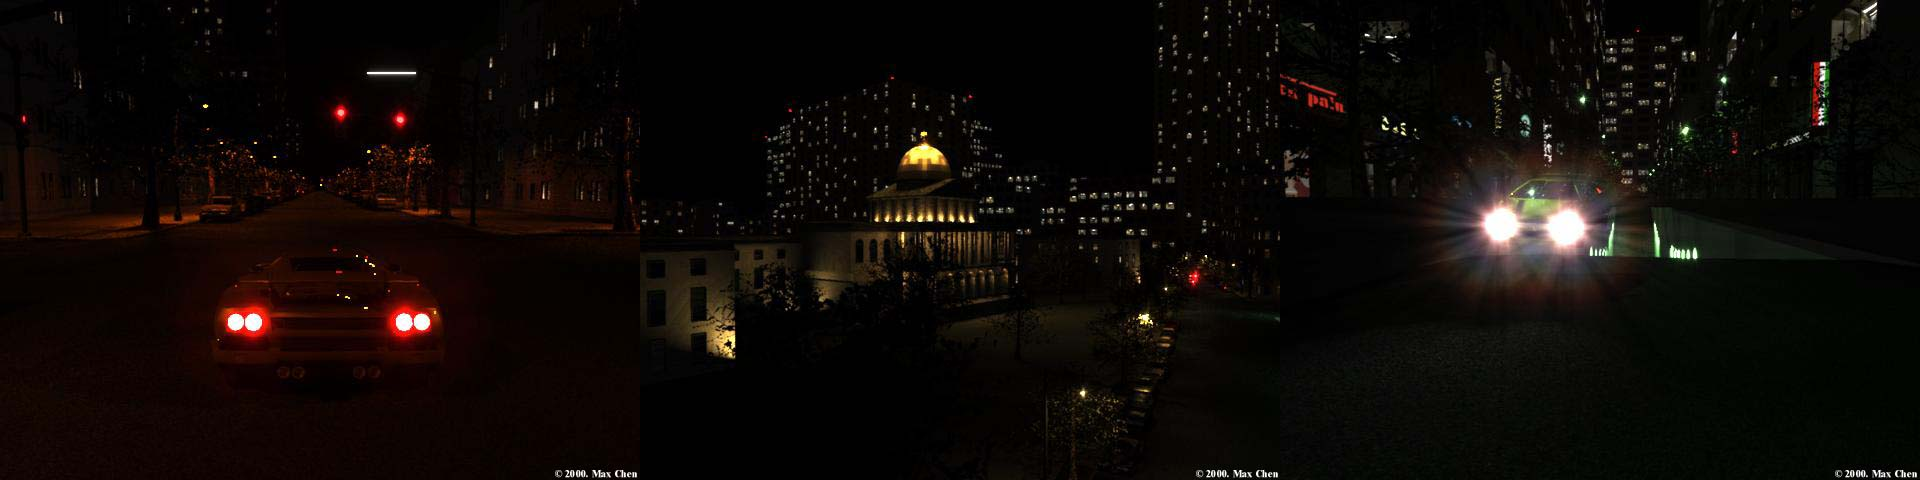
\includegraphics[width=150mm]{figures/NR.png}
\caption{Ukázka nočního renderingu \cite{Chen99}}
\end{figure}
\end{center}
\newpage

\paragraph{Imperfect shadow maps pro výpočet nepřímého osvětlení}\mbox{}\\

Technika imperfect shadow maps\cite{Ritschel:2008:ISM}, představená roku 2008, se nezabývá přímo noční scénou, zabývá se nepřímým osvětlením, které s noční scénou souvisí. Implementace běží\linebreak v reálném čase a její výsledky jsou srovnatelné se snímky, které se vykreslují několik hodin.

V této implementaci se nevyužívá předpočtených dat. Využívá se zde virtuálních bodových světel (VPL) převzorkovaných do bodů ve scéně, která simulují odrazy světla.\linebreak Z každého VPL se vytvoří stínová mapa o malém rozlišení a při vykreslování výsledné scény se vyhodnocuje viditelnost ze všech VPL.

Implementace podporuje více typů zdrojů světla, včetně plošných. Nemá problémy\linebreak s barevným světlem ani s kaustiky.

\begin{figure}[h!]
\begin{center}
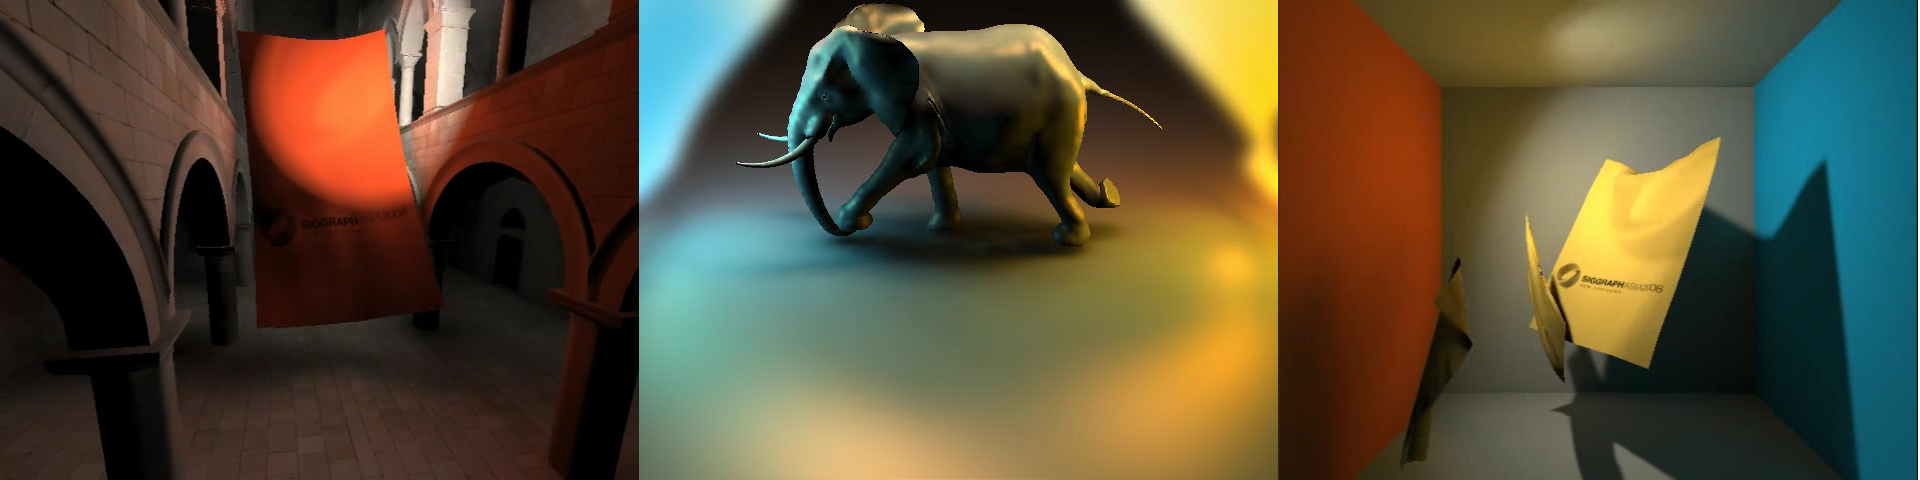
\includegraphics[width=150mm]{figures/ISM.png}
\caption{Ukázka výsledků techniky imperfektních stínových map pro efektivní výpočet nepřímého osvětlení \cite{Ritschel:2008:ISM}}
\end{center}
\end{figure}

\subsection{Závodní simulátory s noční scénou pro platformu Android}
V této sekci jsem vyhledával i implementace, u kterých není uvedeno, jak bylo výsledků dosaženo. Je to z důvodu malého počtu implementací odpovídající dané kategorii.

\paragraph{Asphalt Urban}\mbox{}\\

Asphalt Urban je série mobilních závodních simulátorů, jejíchž první díl byl publikován spolu s herním smartphonem Nokia N-Gage. Jedná se o úspěšnou sérii, která přitahuje hráče všech možných platforem.

Zmíním 7.díl ze série Asphalt Urban, který osobně považuji za nejúspěšnější díl. Osvětlení z pouličních lamp je součástí textur, reflektor vozidla je tvořen zřejmě pomocí projektivní textury. Povrch zrcadlově odráží 3D objekty. Po bližším zkoumání lze zjistit, že některé tyto odražené objekty jsou odlišné. Domnívám se, že zde byl použit duplicitní objekt.

Další díl ze série Asphalt Urban už odlesky řeší lépe. Odráží se hlavně světla a odlesk je lépe přizpůsoben povrchu. Vzniká zde dojem mokré silnice. Dochází i k rozmazání brzdových světel. Osvětlení od lamp je opět řešeno texturou. Nepříjemnou změnou je absence reflektoru vozidla a přidání rušivého chvění kamery během jízdy.

\paragraph{Need for Speed Most Wanted}\mbox{}\\

V tomto simulátoru je osvětlení řešeno hlavně konstantním osvětlením pro celou scénu, pouliční lampy využívají bilboardů a neosvětlují okolí. Výrazný je odraz světla na vozovce v kombinaci s bump mapováním vytváří dojem hrubého povrchu.

Simulátor je spíše známý z PC, na mobilním trhu takový úspěch nemá. Od PC verze je velice odlišný, ale rozhodně se nejedná o nějakou lacinou napodobeninu. Jedná se o první závodní simulátor pro mobilní zařízení, který disponuje modelem ničení vozidla (je možné vozidlo poškrábat, rozbít mu okna apod).

Oproti Asphalt 8 má navíc efekt Depth-of-field. To znamená, že vzdálené modely jsou rozmazané a zabarveny do barvy pozadí. Tento efekt vytváří příjemný mlhovitý dojem. Jinak bych řekl, že tyto dva simulátory jsou si sobě velice podobné. Na stejném enginu funguje\linebreak i známý simulátor Real Racing 3, který noční jízdou nedisponuje.

\paragraph{GT Racing 2}\mbox{}\\

Úspěšným závodním simulátorem je v současné době GT Racing 2, je to hlavně díky jeho zpracování. Jako jediný z uvedených simulátorů má při noční jízdě nízké ambientní osvětlení a scéna je osvětlena hlavně reflektorem vozidla.

Osvětlení lampami je pravděpodobně přímo součástí textur, použití map osvětlení by bylo pro použité 3D modely příliš náročné.

\paragraph{Sports Car Challenge}\mbox{}\\

Noční jízda je v tomto projektu realizována stejnými technikami jako denní jízda. Jsou zde použity pouze tmavé textury a halo efekt pouličních lamp.

Simulátor disponuje asi nejdetailnějšími modely vozidel. Vývojář spolupracuje s předními výrobci automobilů a to se odrazilo právě na modelech vozidel. Modely jsou realistické a to včetně interiérů. Projekt trpí slabší kompatibilitou s mobilními zařízeními, i když náročnost enginu je nízká.

\paragraph{Track Racing}\mbox{}\\

I když tento projekt není závodní simulátor s noční jízdou, zmiňuji ho hlavně kvůli ovládání. Jedná se o neoficiální remake hry Trackmania známé z PC. Projekt běží na Unity3D enginu a je dostupný na mnoha platformách, nedá se ale stáhnout přímo z Marketu či Storu.

U výše uvedených simulátorů vozidlo automaticky zrychluje a u některých i samo brzdí. Hráč nemá tedy nad vozidlem takovou kontrolu. V případě Track Racing má hráč nad vozidlem plnou kontrolu a zážitek ze hry se dá srovnat se zážitkem z původní PC hry.
\newpage

\begin{center}
\begin{figure}[h!]
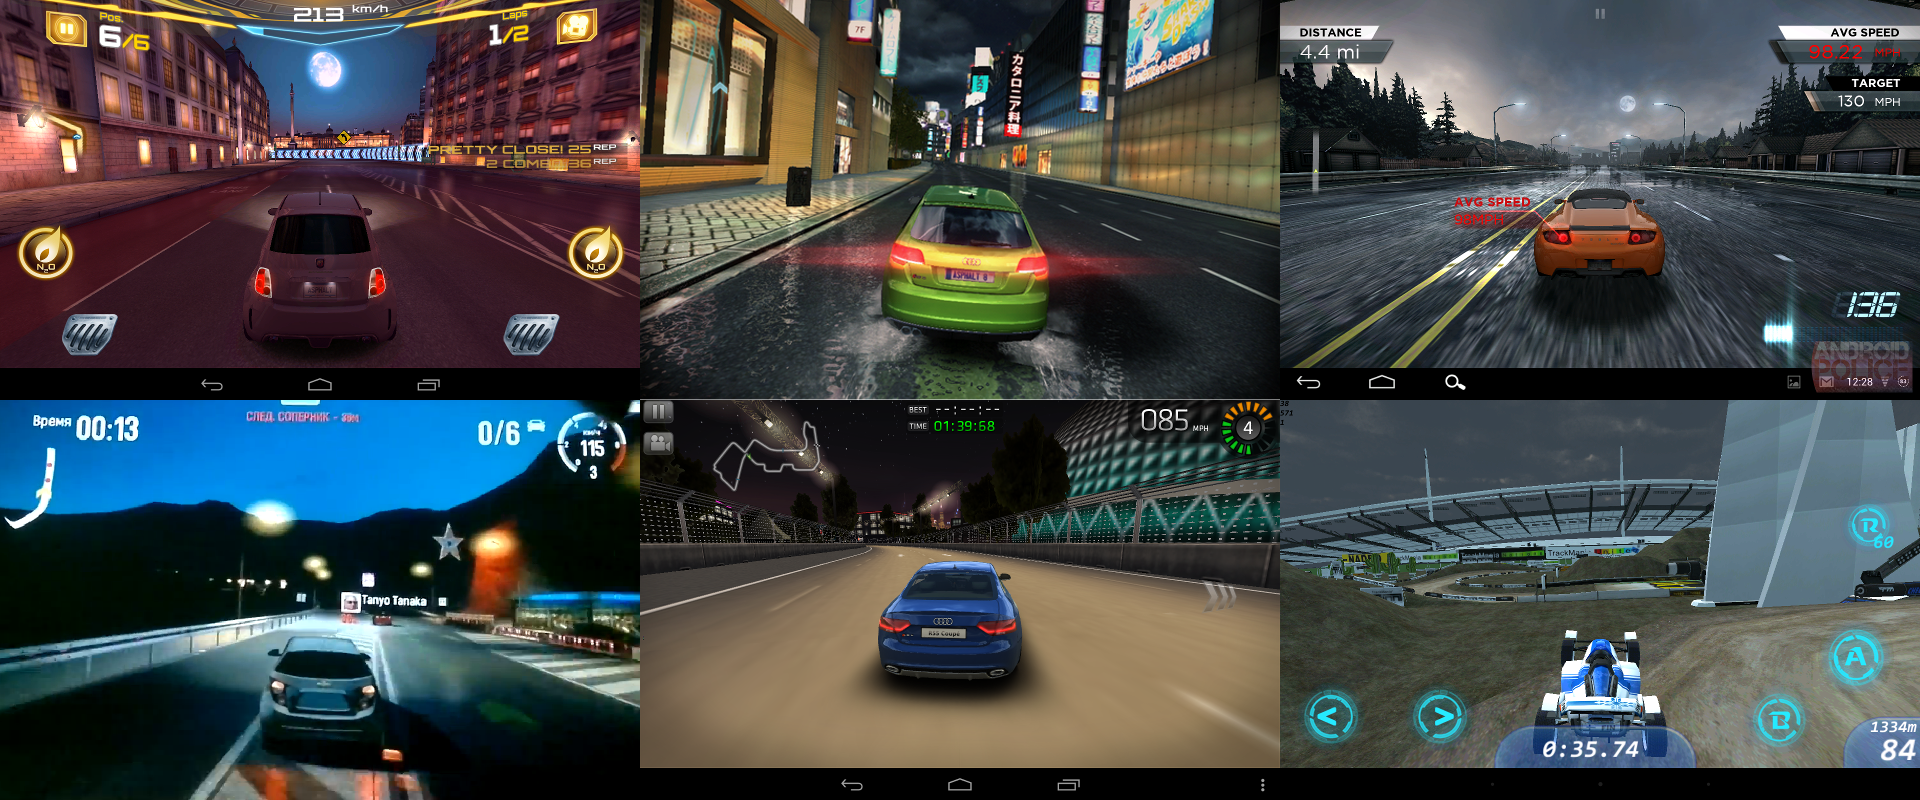
\includegraphics[width=150mm]{figures/games.png}
\caption{Ukázka závodních simulátorů s noční scénou pro platformu Android, první řada zleva: Asphalt 7, Asphalt 8, Need for Speed Most Wanted, druhá řáda zleva: GT Racing 2, Sports Car Challenge, Track Racing}
\end{figure}
\end{center}

%*****************************************************************************
\chapter{Teoretický úvod}
V této kapitole se zabývám teoretickým základem pro výpočet osvětlení povrchu těles, jejich stínování, použití míchání stínů, výpočet stínů a odlesků povrchů. Teoretický základ je nezbytný pro pochopení řešení problematiky předpočteného osvětlení.

\section{Osvětlovací model}
Osvětlovací model je funkce, která definuje odraz světla a tím i vzhled povrchů těles.\linebreak V počítačové grafice se používají lokální osvětlovací modely, které se vyznačují tím, že vypočítávají vždy pouze jeden bod na povrchu tělesa. Asi nejpoužívanější lokální osvětlovací model je Phongův. Phongův model se skládá ze tří typů osvětlení.

Výsledná intenzita osvětlení povrchu $I$ je součtem ambientní složky ($I_a$), difúzní složky ($I_d$) a spekulární složky ($I_s$).
\begin{center}
$I = I_a + I_d + I_s$\\
(Znázorněno na obrázku 3.1)
\end{center}

\begin{itemize}
\item ambientní osvětlení - nahrazuje nepřímé osvětlení konstantní hodnotou osvětlení
\item difúzní osvětlení - osvětlení nezávislé na pohledu kamery, Odpovídá ideálně matnému povrchu
\item spekulární osvětlení - osvětlení závislé na pohledu kamery, odpovídá ideálně odrazivému povrchu
\end{itemize}
\newpage

\begin{center}
\begin{figure}[h!]
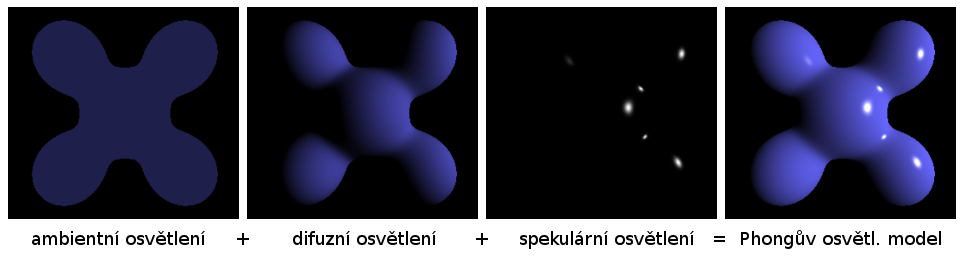
\includegraphics[width=150mm]{figures/phong.png}
\caption{Phongův osvětlovací model}
\end{figure}
\end{center}

Všesměrové osvětlení je ve Phongovo osvětlovacím modelu konstantní pro daný objekt\linebreak a říká se mu ambientní osvětlení $I_a$. Výsledná intenzita se spočte jako součin barvy ambientního světla $C_a$, koeficientem ambientního odrazu $k_a$ a barvou povrchu $C_d$, která je shodná\linebreak i pro difúzní složku.
\begin{center}
$I_a = C_a \cdot k_a \cdot C_d$
\end{center}

Difúzní složka odpovídá ideálně matnému (Lambertovskému) povrchu a závisí na úhlu $\alpha$ mezi vektory $\vec{L}$ a $\vec{N}$.
\begin{center}
\begin{figure}[h!]
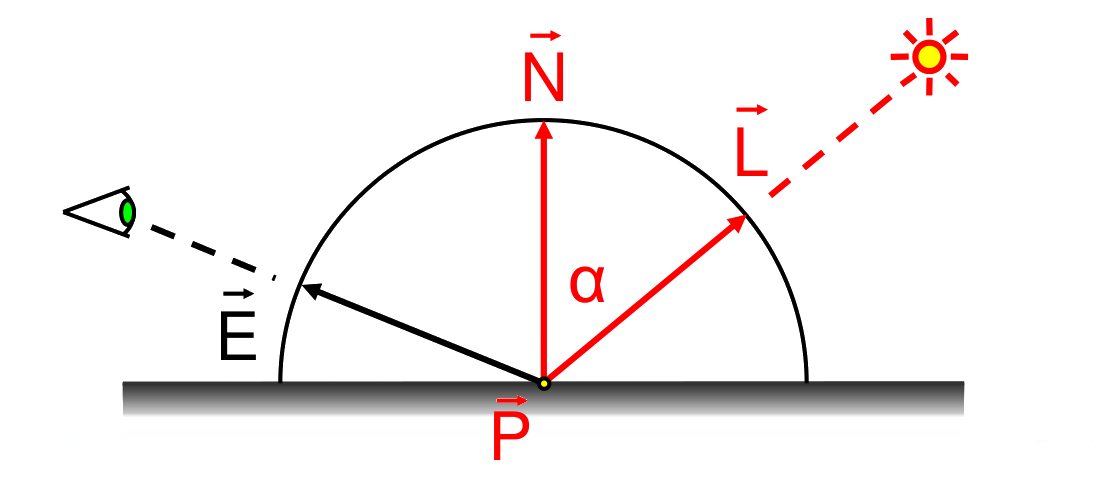
\includegraphics[width=70mm]{figures/phongD.png}
\caption{Vektory k výpočtu difúzního osvětlení, $\vec{L}$ je normalizovaný směr světla, $\vec{N}$ je normalizovaná normála povrchu, $\alpha$ je úhel, který tyto vektory svírají, $\vec{E}$ je normalizovaný směr pohledu kamery (eye vektor) a $\vec{P}$ je bod na povrchu tělesa}
\end{figure}
\end{center}
Intenzitu difúzní složky lze vyjádřit následovně.
\begin{center}
$I_d = C_l \cdot k_d \cdot C_d \cdot cos(\alpha)$
\end{center}
$C_l$ je barva světla, $k_d$ koeficient difúzního odrazu, $C_d$ barva povrchu a pro úhel $\alpha$ platí, že $cos(\alpha) = \vec{L} \cdot \vec{N}$. Po dosazení tedy získáme výsledný výraz.
\begin{center}
$I_d = C_l \cdot k_d \cdot C_d \cdot (\vec{L} \cdot \vec{N})$
\end{center}
\bigskip

Spekulární (zrcadlová) složka odpovídá ideálně odrazivému tělesu a závisí na úhlu $\beta$ mezi vektory $\vec{E}$ a $\vec{R}$. 
\begin{center}
\begin{figure}[h!]
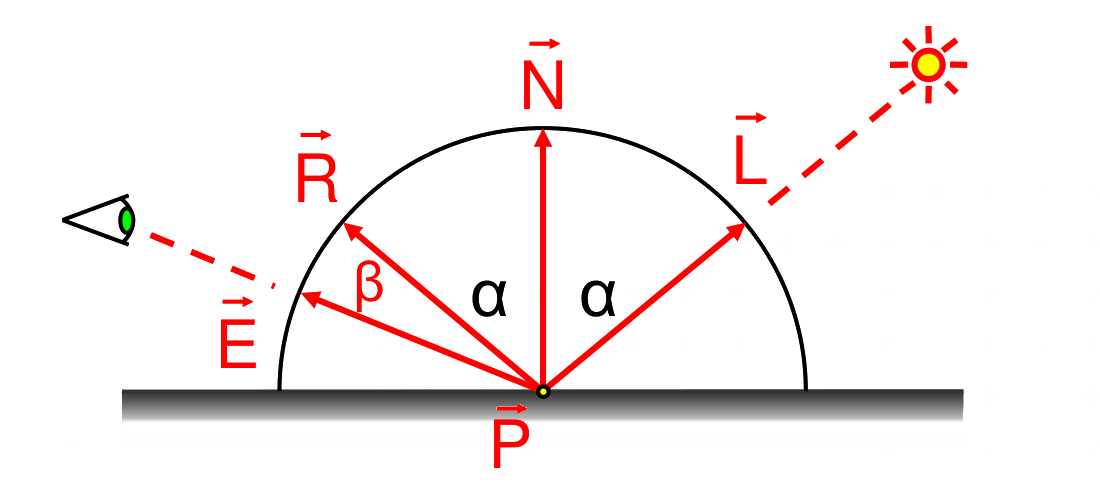
\includegraphics[width=70mm]{figures/phongS.png}
\caption{Vektory k výpočtu spekulárního osvětlení, $\vec{E}$ je normalizovaný směr pohledu kamery (eye vektor), $\vec{R}$ je normalizovaný směr odrazu světla, $\beta$ je ůhel, který tyto vektory svírají a $\vec{P}$ je bod na povrchu tělesa}
\end{figure}
\end{center}
Intenzitu spekulární složky lze vyjádřit následovně.
\begin{center}
$I_s = C_l \cdot k_s \cdot C_s \cdot cos^h(\beta)$
\end{center}
$C_l$ je barva světla, $k_s$ koeficient spekulárního odrazu, $C_s$ barva lesklého povrchu (většinou bývá bílá), $h$ je ostrost odrazu a pro úhel $\beta$ platí, že $cos(\beta) = \vec{E} \cdot \vec{R}$. Po dosazení tedy získáme výsledný výraz.
\begin{center}
$I_s = C_l \cdot k_s \cdot C_s \cdot (\vec{E} \cdot \vec{R})^h$
\end{center}

\section{Výpočet osvětlení}

Pro výpočet osvětlení konkrétního bodu na obrazovce je potřeba nejdříve spočítat příspěvky jednotlivých světel pro tento bod. Příspěvky jednotlivých světel $I_{Li}$ spočteme jako součin efektivity reflektoru pro daný vertex $E_r$, faktoru útlumu $F_a$ a součtu složek Phongova osvětlovacího modelu.
\begin{center}
$I_{Li} = E_r \cdot F_a \cdot (I_a + I_d + I_s)$
\end{center}

Efektivita reflektoru $E_r$ je parametr určující intenzitu osvětlení zdroje světla typu reflektor (znázorněno na obrázku 3.4). Příkladem takového zdroje světla je například baterka.
\newpage

\begin{center}
\begin{figure}[h!]
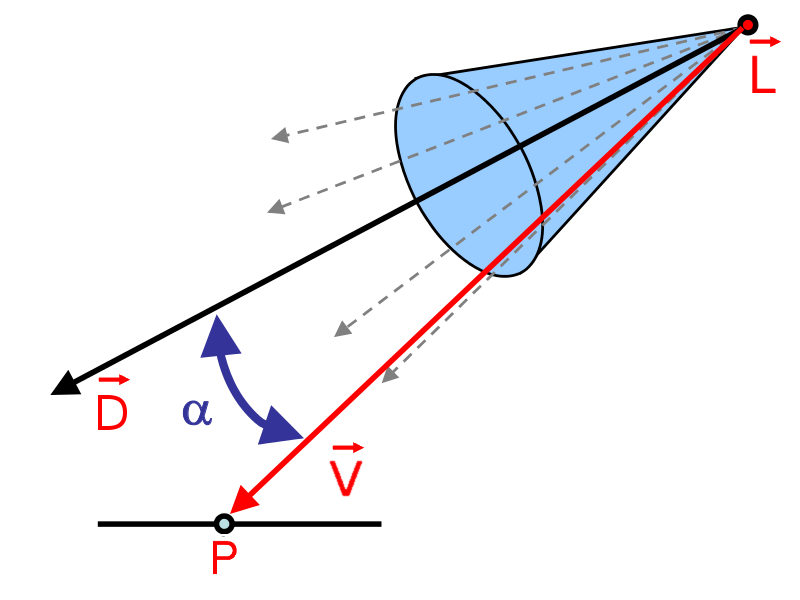
\includegraphics[width=60mm]{figures/cutoff.png}
\caption{Vektory k výpočtu efektivity reflektoru, $\vec{D}$ je normalizovaný směr světla, $\vec{V}$ je normalizovaný směr světla na kraji světelného kužele, $\alpha$ je úhel, který tyto vektory svírají, $\vec{L_p}$ je pozice zdroje světla a $\vec{P}$ je bod na povrchu tělesa}
\end{figure}
\end{center}

\noindent Hodnota efektivity reflektoru se spočte podle následujících podmínek.
\begin{itemize}
\item Pokud světlo není reflektor, poté $E_r = 1$.
\item Pokud bod leží mimo světelný kužel, tedy $(\vec{V} \cdot \vec{D}) < cos(\alpha)$, poté $E_r = 0$.
\item Pro ostatní případy $E_r = max(0, cos(\vec{V} \cdot \vec{D}))^{k_{se}}$, kde $k_{se}$ je parametr spot efektu.
\end{itemize}
\bigskip

Faktor útlumu $F_a$ řeší, jak moc má být intenzita světla utlumena s rostoucí vzdáleností $d$ od zdroje světla. Konstantní útlum určuje parametr $k_c$, lineární útlum parametr $k_l$\linebreak a kvadratický útlum parametr $k_q$.
\begin{center}
$F_a = \frac{1}{k_c + k_l \cdot d + k_q \cdot d^2}$
\end{center}
\bigskip

Výsledná barva bodu na obrazovce $I$ se spočítá jako součet barvy emisního světla $I_e$, barvy globálního ambientního světla $I_{ag}$ a sumy příspěvků jednotlivých světel $I_{Li}$.
\begin{center}
$I = I_e + I_{ag} + \sum_{}{} I_{Li}$
\end{center}
\newpage

\section{Stínování}
Pojem stínování v počítačové grafice znamená postup vybarvování trojúhelníků. Existují tři základní typy stínování.
\begin{itemize}
\item Konstantní stínování - celý polygon se vybarví jednou barvou dle normály povrchu. Používá se ve scénách, ve kterých se nacházejí pouze směrové zdroje světla.
\item Gouraudovo stínování - spočítá se osvětlení ve vrcholech a následně se interpolují hodnoty mezi vrcholy. Toto stínování je velmi rychlé. Problém nastane, pokud světlo osvětluje střed polygonu a zároveň neosvětluje nebo jen částečně osvětluje vrchol. Osvětlení je po té ve vrcholech minimální a nemůže tedy vzniknout korektně osvětlený difúzní odraz. Obdobný problém je i se spekulárním odrazem. Problémy s difúzním a spekulárním odrazem světla obvykle nenastávají současně.
\item Phongovo stínování - spočítá se osvětlení pro každý pixel polygonu na obrazovce. Dnes je to asi nejpoužívanější stínování. V OpenGL se toto stínování provádí pomocí shaderů. Vstupem do vertexového shaderu je pozice vrcholu a jeho normála. Ve vertex shaderu se provede transformace do pohledu kamery a určí se, že pozice vrcholu a normála se mají interpolovat. Po rasterizaci získáme interpolované hodnoty jako vstup ve fragment shaderu a zde provedeme výpočet podle výše uvedeného osvětlovacího modelu.
\end{itemize}

\begin{center}
\begin{figure}[h]
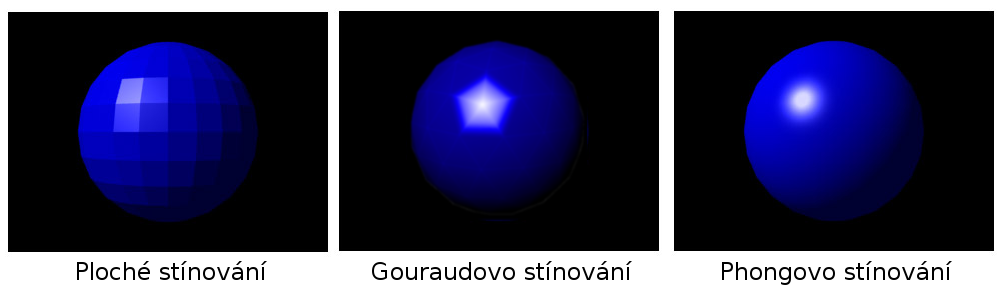
\includegraphics[width=135mm]{figures/shading.png}
\caption{Ukázka jednotlivých typů stínování}
\end{figure}
\end{center}

Interpolaci provádí OpenGL automaticky za využití barycentrických souřadnic. Barycentrické souřadnice jsou nezávislé na poloze vrcholů, znázorněno na obrázku 3.6.

\begin{center}
\begin{figure}[h]
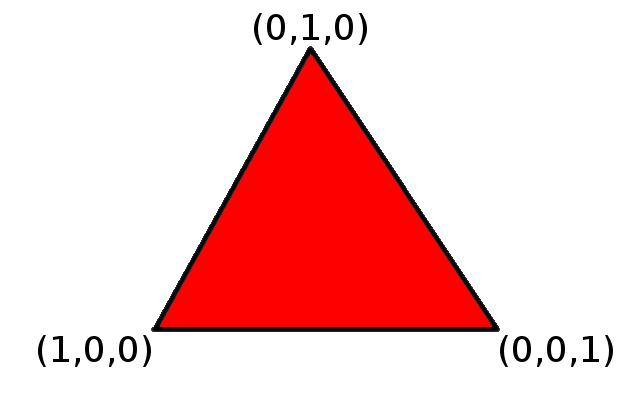
\includegraphics[width=40mm]{figures/bary.png}
\caption{Barycentrické souřadnice trojúhelníku}
\end{figure}
\end{center}

Pokud bychom chtěli získat interpolovanou hodnotu bodu $P$ pomocí barycentrických souřadnic, musíme nejdříve spočítat obsah jednotlivých trojúhelníků, abychom získali váhu hodnot v jednotlivých vrcholech.
\begin{center} 
$S_{PBC} = \frac{|\vec{PB} \times \vec{PC}|}{2}$;
$S_{APC} = \frac{|\vec{AP} \times \vec{AC}|}{2}$; 
$S_{ABP} = \frac{|\vec{AB} \times \vec{AP}|}{2}$;
$S_{ABC} = \frac{|\vec{AB} \times \vec{AC}|}{2}$
\end{center}

\begin{center}
\begin{figure}[h]
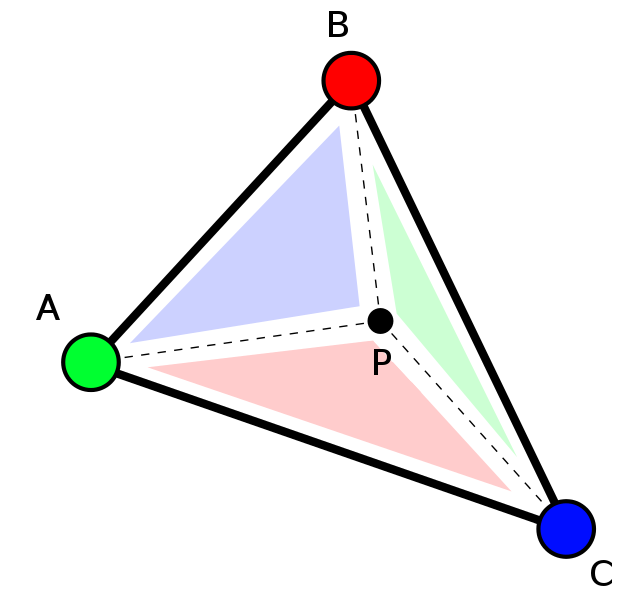
\includegraphics[width=30mm]{figures/interpolation.png}
\caption{Pomocný obrázek k výpočtu barycentrické interpolace}
\end{figure}
\end{center}

Označíme si hodnotu u bodu $A$ jako $a$, u bodu $B$ jako $b$ a u bodu $C$ jako $c$, poté získáme interpolovanou hodnotu $p$ v bodě $P$ následovně.
\begin{center}
$p = a \cdot \frac{S_{PBC}}{S_{ABC}} + b \cdot \frac{S_{APC}}{S_{ABC}} + c \cdot \frac{S_{ABP}}{S_{ABC}}$
\end{center}

\section{Míchání textur}

Míchání textur neboli blending je technika, která míchá cílový obraz (ten již vykreslený na obrazovce) a zdrojový obraz, tedy texturu namapovanou na nějaký model.

Vstupem pro blending funkci je zdrojová barva $C_s$, cílová barva $C_d$ a parametry $\alpha_s$\linebreak a $\alpha_d$, které určují pro každý kanál, jak se má hodnota míchat. Výstupem funkce je nová cílová barva $C_d$.
\begin{center}
$C_d = C_s \cdot \alpha_s + C_d \cdot \alpha_d$
\end{center}

U blendingu je důležité, zda kreslíme odzadu dopředu nebo obráceně. Při kreslení odzadu dopředu nejdříve vykreslíme neprůhlednou část scény bez blendingu a se zápisem do hloubkového bufferu. Potom vypneme zápis do hloubkového bufferu a vykreslíme geometrii s částečnou průhledností (se zapnutým blendingem). Při kreslení odpředu dozadu kreslíme objekty v opačném pořadí s tím rozdílem, že musíme u neprůhledného materiálu použít blending, abychom nepřekreslili poloprůhledné objekty v popředí.
\newpage

\begin{figure}[h]
\begin{center}$
\begin{array}{cc}
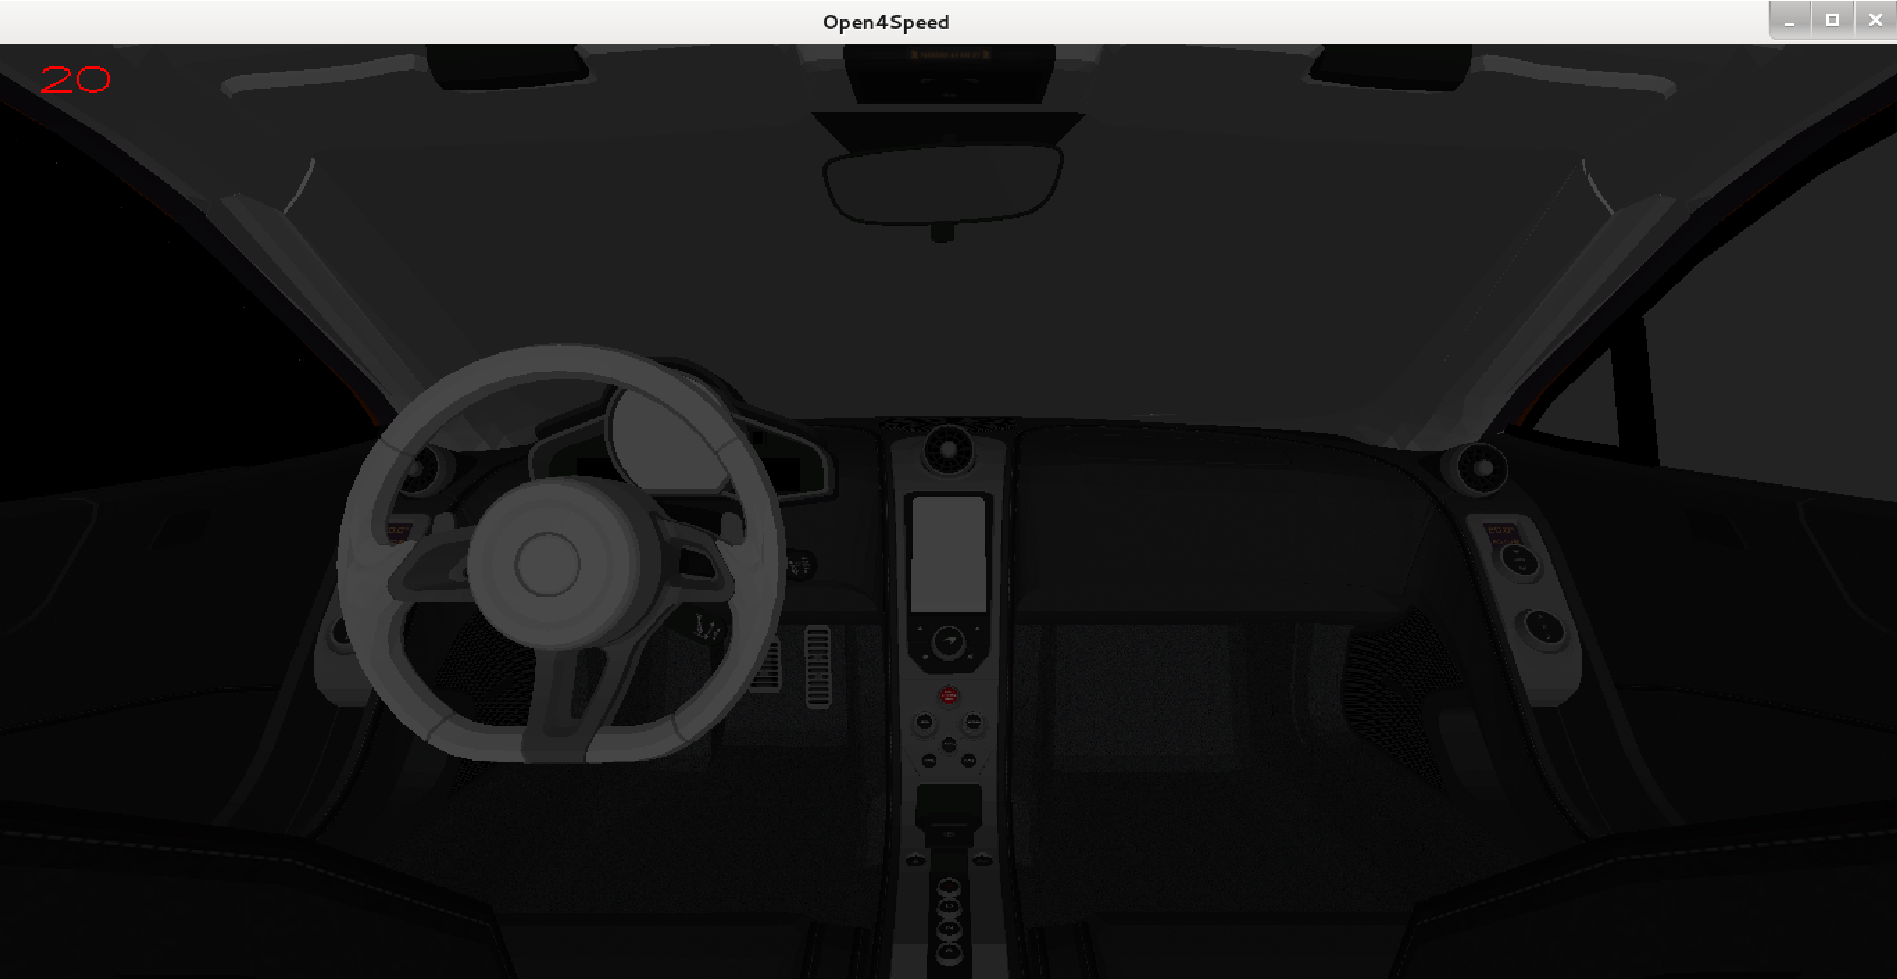
\includegraphics[width=60mm]{figures/blendoff.png} &
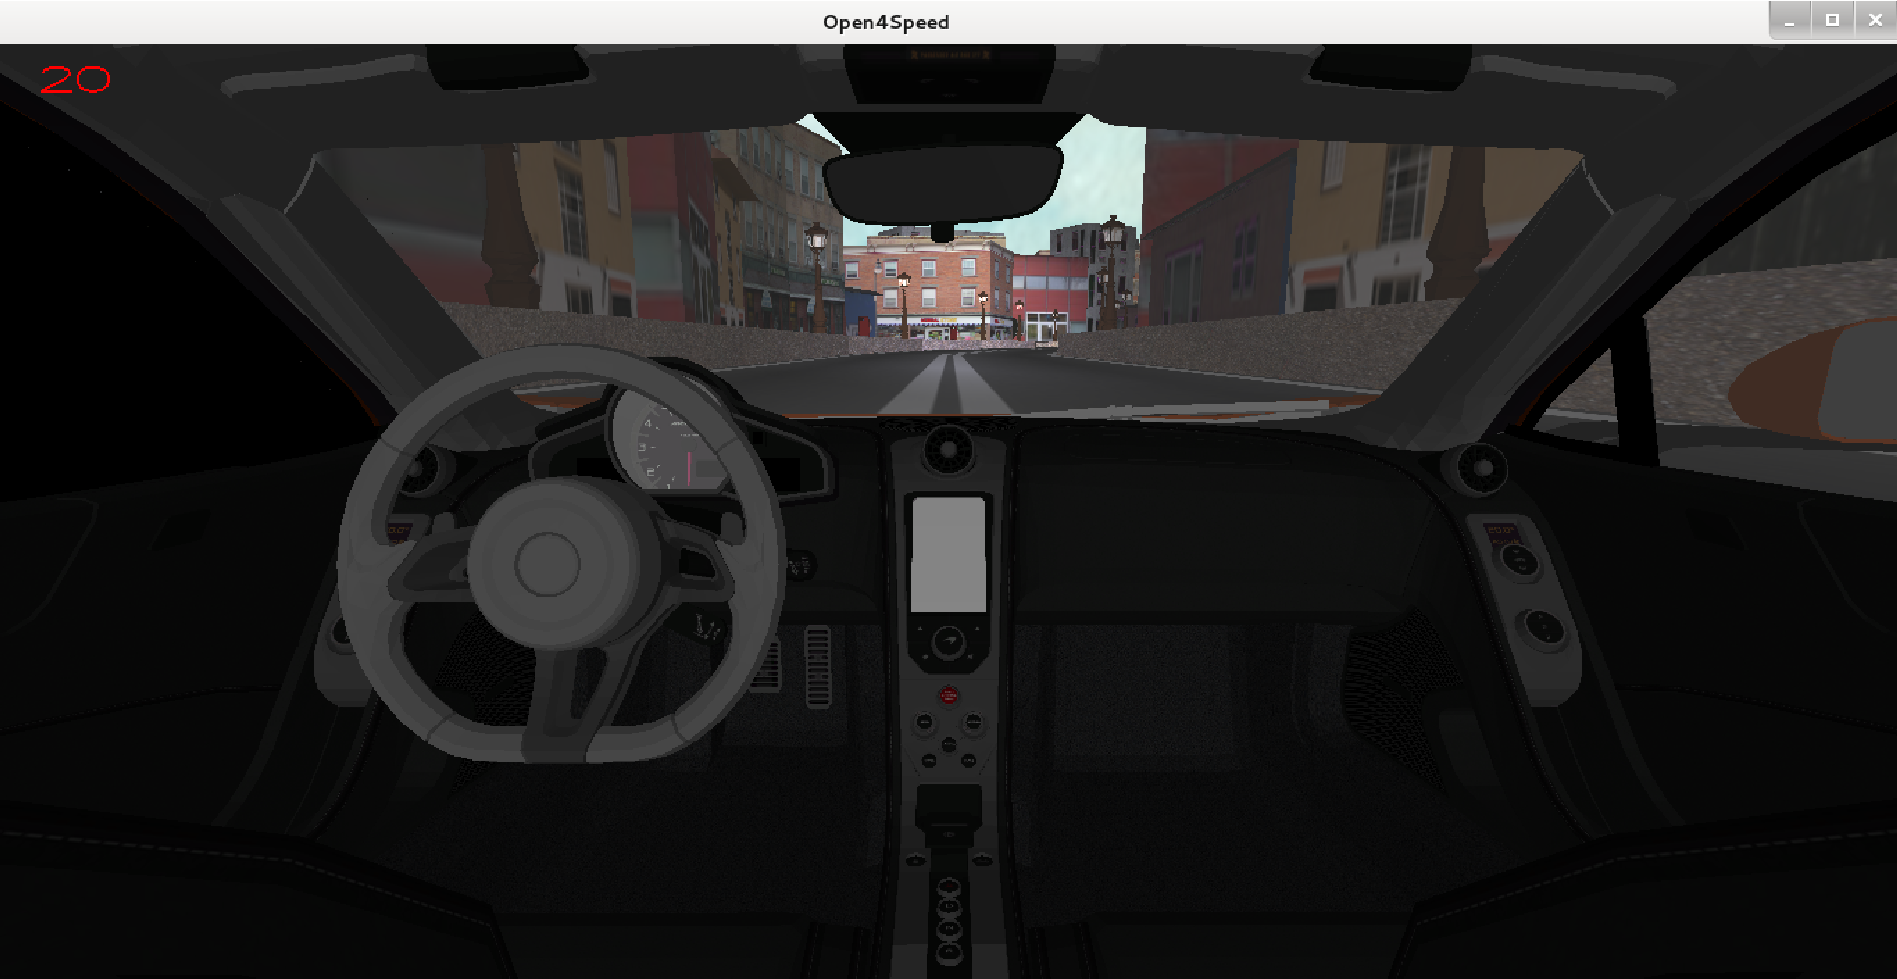
\includegraphics[width=60mm]{figures/blendon.png}
\end{array}$
\end{center}
\caption{Ukázka problému při vykreslení poloprůhledného materiálu se špatnou konfigurací}
\end{figure}

\section{Výpočet stínů}
Stíny v počítačové grafice napomáhají k vnímání souvislostí ve scéně. Pokud ve scéně stíny nepoužijeme, nebudeme například schopni poznat, zda se těleso dotýká povrchu nebo se vznáší (výjimku tvoří pohled, při kterém vzniká viditelná mezera mezi objektem a povrchem).

Abychom mohli stín spočítat, musíme znát informace o okolí aktuálně vykreslovaného primitiva. To je v OpenGL problém, protože při vykreslování primitiv nemáme standardně žádné informace o okolí. Problém se řeší pomocí tzv. stínových map. 

Stínová mapa je textura, do které se vykreslí scéna z pohledu zdroje světla. Do stínové mapy se nekreslí barevná informace, kreslí se do ní vzdálenost od zdroje světla (na obrázku 3.10 je tato vzdálenost namapovaná na odstíny šedi).

Princip stínových map je naznačen na obrázku 3.9. Při vyhodnocování bodu P se spočítá vzdálenost bodu od zdroje světla a porovná se s hodnotou uloženou ve stínové mapě.\linebreak V případě bodu P je vzdálenost vyšší než hodnota ve stínové mapě a bod je vyhodnocen jako zastíněný. V případě bodu Q je vzdálenost stejná jako ve stínové mapě (s numerickou tolerancí) a bod je tedy viditelný.

\begin{center}
\begin{figure}[h]
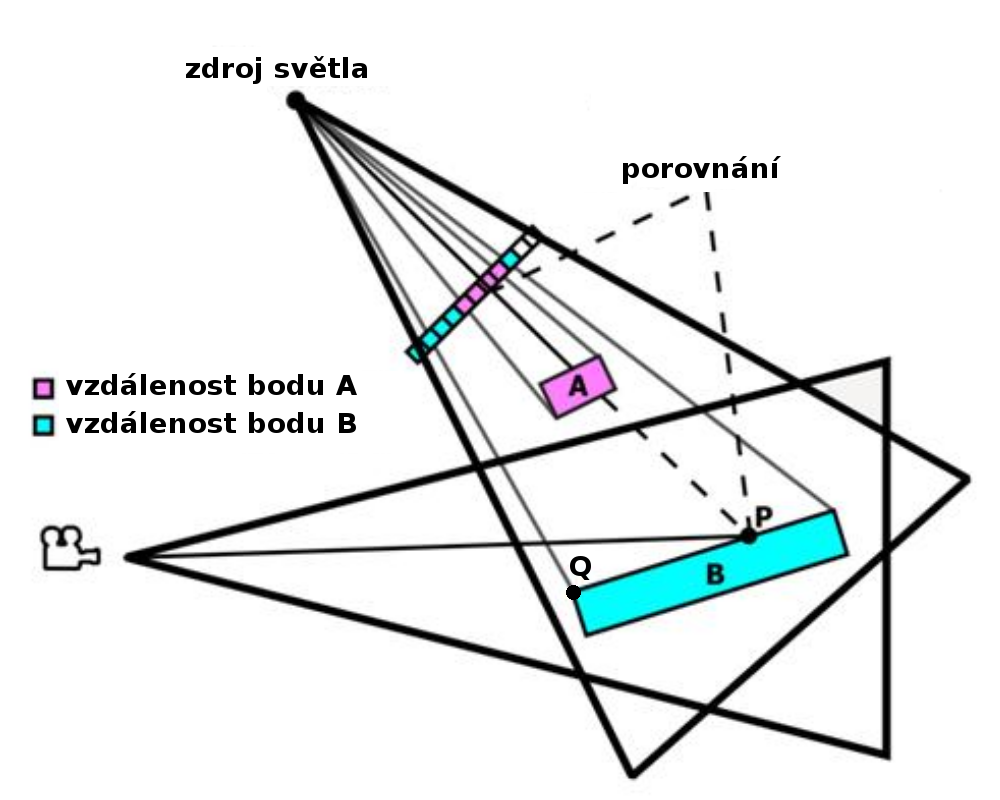
\includegraphics[width=90mm]{figures/shadowmaps.png}
\caption{Pomocný obrázek k výpočtu zastínění pomocí stínových map \cite{Ambroz12}}
\end{figure}
\end{center}

\begin{center}
\begin{figure}[h]
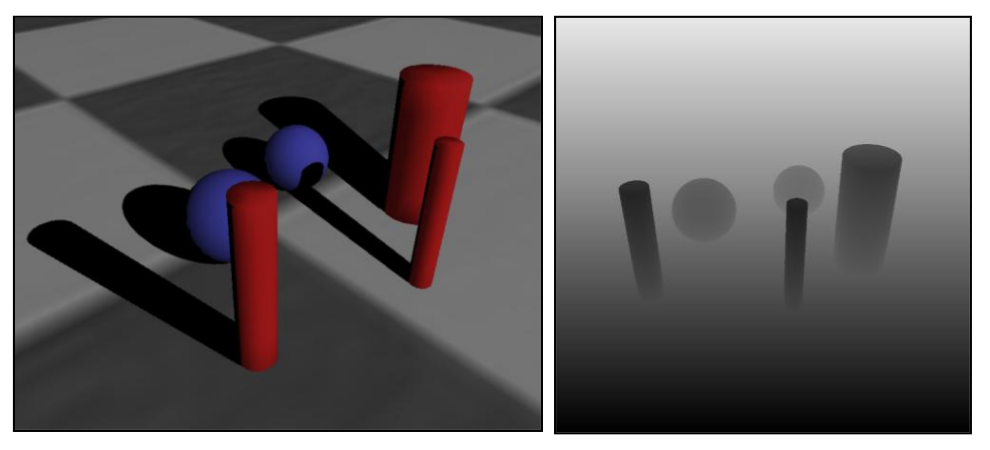
\includegraphics[width=120mm]{figures/shadowmap.png}
\caption{Ukázka scény (vlevo) a její stínové mapy (vpravo) \cite{Ambroz12}}
\end{figure}
\end{center}

Transformace ze světových souřadnic do souřadnic projekce je vyjádřen pomocí součinu modelové, pohledové a projekční matice (anglicky model, view, projection matrix, používá se zkratka MVP). Transformaci kamery si označím jako $MVP_{camera}$ a transformaci pro pohled zdroje světla jako $MVP_{light}$. Vrchol primitiva si označím jako $\vec{v}$, spočteme vektor $\vec{p}$, jehož složky $x,y$ určují pozici hodnoty ve stínové mapě a složka $z$ hodnotu texelu. Pokud bychom měli hodnotu ve stínové mapě přepisovat, zapíšeme vždy nižší hodnotu (nižší hodnota je bod bližší zdroji světla).
\begin{center}
$\vec{p} = MVP_{light} \cdot \begin{pmatrix}\vec{v}\\ 1\\\end{pmatrix}$
\end{center}

Pomocí tohoto postupu získáme stínovou mapu, kterou využijeme při vykreslování scény z pohledu kamery. Vypočteme $\vec{p}$ stejně jako při výpočtu stínové mapy a získáme vzdálenost $d$ ze stínové mapy $SM$.
\begin{center}
$d = SM[p_x, p_y]$
\end{center}

Nakonec zjistíme, jak se tyto hodnoty liší pomocí podmínky $|p_z - d| < \epsilon$, kde $\epsilon$ je malé číslo filtrující numerickou chybu. Pokud je podmínka splněna, je bod osvětlený daným zdrojem světla.
\bigskip

Výše uvedeným postupem jsou řešeny ostré stíny pro bodové zdroje světla, případně světelné reflektory. Dále je potřeba řešit měkké stíny, které vznikají z plošných zdrojů světla. Rozdíl mezi ostrými a měkkými stíny je znázorněn na obrázku 3.11.

\begin{center}
\begin{figure}[h]
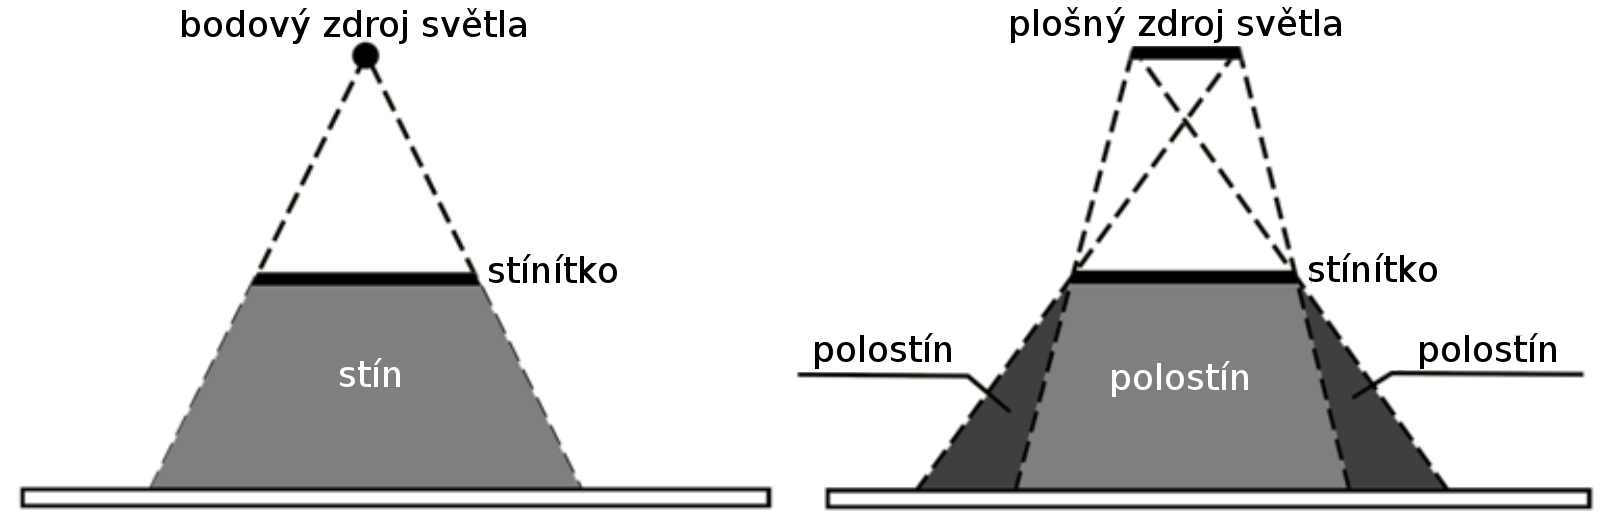
\includegraphics[width=110mm]{figures/shadows-pa.png}
\caption{Rozdíl mezi ostrými stíny (vlevo) a měkkými stíny (vpravo) \cite{Ambroz12}}
\end{figure}
\end{center}

Výpočet plošných zdrojů světel v reálném čase je stále výpočetně příliš náročný. Pro zobrazení měkkých stínů je možné použít filtrování PCF (Percentage Closer Filtering), které umožní vytvořit měkký stín pro bodový zdroj světla.

Filtrování PCF je snadno implementovatelné, vrací dobré výsledky, ale může být náročnější na výpočetní výkon. Princip filtrování PCF je, že při výpočtu zastínění se ze stínové mapy vyhodnocují i okolní body a tím vzniká přechod mezi zastíněnými a nezastíněnými pixely na obrazovce.

\begin{center}
\begin{figure}[h]
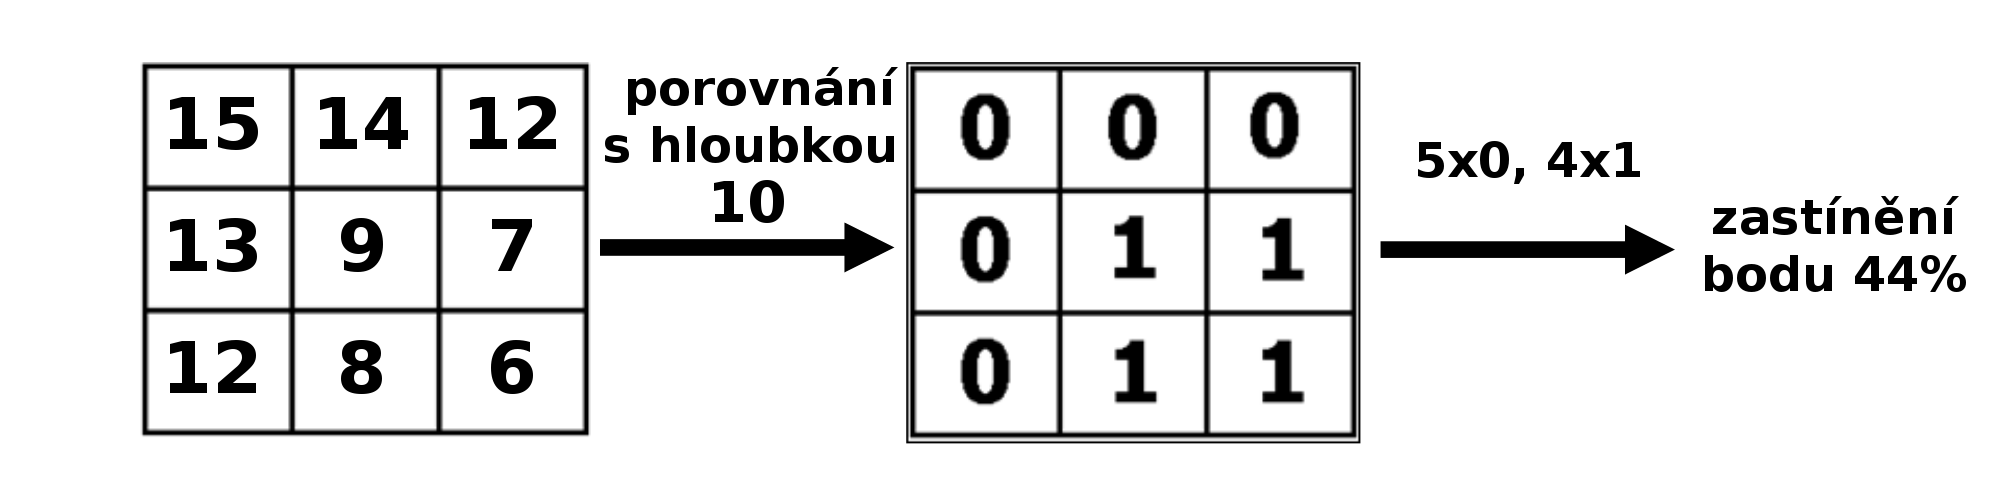
\includegraphics[width=85mm]{figures/pcf.png}
\caption{Ukázka vyhodnocení zastínění pomocí PCF 3x3. Vlevo jsou data ze stínové mapy, uprostřed vyhodnocení zastínění jednotlivých bodů (0 je viditelný bod, 1 je zastíněný bod) a vpravo výsledné zastínění}
\end{figure}
\end{center}

\begin{center}
\begin{figure}[h]
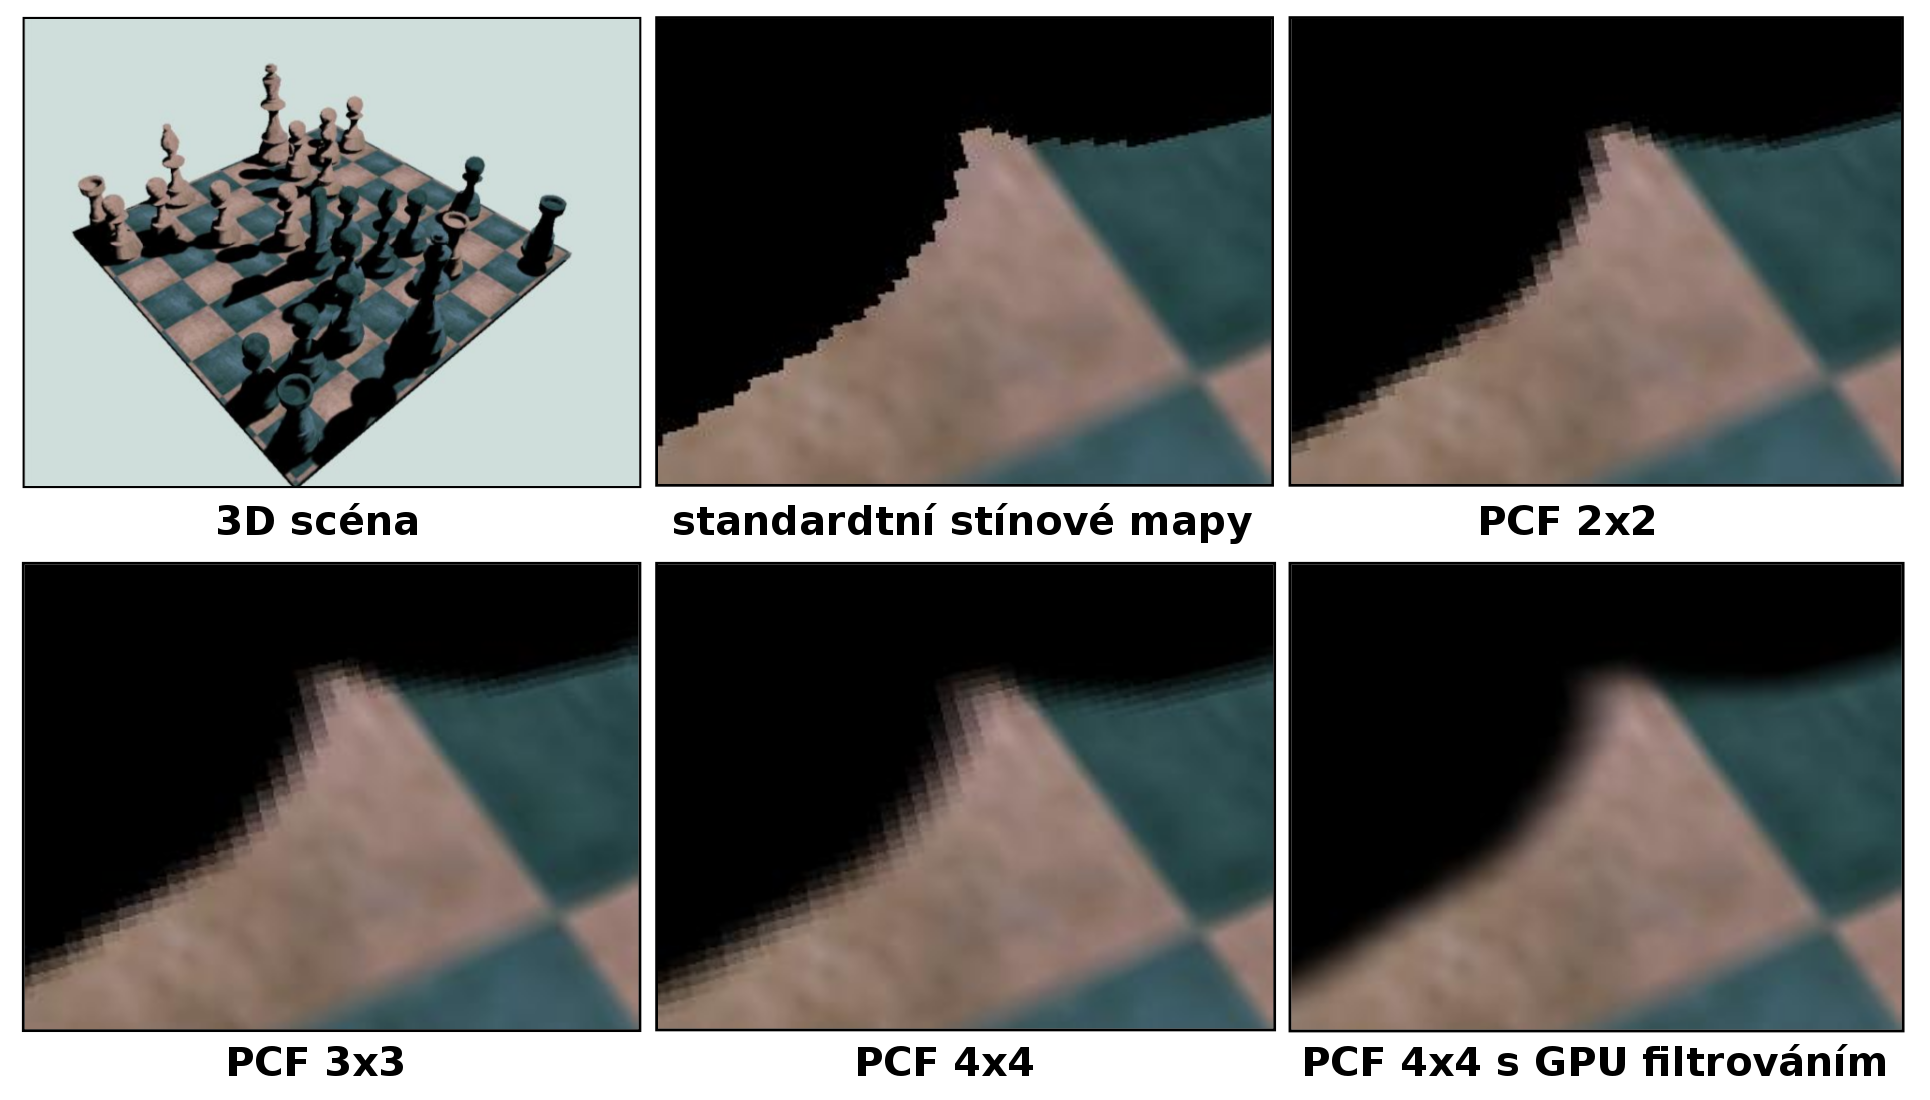
\includegraphics[width=100mm]{figures/pcf-example.png}
\caption{Ukázka výsledků filtrování PCF \cite{Ambroz12}}
\end{figure}
\end{center}
\newpage


\section{Odlesky povrchů}
Odlesky dodávají scéně lepší vzhled, dodávají dojem buď kovového nebo mokrého povrchu. V rasterizačním řetězci jsou odlesky problematické, protože grafická karta vždy zpracovává pouze aktuální geometrii a nemá informace o okolí.

Standardně se odlesk realizuje dalším průchodem, ve kterém se vykreslí okolí do textury\linebreak a tato textura se poté aplikuje na model s odleskem. U menších objektů, jako je například auto, se vykreslí okolí pomocí cube mapování do FBO. Výsledná textura se následně namapuje na objekt a tím se získá dojem lesklého povrchu.

V případě rovných povrchů je nutné použít jiný přístup, scéna se vykreslí do textury\linebreak z pohledu pod povrchem, který je na obrázku 3.14 označen jako $P'$. Pohled snímá objekty jakoby z povrchu a při vykreslování na obrazovku se spočítá pozice daného pixelu povrchu ve vykreslené textuře a z té se aplikuje barva pixelu.

\begin{figure}[h!]
\begin{center}
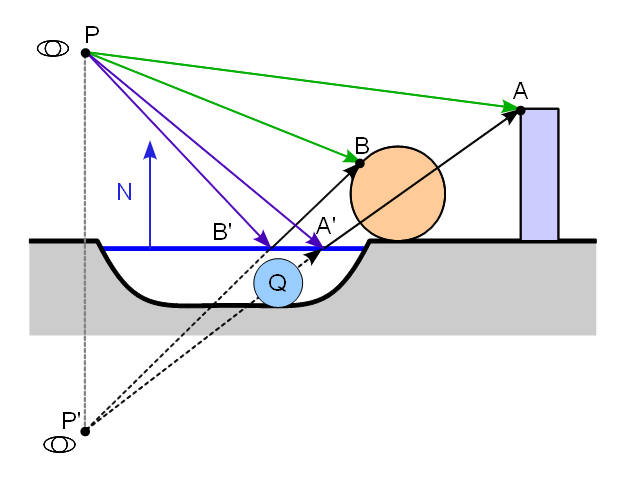
\includegraphics[width=80mm]{figures/reflection-diagram.png}
\caption{Diagram odrazu vodní hladiny \cite{Kaplinski11}}
\end{center}
\end{figure}

Pohled $P$ je MVP matice, pro získání pohledu $P'$ potřebujeme vypočítat reflexní matici $R$, která převrátí pohled podle normály povrchu $\vec{N}$ a parametru $d$ spočítaného z rovnice roviny.
              
\begin{center}
$d = -(xN_x + yN_y + zN_z)$
\end{center}
\begin{center}
$R = \begin{pmatrix}
1 -2 \cdot {\vec{N}_x}^2 & -2 \cdot N_x \cdot N_y & -2 \cdot N_x \cdot N_z & -2 \cdot N_x \cdot d\\
-2 \cdot N_y \cdot N_x & 1 -2 \cdot {N_y}^2 & -2 \cdot N_y \cdot N_z & -2 \cdot N_y \cdot d\\
-2 \cdot N_z \cdot N_x & -2 \cdot N_z \cdot N_y & 1 -2 \cdot {N_z}^2 & -2 \cdot N_z \cdot d\\
0 & 0 & 0 & 1
\end{pmatrix}$
\end{center}

Vynásobením matice $R$ s maticí $P$ získáme reflekční matici, která otáčí obraz o $180^{\circ}$, abychom získali korektní pohled, musíme provést ještě rotaci kolem osy Z.
\begin{center}
$P' = R \cdot P \cdot \begin{pmatrix}
-1 & 0 & 0 & 0\\
0 & -1 & 0 & 0\\
0 & 0 & 1 & 0\\
0 & 0 & 0 & 1
\end{pmatrix}$
\end{center}

Při vykreslování reflexního pohledu je nutné provést ořez scény pod povrchem a nevykreslovat odvrácené trojúhelníky. Pro finální vykreslování si označím reflexní mapu jako $RM$ a vykreslovaný vrchol jako $\vec{v}$. Barva odlesku $I_r$ se spočítá dle níže uvedeného vzorce.
\begin{center}
$\vec{p} = P' \cdot \begin{pmatrix}
\vec{v}\\
1
\end{pmatrix}$
\end{center}
\begin{center}
$I_r = RM[p_x, p_y]$
\end{center}

\chapter{Předpočtené osvětlení}
Předpočtené osvětlení je z hlediska vykreslování poměrně jednoduchá technika. Na 3D model se aplikuje další textura či textury, které mají vlastní texturovací souřadnice a nesou v sobě informaci o osvětlení jednotlivých trojúhelníků. Těmto texturám se říká mapy osvětlení\cite{Advanced05} a dalo by se říct, že se jedná o techniku, která rozšiřuje techniku předpočtených stínů.

Z hlediska generování těchto textur je tato technika náročnější než výsledné vykreslování, skládá se z několika kroků. V prvním kroku je třeba vytvořit texturovací souřadnice pro jednotlivé trojúhelníky.

\section{Mapy osvětlení}
\begin{center}
\begin{figure}[h!]
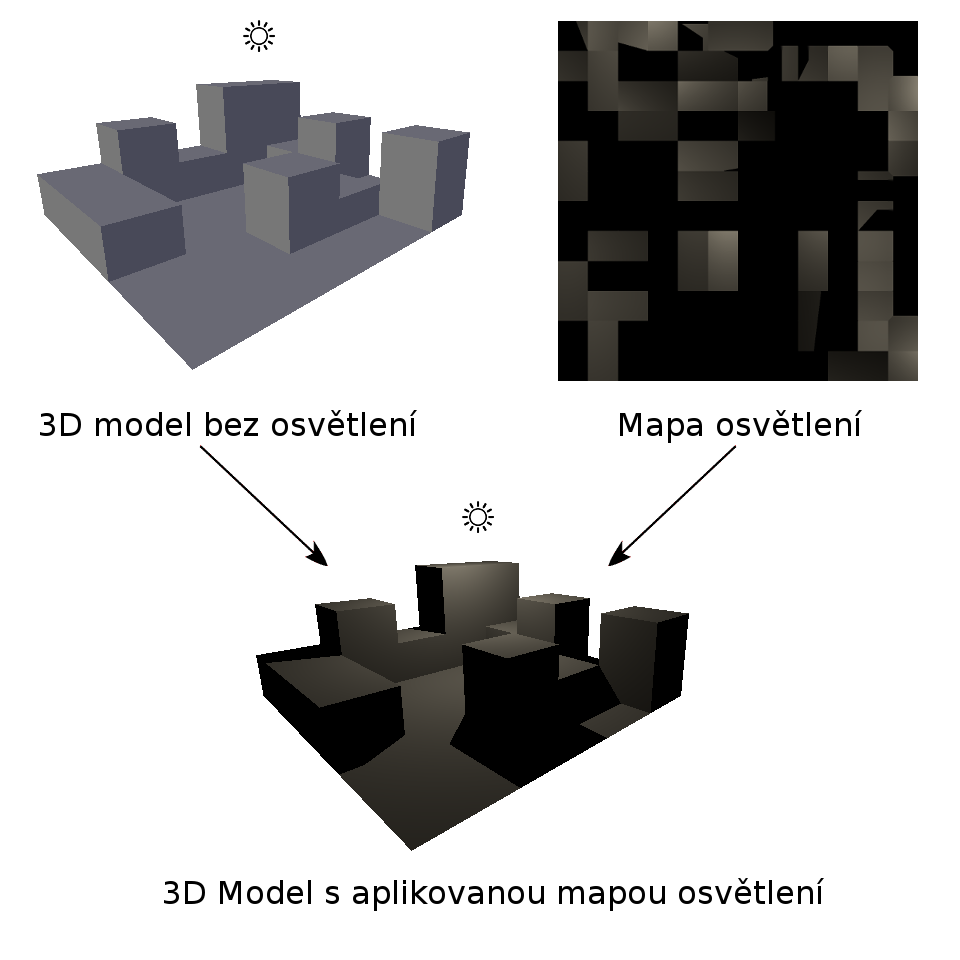
\includegraphics[width=80mm]{figures/lmapply.png}
\caption{Ukázka mapy osvětlení na jednoduchém 3D modelu}
\end{figure}
\end{center}
\newpage

Aby bylo možné mapy osvětlení dynamicky aktualizovat, je potřeba mít do map rychlý zapisovací přístup. Pro aktualizaci musíme mít předpočítanou tzv. záplatu. Záplatou se rozumí menší textura, která se přidá do současné osvětlovací mapy. Přidáním záplaty lze tedy přidat do scény další světlo, které máme předpočítané. Záplata jde z mapy osvětlení opět odebrat (provede se odečet stejné záplaty).

Protože uchovávání záplat v paměti by bylo příliš paměťově náročné, jsou komprimovány ve vektorové podobě přímo na GPU. Vektorová podoba záplaty je množina trojúhelníků,\linebreak u kterých jsou vrcholy definovány 2D polohou v mapě osvětlení a intenzitou světla. Intenzita světla se při aplikování násobí barvou, která je pro celou záplatu konstantní.

\begin{center}
\begin{figure}[h!]
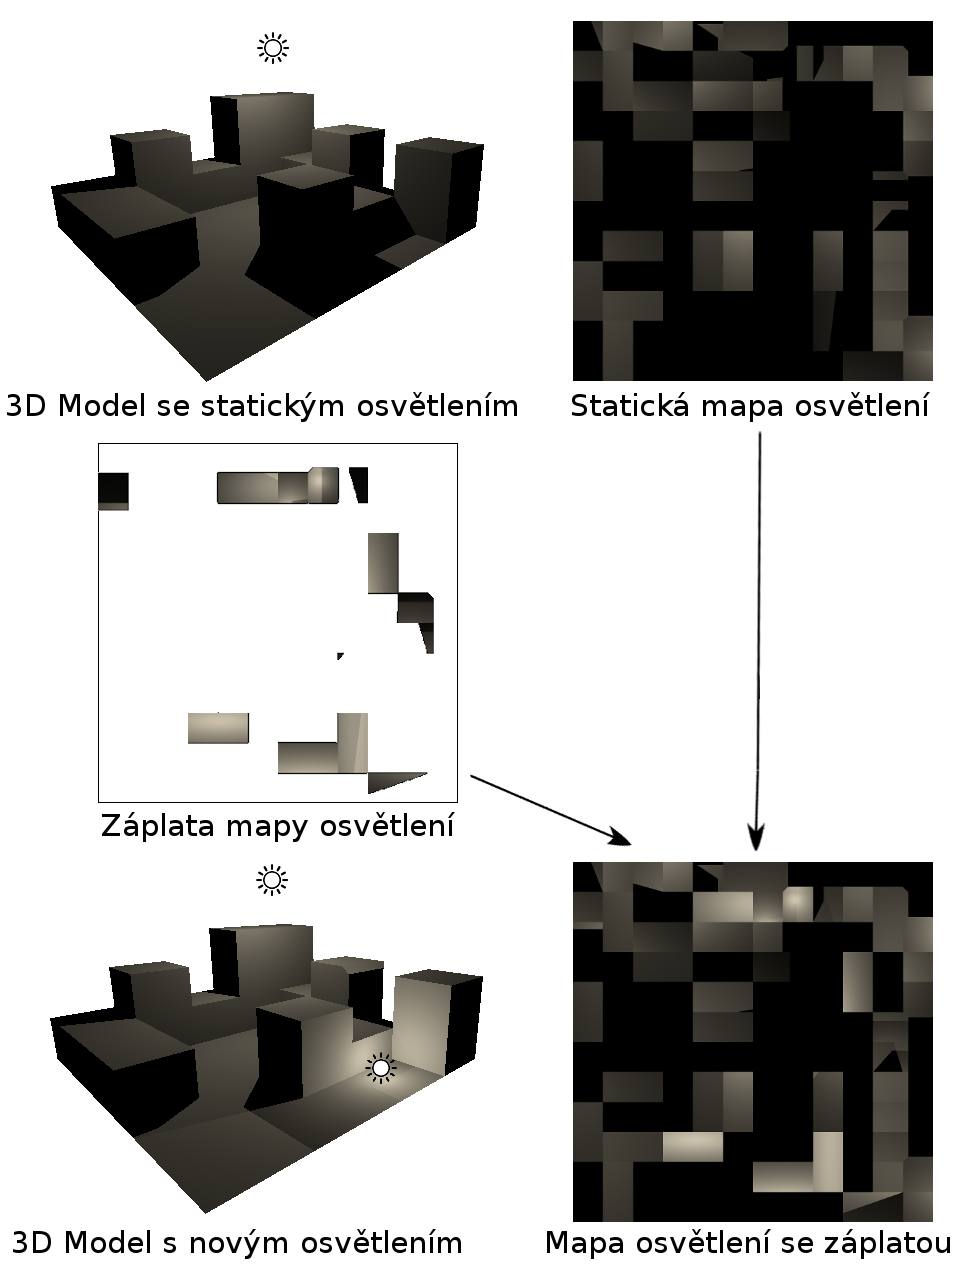
\includegraphics[width=90mm]{figures/lmupdate.png}
\caption{Ukázka aktualizace map osvětlení na jednoduchém 3D modelu, žlutou barvou je znázorněna část záplaty, která nenese informaci o změně osvětlení}
\end{figure}
\end{center}
\newpage

\section{Vytvoření texturovacích souřadnic}
Pro mapy osvětlení není vhodné použít standardní texturovací souřadnice. V osvětlovacích mapách je potřeba zajistit, aby každý texel mapy odpovídal právě jednomu bodu\linebreak v prostoru. Pokud by tomu tak nebylo, stalo by se, že při osvětlení jednoho bodu se rozzáří\linebreak i jiný bod než ten osvětlený. Problém vytváření texturovacích souřadnic se nazývá problém rozvinutí modelu\cite{Creating13} (anglicky unwrap).

Obsah povrchu 3D modelu v ideálním případě odpovídá obsahu ploch map osvětlení. Abychom se tomuto případu přiblížili, musíme plochu map co nejvíce využít. Maximálním využitím 2D plochy se zabývá problém batohu, který patří do kategorie problémů NP-hard (obtížný nedeterministický problém řešitelný v polynomiálním čase).

Běžně se problém batohu zabývá pouze osově zarovnanými obálkovými tělesy (AABB). V této práci tento problém rozšiřuji o práci s trojúhelníky. Řešení spočívá ve spojování trojúhelníků do tvaru obdélníku, aby bylo možné problém řešit jako běžný problém batohu.

\begin{center}
\begin{figure}[h]
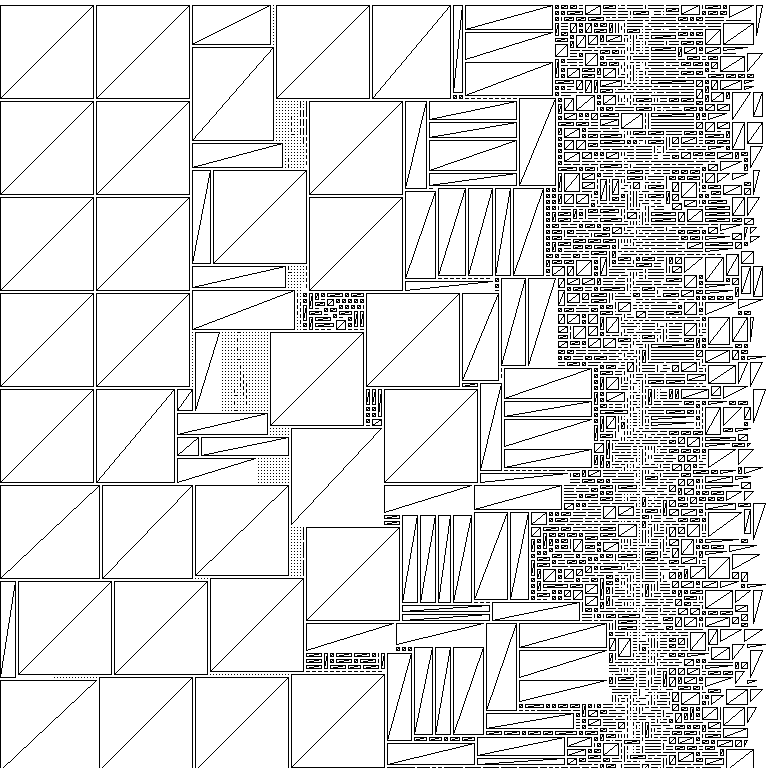
\includegraphics[width=60mm]{figures/lmcoords.png}
\caption{Výsledek řešení problému batohu se spárovanými trojúhelníky}
\end{figure}
\end{center}

Problém batohu lze řešit pomocí ILP (Integer Linear programming). Problém lze přeformulovat pomocí kolizí dvou AABB. Pokud si všechny levé horní body AABB označím souřadnicemi $[minx, miny]$ a pravé dolní souřadnicemi $[maxx, maxy]$, platí poté následující výraz, pomocí kterého lze sestrojit ILP řešení (toto řešení neuvažuje otáčení AABB).

$\forall_{i,j}, i \neq j: (minx_i < maxx_j) \cap (miny_i < maxy_j) \cap (maxx_i > minx_j) \cap (maxy_i > miny_j)$
\bigskip

Abychom mohli problém řešit tímto způsobem, musíme mít nejdříve AABB místo trojúhelníků. Vytvoření AABB se zde provádí pomocí párování trojúhelníků. 

V prvním kroku se spočítá Eulerovská délka jednotlivých hran, nejdelší hranu označíme jako $c$ (to je přepona). Pokud chceme vytvořit plně využité AABB musíme mít všechny trojúhelníky pravoúhlé, z toho důvodu původní $c$ zahodíme a vytvoříme pravoúhlý trojúhelník o délce stran $a, b$. Pro novou přeponu platí $c' = \sqrt{a^2 + b^2}$.

\begin{center}
\begin{figure}[h]
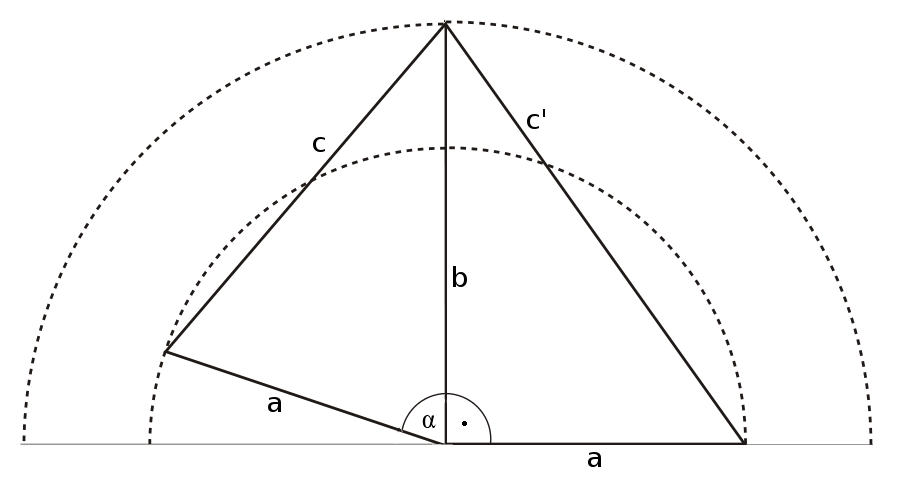
\includegraphics[width=80mm]{figures/triangle.png}
\caption{Změna délky přepony trojúhelníka pro vytvoření páru dvou trojúhelníků, vlevo původní nepravoúhlý trojúhelník, vpravo trojúhelník s novou délkou přepony}
\end{figure}
\end{center}

V dalším kroku hledáme párové trojúhelníky se stejnými délky stran $a, b$ (s určitou tolerancí), párové se spojí přeponou k sobě. Pro nepárové trojúhelníky vytvoříme AABB\linebreak o velikosti $a, b$ a tím máme vyřešený problém párování trojúhelníků.

\paragraph{Oprava chyby sousedících trojúhelníků}\mbox{}\\

Při použití výše uvedeného postupu vzniká problém při vykreslování, protože není\linebreak u texelů kolem přepon jednoznačné, ke kterému trojúhelníku texel patří, a proto vznikají ve výsledné scéně artefakty. Stává se to, protože sousedící trojúhelníky v mapě osvětlení spolu nesousedí ve scéně.

\begin{center}
\begin{figure}[h]
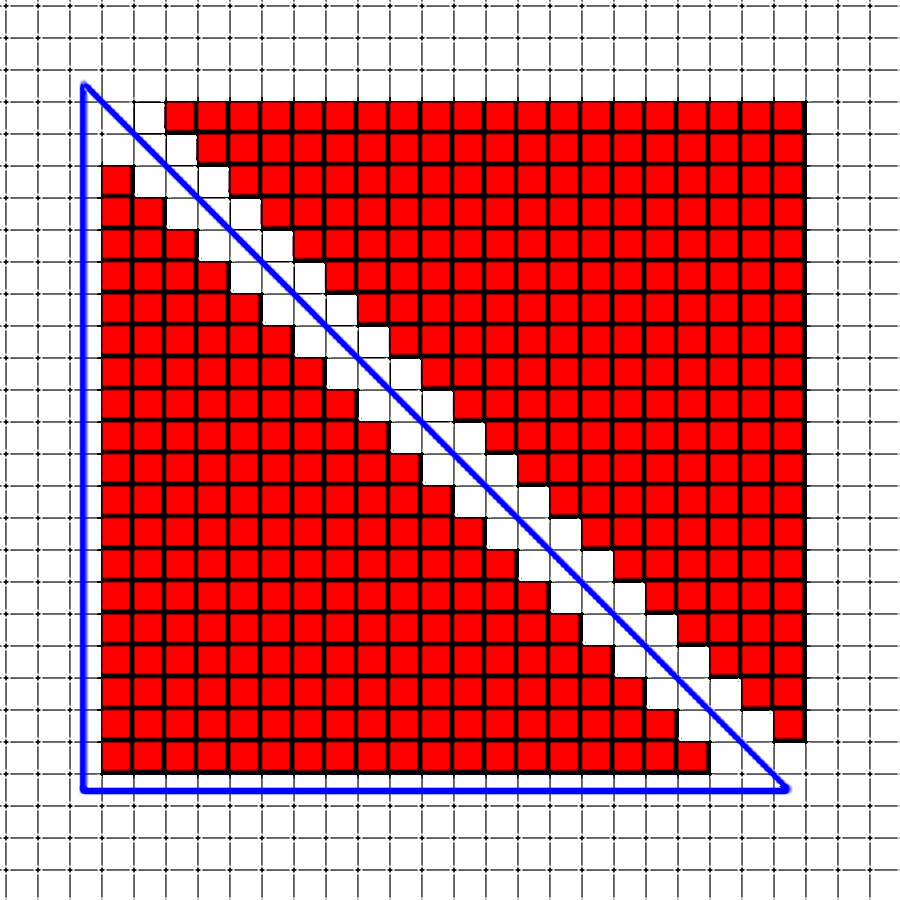
\includegraphics[width=60mm]{figures/lmfix.png}
\caption{Problém kolizních texelů dvou trojúhelníků}
\end{figure}
\end{center}

Provádí se zde posun texturovacích souřadnic směrem dovnitř trojúhelníku, aby k tomuto problému nedocházelo. Posouvají se i osově zarovnané hrany, protože při použití lineárního filtrování textur by docházelo k obdobným artefaktům jako v případě přepon.

\section{Generování map osvětlení}
Používají se dvě základní metody generování map osvětlení, pomocí vrhání či sledování paprsku a pomocí rasterizace. V metodě vrhání paprsku se vrhají primární paprsky pro každý pixel na obrazovce (tím se zjistí cílový bod ve scéně, který bude zobrazen na dané pozici). Po té se vrhnou z každého bodu sekundární paprsky do všech zdrojů světel a zjistí se, jak je bod osvětlen. Viz. obrázek 4.6.

\begin{center}
\begin{figure}[h]
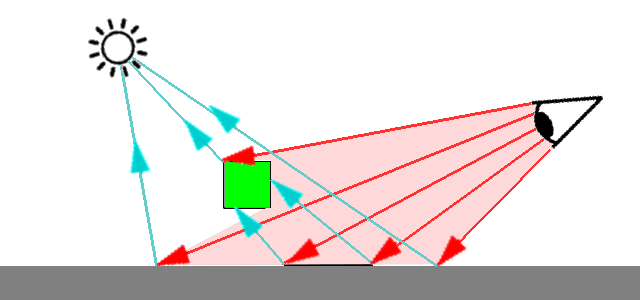
\includegraphics[width=50mm]{figures/raycasting.png}
\caption{Metoda vrhání paprsků, červeně jsou zobrazeny primární paprsky, modře stínové paprsky}
\end{figure}
\end{center}

Rasterizační metoda vykresluje narozdíl od metody vrhání paprsků scénu kompletně, jednotlivé fragmenty se kreslí přes sebe a prioritu má vždy ten fragment, který je blíže\linebreak ke kameře. Místo stínových paprsků se zde používají stínové mapy (viz. kapitola 3.5).

\begin{center}
\begin{figure}[h]
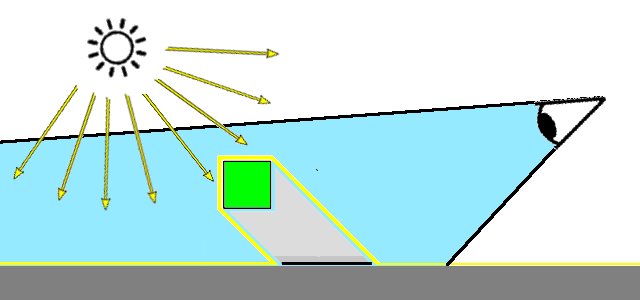
\includegraphics[width=50mm]{figures/shadowmapping.png}
\caption{Rasterizační metoda}
\end{figure}
\end{center}

U rasterizační metody lze využít k generování map osvětlení stínových map stejným způsobem, jako se používají k výpočtu zastínění v reálném čase. Rozdíl je pouze v transformování vrcholů a ve výpočtu barvy (nechceme vykreslovat texturu do světelných map, vedlo by to ke ztrátě kvality textur).

Nejdříve si vložíme ke každému vrcholu do VBO jeho souřadnice v osvětlovací mapě. Transformujeme vrchol do souřadnic mapy osvětlení. To se provede přiřazením souřadnic $u, v$ jako pozici ve FBO (s pozicí vrcholu se počítá pouze při výpočtu osvětlení).

Výslednou barvu texelu $C_t$ vypočteme z difúzního osvětlení pomocí níže uvedeného vzorce, kde $E_r$ je efektivita reflektoru, $F_a$ faktor útlumu, $C_l$ barva světla, $k_d$ koeficient difúzního odrazu, $\vec{L}$ je normalizovaný směr světla a $\vec{N}$ je normalizovaná normála povrchu. Více informací k výpočtu v kapitole 3.1.
\begin{center}
$C_t = E_r \cdot F_a \cdot C_l \cdot k_d \cdot (\vec{L} \cdot \vec{N})$
\end{center}

Pokud bychom chtěli použit i bodové zdroje světla, musíme mít stínovou mapu pro všechny možné směry světelných paprsků. K tomu lze využít tzv. mapování na krychli. Mapování na krychli je mapování scény, při kterém se na každou stěnu krychle vykreslí pohled v jednom směru s perspektivním úhlem $90^{\circ}$. V případě použití stínových map při mapování na krychli, se pro každou stranu provádí výpočet, jakoby se jednalo o samostatné světlo (efektivita reflektoru $E_r = 1$).

\begin{center}
\begin{figure}[h]
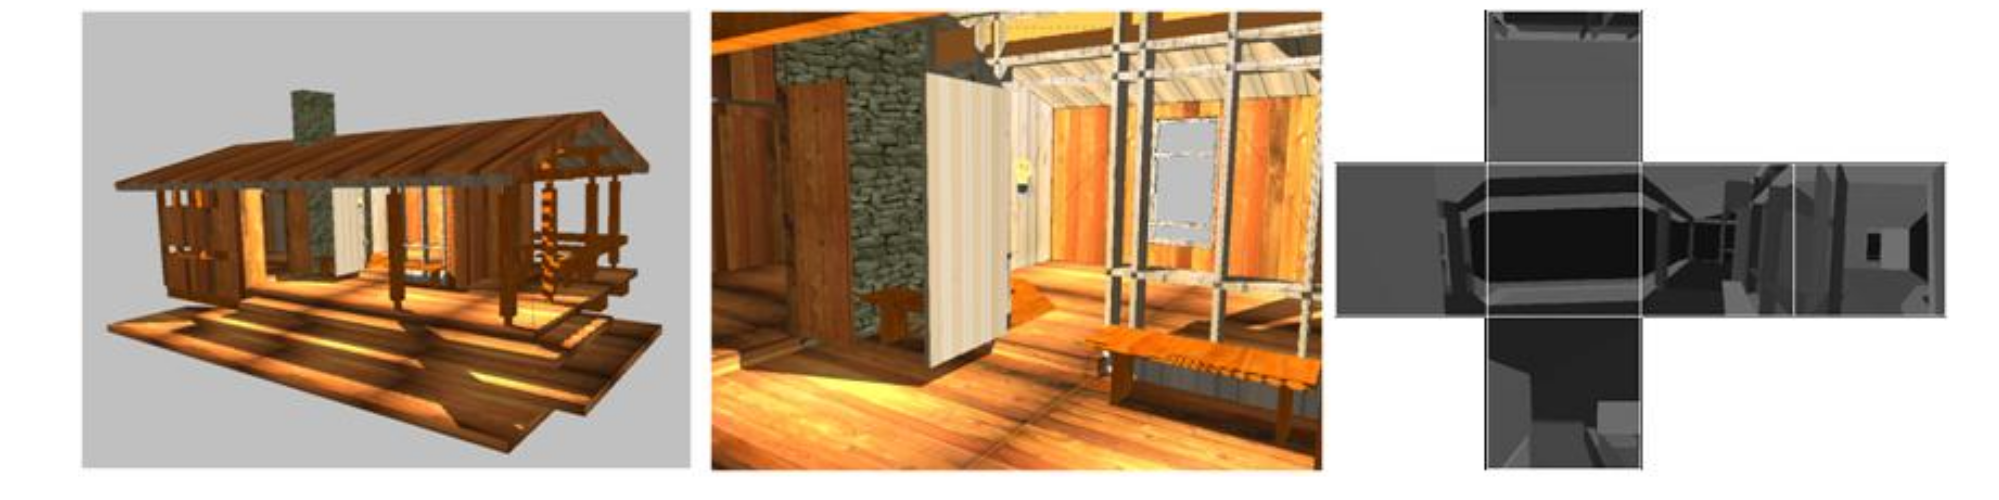
\includegraphics[width=130mm]{figures/cubemap.png}
\caption{Využití stínových map při mapování na krychli u bodových světel, vlevo dva náhledy scény, vpravo stínová mapa \cite{Ambroz12}}
\end{figure}
\end{center}

\section{Spekulární složka osvětlovacího modelu}
Spekulární složka osvětlovacího modelu je závislá na pohledu kamery a nelze jí tedy předpočítat a také nelze počítat v reálném čase spekulární složky pro desítky světel. Tento problém se dá řešit vypnutím vzdálených světel. Světla se seřadí podle vzdálenosti\linebreak od kamery a provede se započítání $n$ nejbližších (konstantu $n$ je vhodné mít co nejnižší, protože spekulární složka je poměrně náročná na výpočet). 

Nutno podotknout, že tento přístup neřeší viditelnost světla. Stejný přístup lze použít\linebreak i pro difúzní osvětlení, ale předpočtené osvětlení je efektivnější.

%*****************************************************************************
\chapter{Implementace}
Realizace projektu byla provedena ve třech fázích. Nejdříve byla vytvořena verze pro PC bez předpočteného osvětlení, dále bylo provedeno portování projektu na Android\linebreak a v poslední fázi jsem se zabýval předpočteným osvětlením a problémy s ním spojené.

\section{Předpočtené osvětlení}
Předpočtené osvětlení umožňuje velmi rychle zobrazovat stínování a stíny na statických objektech. Problémem je, že je potřeba aplikovat tento efekt i na dynamických objektech. Úroveň osvětlení lze přečíst z nejbližšího statického objektu, tedy za předpokladu, že budeme mít tuto hodnotu někde k dispozici. Tuto hodnotu lze mít uloženou v alfa kanálu aktuálního snímku a jen jí přečíst před tím, než se vykreslí dynamické objekty.

\begin{figure}[h!]
\begin{center}
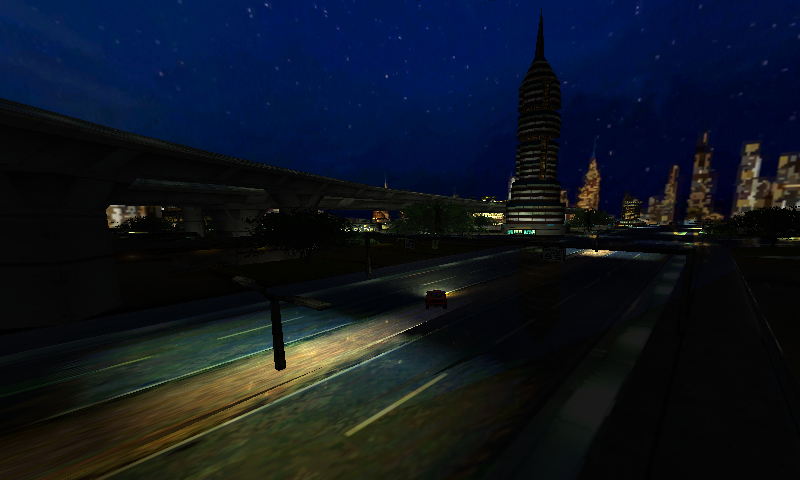
\includegraphics[width=120mm]{figures/lamps.png}
\caption{Scéna s aplikovanými mapami osvětlení lamp}
\end{center}
\end{figure}

\subsection{Vytváření map osvětlení}
Vytváření map osvětlení je realizováno dvěma přístupy, prvním je rasterizační (pomocí OpenGL) a druhým je vrhání paprsku. Pro rasterizační přistup jsou k dispozici dva druhy světel: bodové světlo a reflektor. Tyto světla jsou definovaná přímo v 3D modelovacím software. Dosah světel je omezen na 300metrů (je to z důvodu chyb, které vznikají u osvětlení\linebreak na velkou vzdálenost). Světla pochopitelně nepoužívají spekulární složku, protože tato složka je závislá na pohledu kamery a tudíž jí nelze předpočítat.

I maximální možné rozlišení map osvětlení pro použitou scénu není dostatečné a stíny jsou kostičkované. Z tohoto důvodu se používají dva druhy filtrování. Prvním je rozmazání map osvětlení, které se provádí přímo po generování mapy osvětlení a druhým je lineární filtrování, které se aplikuje až při aplikování mapy osvětlení. Tato kombinace filtrování značně zvýší výslednou kvalitu stínů.

V přístupu využívající vrhání paprsku jsou navíc k dispozici plošné zdroje světla, které jsou definovány pomocí osvětlovacích textur, což jsou textury, u kterých jsou vykresleny pouze texely vyzařující světlo. Osvětlovací textury mají stejné texturovací souřadnice jako difúzní textury 3D modelu. Plošný zdroj světla se realizuje tak, že každý barevný texel\linebreak v osvětlovací textuře vygeneruje bodový zdroj světla. Množina vzniklých bodových světel pak tvoří plošný zdroj světla.

\begin{figure}[h]
\begin{center}$
\begin{array}{cc}
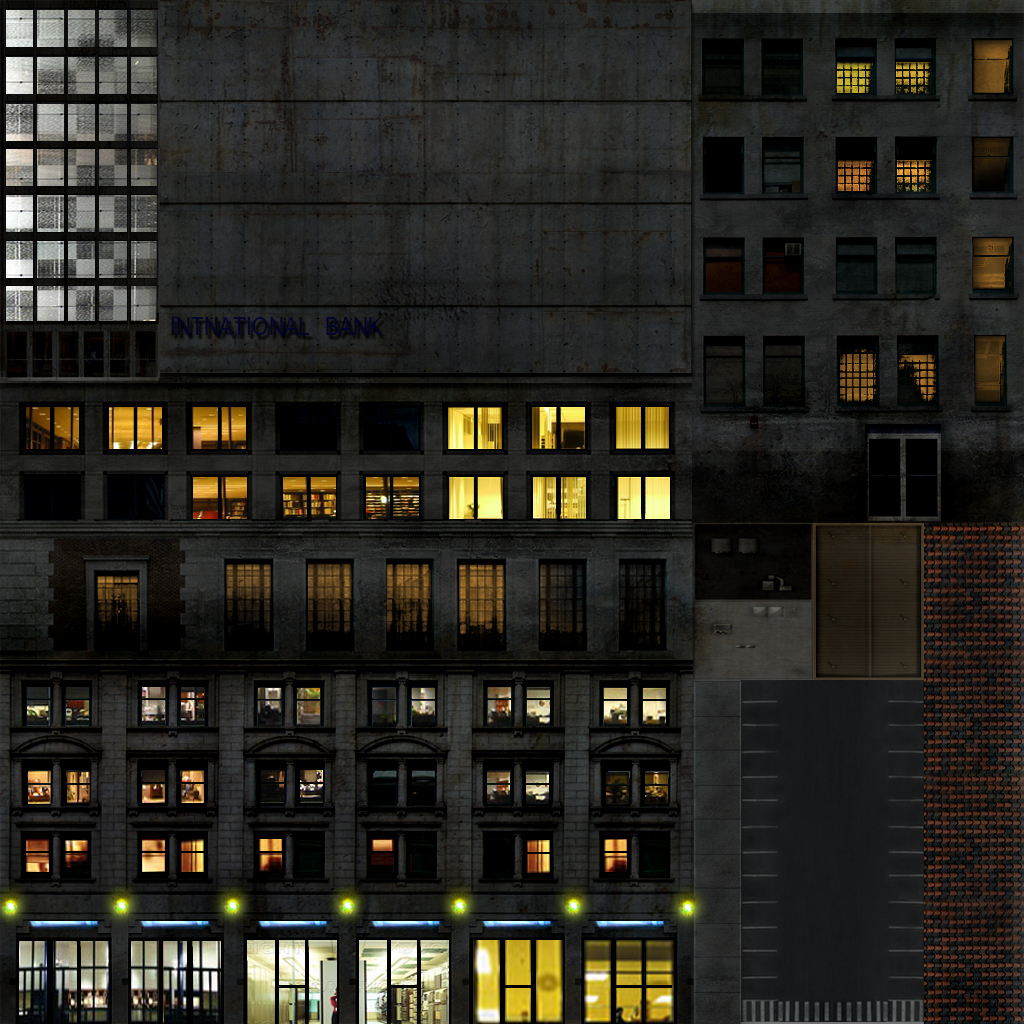
\includegraphics[width=70mm]{figures/buildz3-n.png} &
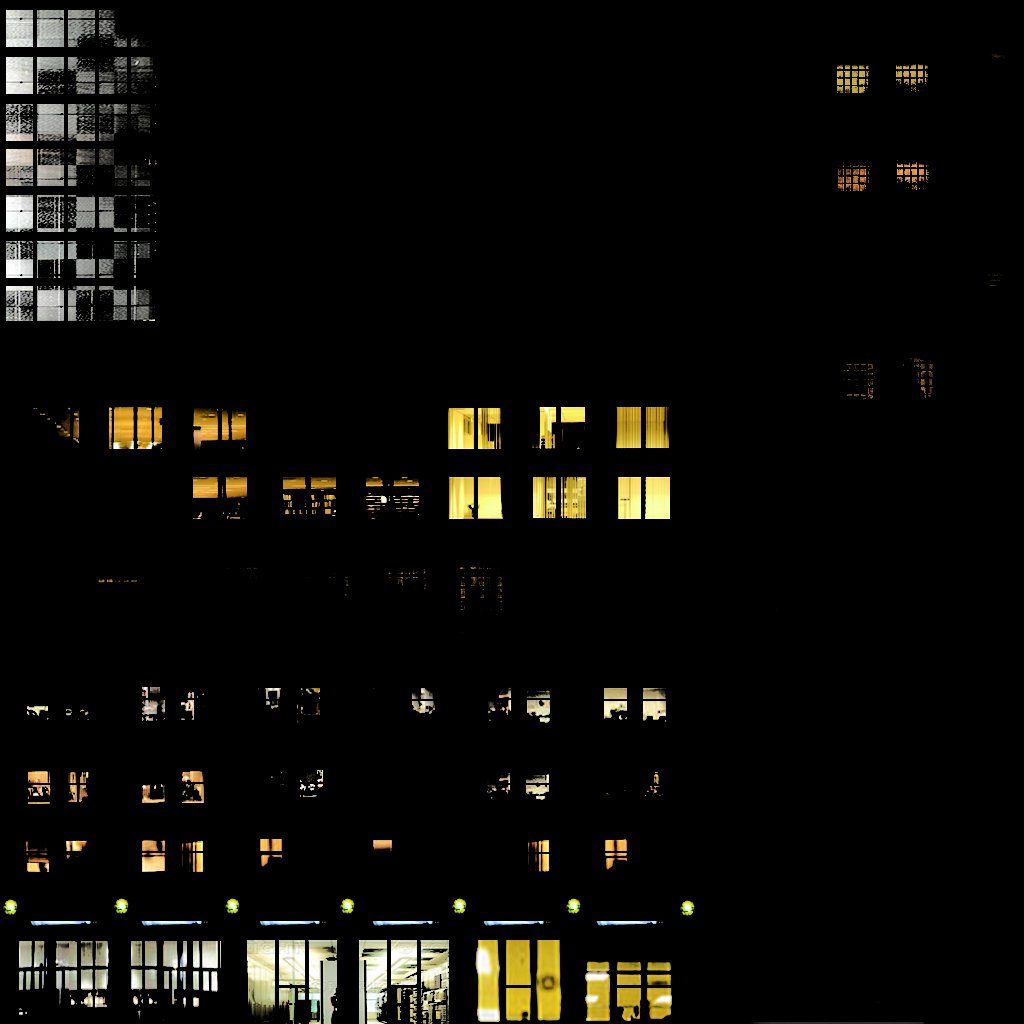
\includegraphics[width=70mm]{figures/buildz3-e.png}
\end{array}$
\end{center}
\caption{Ukázka difúzní textury modelu (vlevo) a osvětlovací textury (vpravo)}
\end{figure}

V obou přístupech je výsledná mapa osvětlení 24-bitová RGB bitmapa uložená ve formátu PNG. Formát PNG zajišťuje bezztrátovou kompresi bitmapy.
\newpage

\subsection{Generování texturovacích souřadnic pro mapy osvětlení}
V teoretické části byl popsán postup generování texturovacích souřadnic pomocí ILP.\linebreak V praxi toto řešení nelze použít, protože jeho výpočetní složitost metody je $O(m^2 \cdot n^2)$, kde $m$ je počet trojúhelníků a $n$ počet texelů v lightmapě.  Pomocí ILP se tedy dají řešit pouze velice malé instance problému. V této práci problém řeším pomocí metody Packing Lightmaps \cite{Scott02}, což je metoda řešící problém batohu za použití datové struktury kD stromu, která dělí $k$-rozměrný objekt půlením.

V případě Packing Lightmaps dělíme rovinu horizontálním nebo vertikálním řezem. kD strom je typ binárního stromu, jehož kořen reprezentuje k-rozměrný objekt (v našem případě mapu osvětlení). Vnitřní uzly jsou dělící, určují podle které osy se provede řez a je v nich zapsána také pozice řezu. Listy stromu reprezentují objekty uložené ve struktuře, v mém případě AABB - tedy dva párové trojúhelníky (viz kapitola 4.2).

\begin{center}
\begin{figure}[h]
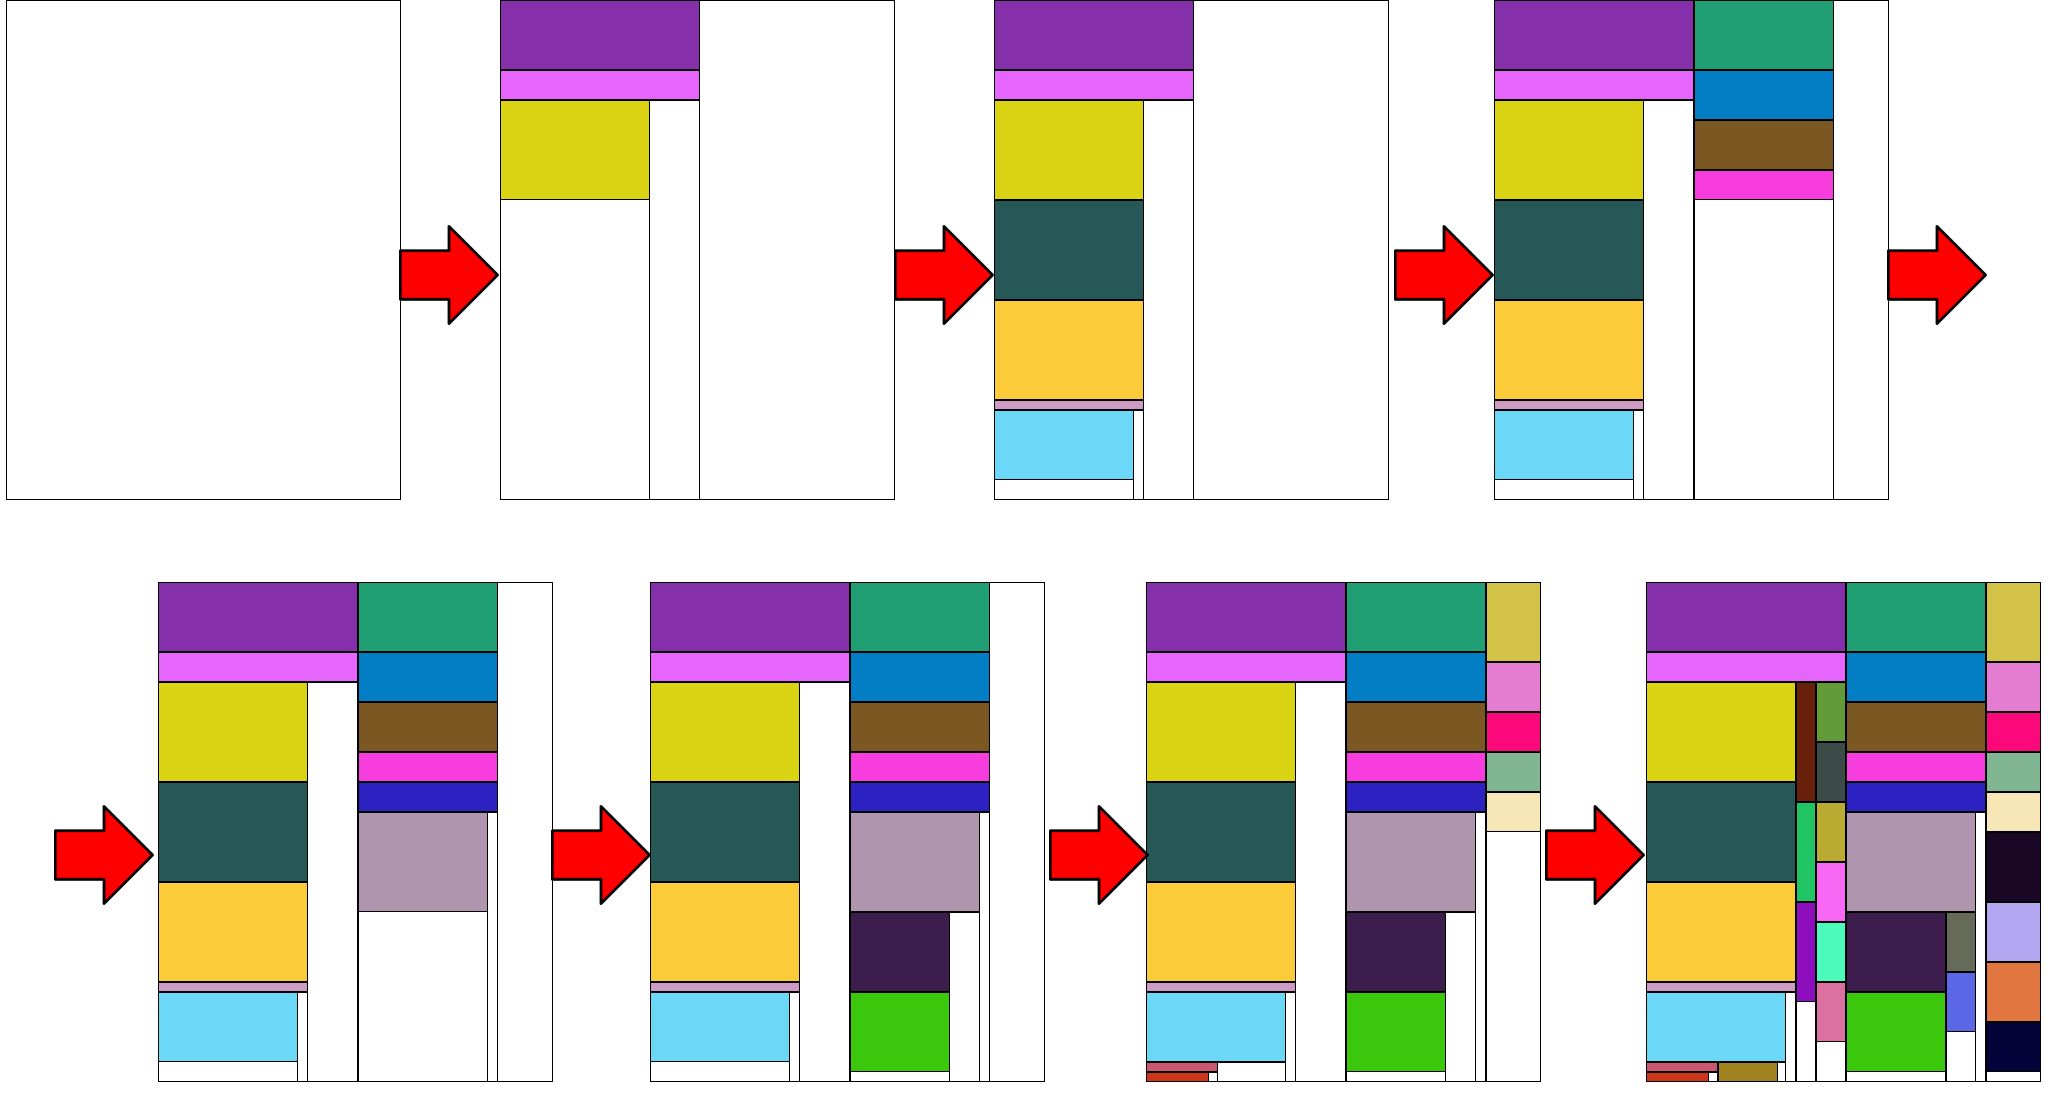
\includegraphics[width=120mm]{figures/kd.png}
\caption{Ukázka naplnění kD stromu pomocí metody Packing Lightmaps}
\end{figure}
\end{center}

Metoda Packing Lightmaps nejdříve seřadí AABB podle jejich plochy a postupně je vkládá do kD stromu. Při každém vložení se nejdříve hledají neobsazené listy, zda neexistuje takový, který by odpovídal rozměrům AABB. Pokud takový neexistuje, pokusí se algoritmus nalézt takový neobsazený list, kterému odpovídá aspoň jeden rozměr. V případě úspěšného hledání se AABB vloží do listu, v ostatních případech se najde větší list, provede se jeho rozdělení a následně se AABB do jednoho z potomků vloží.
\newpage

\lstset{language=Java} 
\begin{lstlisting}[caption=Vkládání AABB do kD stromu za využití rekurze]
public boolean addAABB(AABB aabb) {
  // check if current node is empty and has enought space for AABB
  if (isEmpty() && (aabb.width <= width) && (aabb.height <= height)) {
    // fits exactly
    if ((aabb.width == width) && (aabb.height == height)) {
      child1 = new KDNode(aabb);
      return true;
    }         
    // subdivision
    else {
      child1 = new KDNode(aabb.width, height);
      if (child1.addAABB(aabb))
        return true;
    }
  }     
  // try to insert into first child
  else if (child1.addAABB(aabb))
    return true;

  // create second child
  else if (child2 == null) {    
    // horizontal subdivision
    if ((aabb.width <= width) && (aabb.height <= getChild2Height())) {
      child2 = new KDNode(width, height - aabb.height);
      if (child2.addAABB(aabb))
        return true;
    }      
    // vertical subdivision
    if ((aabb.width <= getChild2Width()) && (aabb.height <= height)) {
      child2 = new KDNode(width - child1.width, height);
      if (child2.addAABB(aabb))
        return true;
    }
  }     
  // try to insert into second child
  else if (child2.addAABB(aabb))
    return true;
  return false;
}
\end{lstlisting}

\subsection{Generování map osvětlení}
Generování map osvětlení znamená v podstatě vykreslení celé scény v souřadnicích map osvětlení (tím se vykreslí celá scéna, aniž by docházelo k zakrývání objektů). Generování je\linebreak v práci řešeno dvěma různými přístupy. Prvním přístupem je rasterizační (pomocí OpenGL) a druhým je vrhání paprsku. V obou přístupech se provede výpočet difúzního osvětlení stejným způsobem jako se provádí při běžném vykreslování scény. 

Aby mapa osvětlení obsahovala stíny, musí se provést test viditelnosti jednotlivých bodů pro jednotlivá světla. V rasterizačním přístupu se toto provádí pomocí stínových map (viz. kapitola 4.3).

V druhém přístupu se pro každý zdroj světla vrhají paprsky do všech bodů v mapě osvětlení (paprsky mají definováno, kde končí). Pokud paprsek protne mezi počátkem\linebreak a destinací nějaký trojúhelník, nepřipočte se pro bod v osvětlovací mapě příspěvek z daného zdroje světla.

Pokud bychom testovali pro každý paprsek existenci průsečíku s nějakým trojúhelníkem ve scéně, bylo by generování příliš pomalé. Z toho důvodu jsem použil akcelerační datovou strukturu octree. Octree je stromová datová struktura, která dělí rovnoměrně prostor vždy na osm stejných podprostorů. V mé realizaci každý uzel určený pomocí AABB a seznamu trojúhelníků, který do AABB spadají.

Stavba stromu octree se provádí odshora dolů, to znamená, že nejdříve se všechny trojúhelníky vloží do kořenového uzlu a po té se provede jejich přesun do nižších uzlů, pokud jsou splněna následující kritéria.
\begin{itemize}
\item dochází k průniku AABB trojúhelníka a AABB aktuálního uzlu
\item počet trojúhelníků v aktuálním uzlu je vyšší než 20 (v takovém případě je neefektivní strom dále větvit)
\end{itemize}

\lstset{language=C++} 
\begin{lstlisting}[caption=Průnik dvou AABB ve 3D]
bool TestAABBAABB(AABB* a, AABB* b) {
    if (a->max[0] < b->min[0] || a->min[0] > b->max[0]) return false;
    if (a->max[1] < b->min[1] || a->min[1] > b->max[1]) return false;
    if (a->max[2] < b->min[2] || a->min[2] > b->max[2]) return false;
    return true;
}
\end{lstlisting}

Po sestavení stromu máme tedy rozdělené trojúhelníky do segmentů, které jsou definované pomocí AABB. Abychom nalezli průsečík paprsku s nějakým trojúhelníkem ve scéně, musíme strom procházet. Nejdříve provedeme test průniku paprsku s AABB potomků kořene. U každého potomka, u kterého byl test pozitivní, provedeme test jeho potomků. Tímto způsobem pokračujeme dokud se nedostaneme na úroveň listů. V každém uzlu, u kterého byl test pozitivní, provedeme také test průsečíku se všemi trojúhelníky, které má v seznamu. Pokud test jakéhokoliv trojúhelníku je pozitivní, vrátíme test paprsku jako pozitivní.

Ukázka rekurzivního hledání v octree je na obrázku 5.4 (na obrázku je pouze quadtree, což je obdoba octree ve 2D).

\begin{center}
\begin{figure}[h]
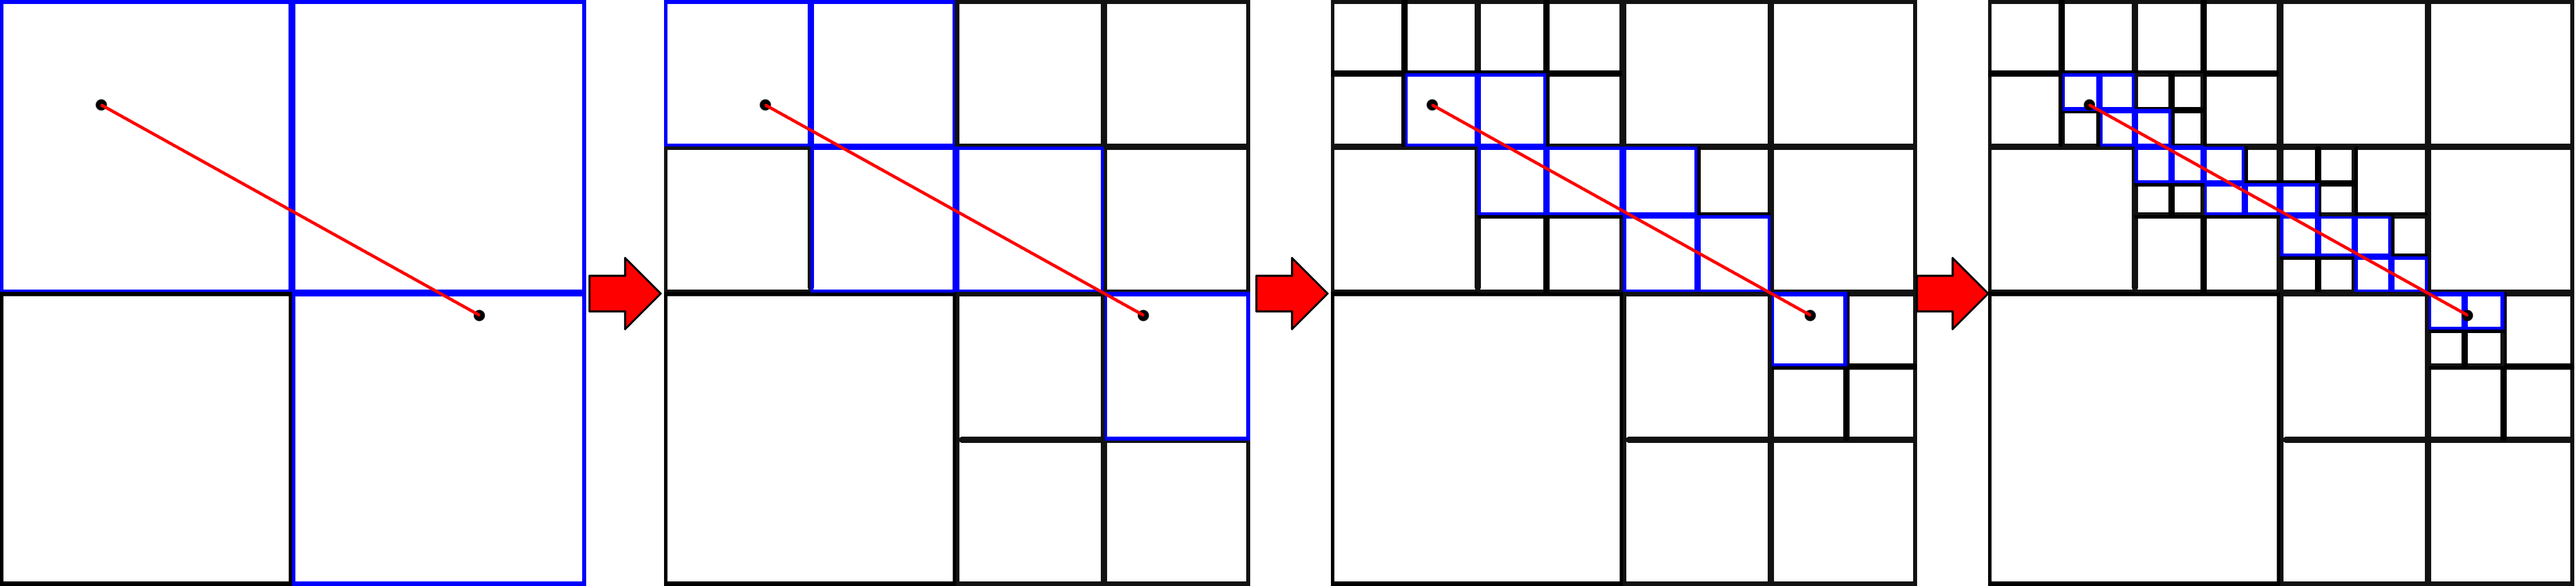
\includegraphics[width=150mm]{figures/quadtree.png}
\caption{Ukázka hledání průsečíku paprsku v datové struktuře quadtree}
\end{figure}
\end{center}

Aby hledání ve stromu bylo ještě rychlejší, lze použít ještě několik optimalizací. Může se například ukládat $n$ posledních průsečíků a testovat, jestli další paprsek nemá stejný průsečík se stejným trojúhelníkem jako předešlý paprsek. Tato optimalizace má smysl pouze pro malé $n$. V mém projektu jsem nastavil $n = 2$. Paprsky testuji v pořadí podle indexu cílového trojúhelníku.

Dále je vhodné přeskakovat testy stejných trojúhelníků. Podle zvoleného kritéria dělení stromu při jeho stavbě může dojít k tomu, že některé trojúhelníky jsou uloženy ve stromu ve více uzlech (pokud AABB trojúhelníku náleží více uzlům stejné hloubky). Řešit to lze jednoduše. Stačí si u trojúhelníku vždy pamatovat ID paprsku, s kterým byl proveden poslední test průsečíku. Díky tomu lze zjistit, jestli některý paprsek není testován víckrát a případně tento test přeskočit. Této optimalizaci se říká mailboxing technika.

Další možnost urychlení generování map osvětlení je přeskakování testování paprsků,\linebreak u kterých je délka paprsku delší než vzdálenost, na kterou dosvítí zdroj světla. Tuto vzdálenost lze spočítat pomocí vzorce pro útlum (viz. kapitola 3.2). Minimální přípustnou hodnotu si označím $\epsilon$ a maximálně délku paprsku jako $d$.
\begin{center}
$F_a = \frac{1}{k_c + k_l \cdot d + k_q \cdot d^2}$, $F_a = \epsilon$
\end{center}
Po dosazení a otočení rovnice získáme výraz
\begin{center}
$k_c + k_l \cdot d + k_q \cdot d^2 = \frac{1}{\epsilon}$
\end{center}
Vzdálenost $d$ spočteme pomocí diskriminantu
\begin{center}
$D = {k_l}^2 - 4 \cdot k_q \cdot (k_c - \frac{1}{\epsilon})$\\
$d = \frac{-k_l \pm \sqrt{D}}{2 \cdot (k_c - \frac{1}{\epsilon})}$
\end{center}


\paragraph{Akumulace výsledků}\ \ \\

Výsledky od jednotlivých statických zdrojů světel se sčítají do jedné skupiny map osvětlení a provádí se ořez maximální hodnoty barvy, aby nedocházelo k přetečení hodnoty.\linebreak U všech příspěvků se zapisuje pouze $1/8$ jeho hodnoty, je to z důvodu potřeby rozšíření rozsahu intenzity světla. 

U plošných zdrojů světel se provádí vzorkování na bodové zdroje světla. Vzorkování se provádí tak, aby každý vzniklý bodový zdroj odpovídal jednomu texelu v mapě osvětlení.\linebreak Z toho důvodu je třeba při změně cílového rozlišení mapy osvětlení změnit i parametr intenzity vygenerovaných bodových zdrojů světel, aby pro různé rozlišení nebyla scéna osvětlena jinak.

U dynamických zdrojů světel se provádí pro každé světlo vykreslení skupiny map osvětlení, ty se zkomprimují do vektorové podoby a pro další dynamický zdroj světla se použije opět nová skupina map osvětlení. Jednotlivé dynamické zdroje světla nejsou na sobě tedy závislé.

\subsection{Příprava dat pro dynamickou aktualizaci map osvětlení}
Data pro dynamickou aktualizaci map osvětlení se nazývají záplaty. Záplata je v podstatě také mapa osvětlení, ale pouze pro jeden zdroj světla. Problém je, že tyto záplaty by byly příliš paměťově náročné, proto používám vektorovou podobu těchto dat.

Data záplaty jsou při běhu testovací aplikace uloženy jako trojúhelníky ve VBO (tedy na GPU). Každý vrchol má dva atributy a to pozici v mapě osvětlení a barvu světla vynásobenou intenzitou. Lze tedy snadno a rychle mapy osvětlení aktualizovat, pokud máme záplaty v této podobě uloženy.

Abychom získali záplaty v této podobě musíme nejdříve pro každý dynamický zdroj světla vykreslit mapu osvětlení a poté tyto data zvektorizovat. Pro zvektorizování lze využít informaci o souřadnicích jednotlivých trojúhelníků v mapě osvětlení. Pokud barycentricky interpolujeme barvu světla z vrcholů trojúhelníku, měla by odpovídat barvě uložené v map osvětlení $lm$. 

Pro $\forall$ body $p$ náležící trojúhelníku, lze ověřit interpolaci barvy ve vrcholech $a$, $b$ a $c$ pokud známe barycentrické váhy $Wp$ pro body $p$ níže uvedeným vzorcem ($\epsilon$ je tolerance odchylky barvy).
\begin{center}
$I_k = lm[p_u][p_v]$\\
$I_l = Wp_a \cdot lm[a_u][a_v] + Wp_b \cdot lm[b_u][b_v] + Wp_c \cdot lm[c_u][c_v]$\\
$|I_k - I_l| < \epsilon$
\end{center}

Pokud byl test úspěšný, přidá se geometrie trojúhelníku do vektorových dat záplaty. Pokud ne, rozdělí se trojúhelník na čtyři menší trojúhelníky a znovu se provádí testování (viz. obrázek 5.5).

\begin{center}
\begin{figure}[h]
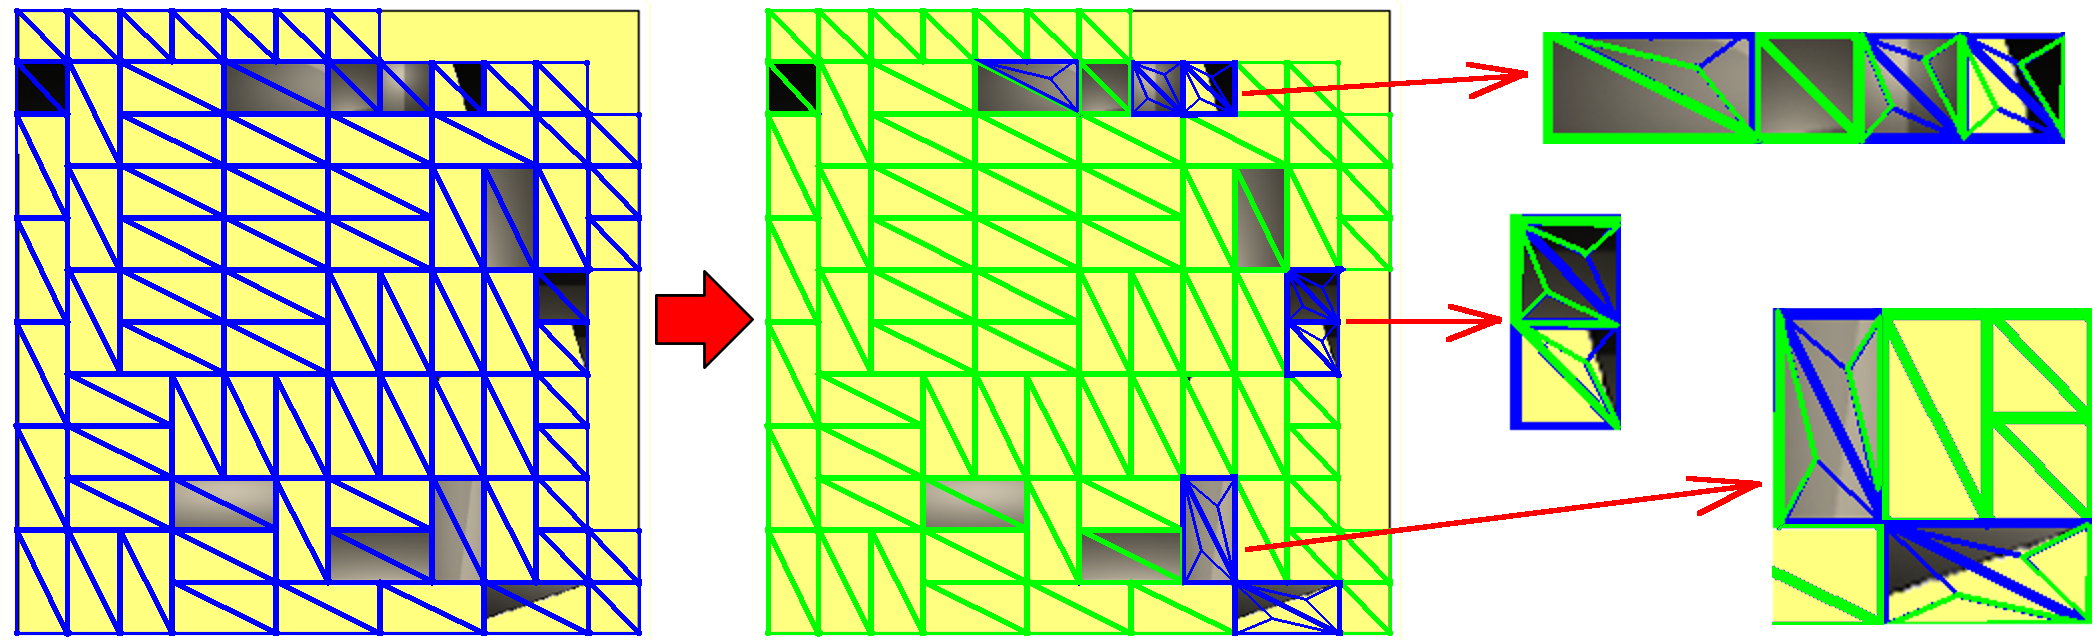
\includegraphics[width=150mm]{figures/lmpatch.png}
\caption{Ukázka převodu záplaty osvětlovací mapy do vektorové podoby, vlevo původní mapa osvětlení, uprostřed první iterace algoritmu a vpravo další iterace}
\end{figure}
\end{center}
\newpage

\section{Testovací aplikace - simulátor}
Simulátor je navržen tak, aby fungoval na X11-Linuxu a Androidu. Znamená to výběr multiplatformních knihoven nebo ve výjimečných případech rozdílných implementací pro jednotlivé platformy. K vykreslování jsem vybral OpenGL ES 2.0 (jedná se o odlehčené OpenGL 3.0) a GLSL core verzi 1.0 (to zaručuje maximální možnou kompatibilitu).

Fyzikální vlastnosti vozidel jsou realizovány pomocí enginu Bullet Physics (tento engine používá mnoho známých firem zabývajících se vývojem mobilních her). Zvuk je realizován na mobilních zařízeních pomocí Android API a na Linuxu pomocí knihovny FMOD API. Správce oken je na Androidu třeba doprogramovat, aby fungovalo dotykové ovládání a pozastavení simulátoru (např. při hovoru). Na Linuxu je použitá knihovna freeglut.

Samotný simulátor je rozdělen do dvou oddělených částí. První část je abstraktní\linebreak a řeší logickou část projektu. Abstrakce je realizována pomocí rozhraní, které definují společné metody abstraktních objektů. Druhá část implementuje jednotlivá rozhraní a řeší také načítání dat ze souborů.
\lstset{language=C++} 
\begin{lstlisting}[caption=Načtení 3D modelu vozidla pomocí abstraktního přístupu]
    /// load models
    skin = getModel(getConfigStr("skin_model", atributes), false);
    wheel = getModel(getConfigStr("wheel_model", atributes), false);

    /// set car wheels position
    wheelX = getConfig("wheel_x", atributes);
    wheelY = getConfig("wheel_y", atributes);
    wheelZ1 = getConfig("wheel_back", atributes);
    wheelZ2 = getConfig("wheel_front", atributes);
\end{lstlisting}

Důvodem oddělení částí je, že implementace jednotlivých rozhraní může být v budoucnu snadno nahrazena anebo mohou být použité různé implementace pro různé platformy. Příkladem různých implementací rozhraní pro různé platformy může být například renderer.\linebreak V simulátoru je využita knihovna OpenGL, která například na platformě Windows Phone není dostupná a bylo by potřeba na této platformě použit Direct3D.
\newpage

\begin{figure}[h]
\begin{center}
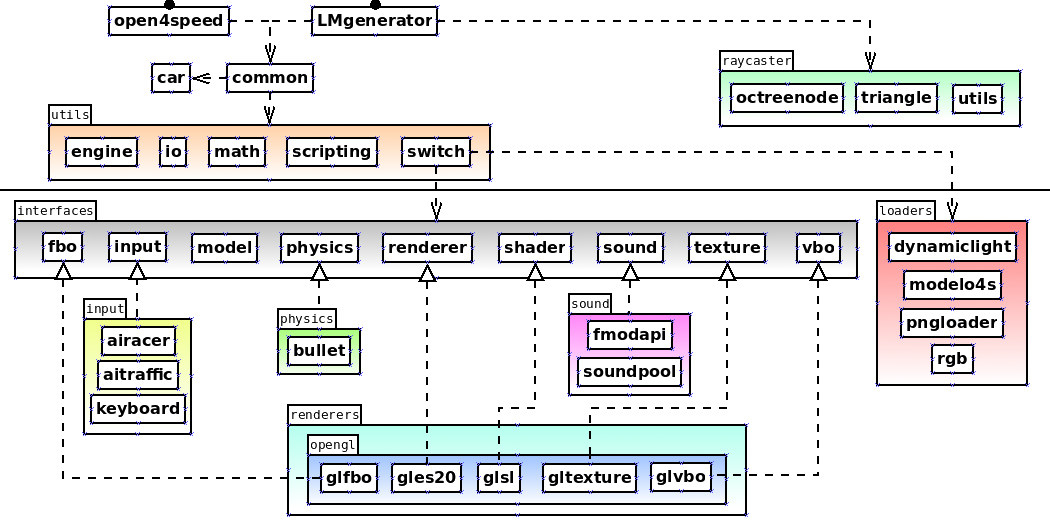
\includegraphics[width=160mm]{figures/o4suml.png}
\caption{UML diagram projektu, horní část je abstraktní, dolní část implementuje jednotlivá rozhraní a načítá data do paměti, spustitelné soubory jsou označeny tečkou}
\end{center}
\end{figure}
Jak je vidět na obrázku 5.6, simulátor je rozdělen do dalších dílčích částí. Část \ul{raycaster} a třída \ul{LMgenerator} realizují předzpracování. Třída \ul{open4speed} se zabývá správou okna\linebreak a spouštění dílčích součástí. \ul{Common} uchovává veškeré objekty a proměnné, je to z důvodu, že jinak by v třídách \ul{open4speed} a \ul{LMgenerator} musel být obsah struktury \ul{common} duplicitně.

Třída \ul{car} je v první řadě struktura uchovávající veškeré proměnné realizující vozidlo, dále zajišťuje propojení mezi fyzikálním enginem, vykreslováním, zvukem, vstupem umělé inteligence a uživatele.
\\ \\
Část \ul{utils} je balík příkazů tvořící simulátor.
\begin{itemize}
\item \ul{engine} realizuje GUI a 3D scénu
\item \ul{io} obstarává práci se soubory
\item \ul{math} poskytuje sadu matematických příkazů pro práci s 3D objekty
\item \ul{scripting} interpretuje skriptování GUI
\item \ul{switch} obstarává objekty jednotlivých rozhraní a naplňuje je daty
\end{itemize}

Jednotlivá rozhraní mají různé funkce. Rozhraní \ul{fbo}, \ul{renderer}, \ul{shader}, \ul{texture} a \ul{vbo} vytváří abstraktní přístup k OpenGL, \ul{input} je rozhraní pro ovládání vozidla (implementací může být buď klávesnice anebo umělá inteligence), rozhraní \ul{physics} reprezentuje fyzikální engine a rozhraní \ul{sound} umožňuje přehrávat zvuky. Implementace rozhraní \ul{sound} jsou příkladem použití různých implementací na různých platformách.

\section{Realizace na platformě Android}
Platforma Android je postavená na Linuxovém jádře a využívá mnohé komponenty\linebreak z projektu GNU, nicméně celé Android API je v jazyku Java za využiti virtuálního stroje Dalwik. Pomocí Android NDK(native development kit) je možné zkompilovat C/C++ kód jako knihovnu, kterou je možné zavolat z jazyku Java. Toto je prováděno pomocí JNI(Java native interface).

\begin{center}
\begin{figure}[h!]
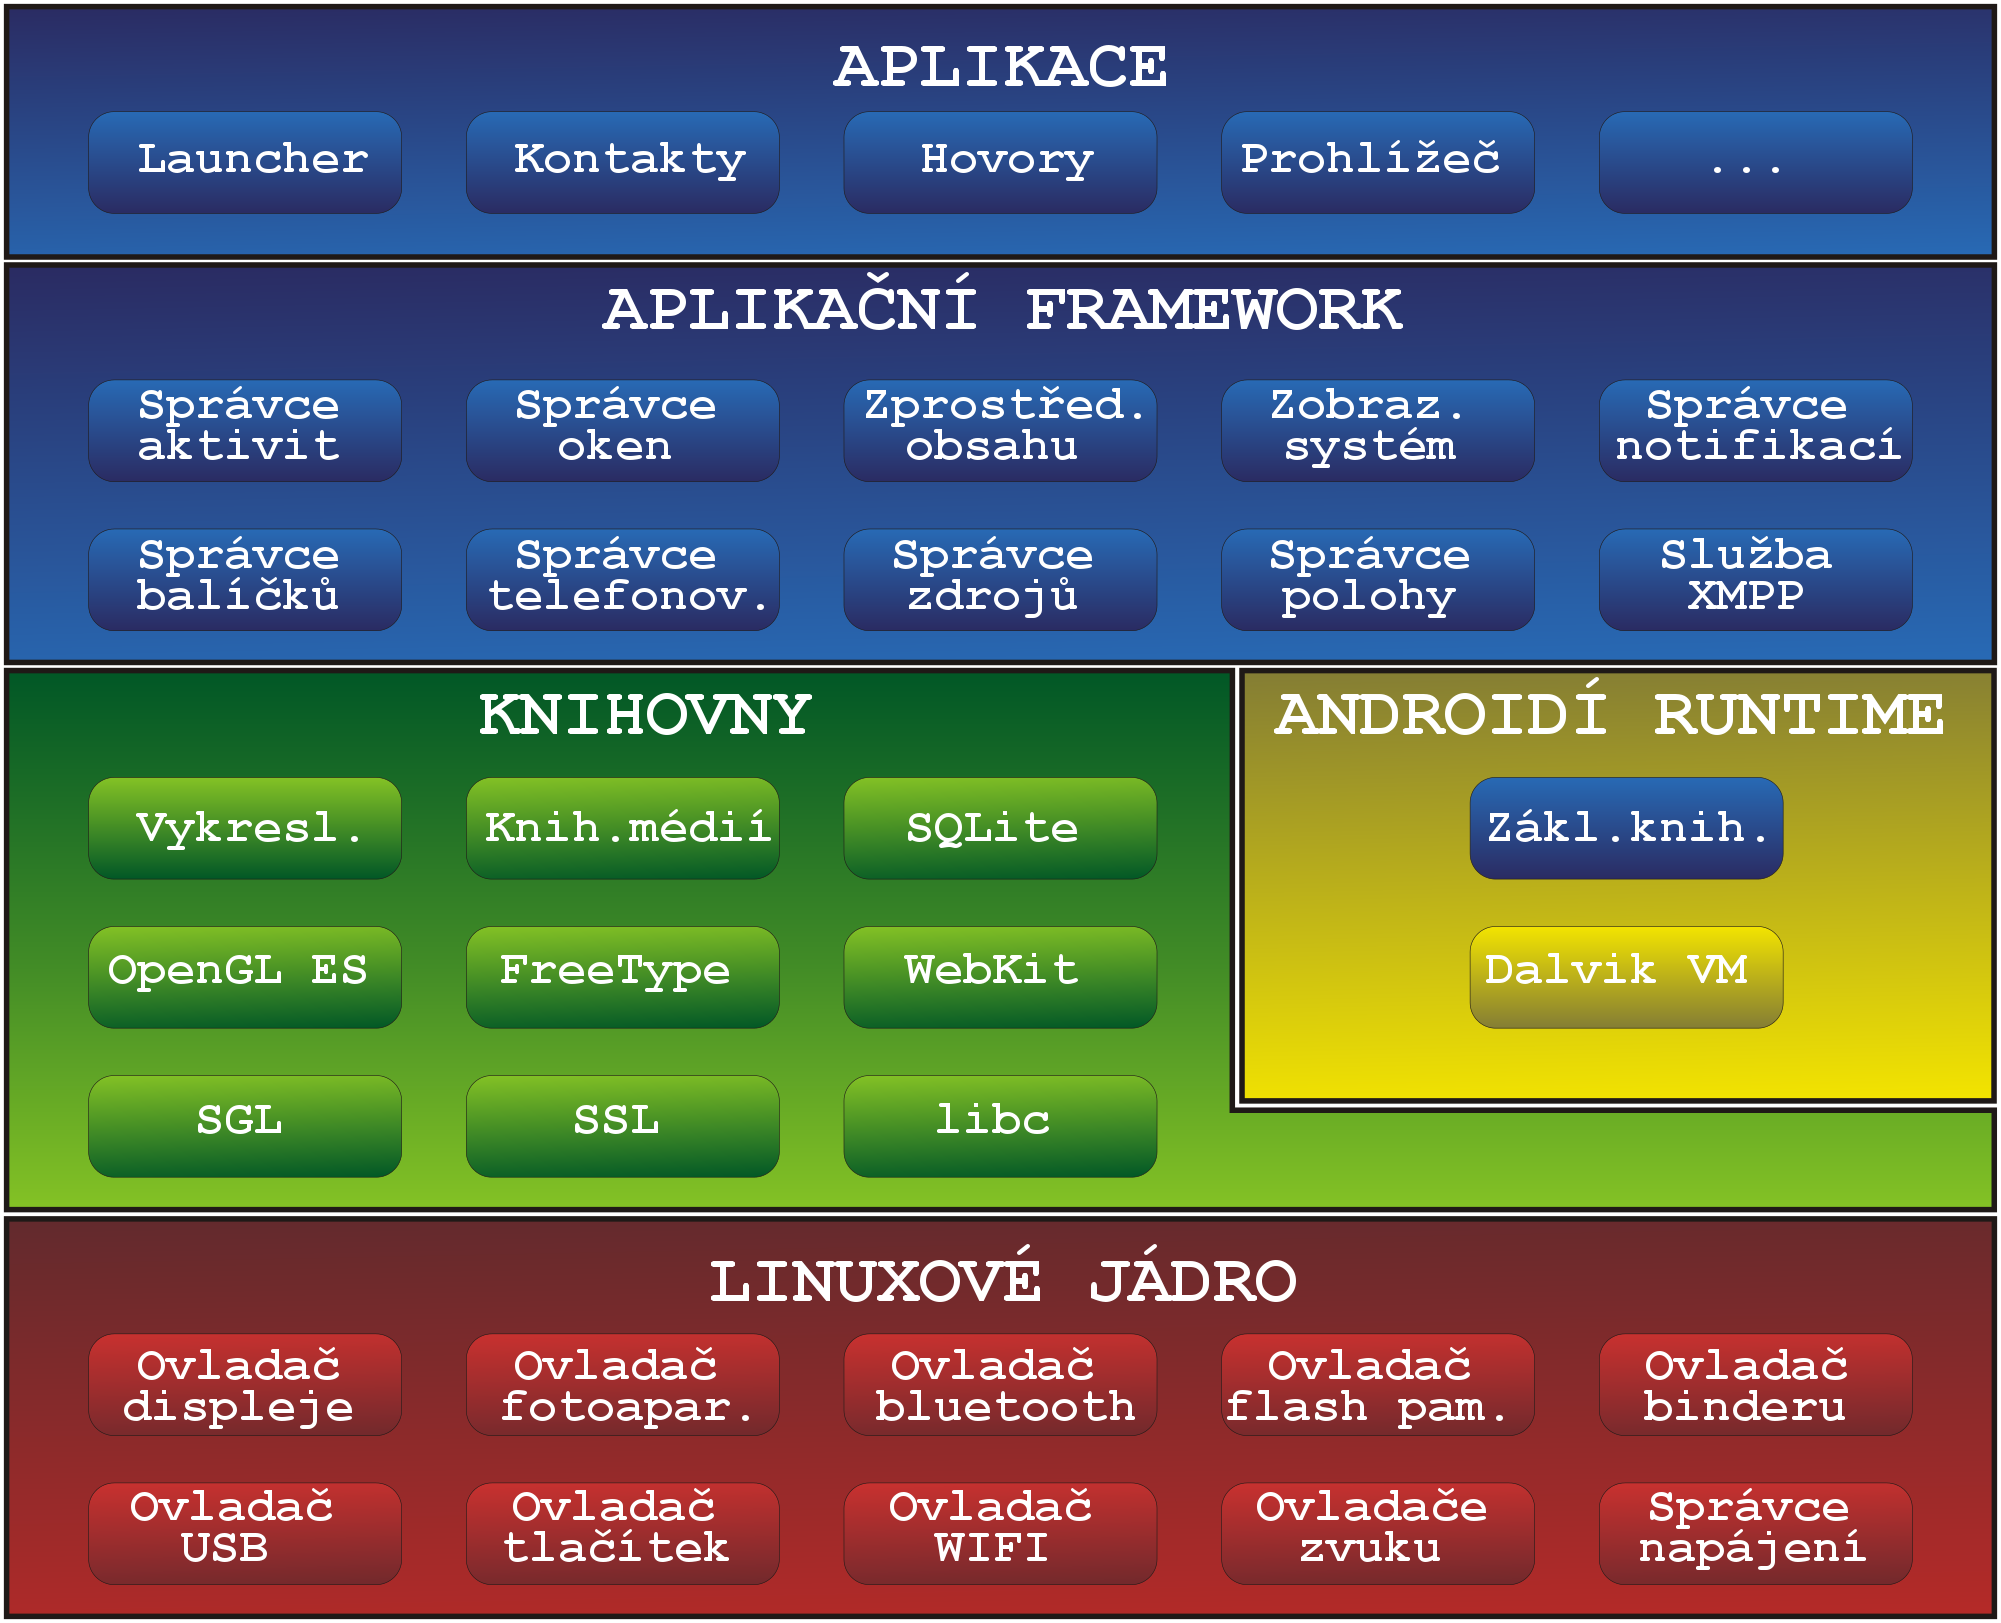
\includegraphics[width=120mm]{figures/android.png}
\caption{Komponenty platformy Android, komponenty vyznačené modrou barvou jsou napsané v jazyce Java, žlutou barvou je virtuální stroj, který umožňuje běh Java aplikací, zelenou barvou jsou C/C++ knihovny a červenou je Linuxové jádro}
\end{figure}
\end{center}

Snažší by bylo naprogramovat simulátor přímo v Javě, ale tím bych ztratil možnost portovat simulátor na další platformy, které virtuální stroj Dalwik nemají. Dále by byl problém s použitím fyzikálního enginu, který je napsaný v jazyce C++. Musel bych napsat interface pro fyzikální engine, který by mi umožnil komunikaci mezi C++ a Java kódem.

\subsection{Problematika Android API}
Java native interface je rozhraní, které umožňuje spustit C++ kód z jazyku Java a obráceně. Největší problém je, že neexistuje použitelný port freeglut knihovny pro Android. Udělal jsem tedy JNI rozhraní, které odpovídá handlerům knihovny freeglut. Tedy nahrazuji veškeré funkce této knihovny svou implementací. Knihovna implementuje správu oken, vstup klávesnice a myši a volání idle a display funkcí. Klávesnice a myš byla pochopitelně plně nahrazena dotykovým ovládáním, ale pokud do Android zařízení připojíme klávesnici nebo myš, bude plně funkční. Funkčnost myši zařizuje sám systém, klávesnice stačila namapovat.

Aby bylo možné volat C++ metody přímo z Javy musí být pojmenovány ve formátu Java\_\textit{package}\_\textit{třída}\_\textit{metoda}. C++ knihovna bude tedy možné spustit pouze z jedné Java třídy.
\lstset{language=C++} 
\begin{lstlisting}[caption=Volání metod pomocí JNI v C++ pro nahrazení freeglut knihovny]
void Java_com_cvut_o4s_O4SJNI_nativeInit(JNIEnv* e) { main(0, 0); }
void Java_com_cvut_o4s_O4SJNI_nativeKey(JNIEnv* e, jint i) { key(i); }
void Java_com_cvut_o4s_O4SJNI_nativeDisplay(JNIEnv* e) { display(); }
\end{lstlisting}

Dále je potřeba C++ knihovnu načíst pomocí volání System.loadLibrary a metody deklarovat v dané Java třídě pomocí klíčového slova native.

\lstset{language=Java} 
\begin{lstlisting}[caption=Ukázka deklarování C++ metod v Java kódu]
static native void nativeInit();
static native void nativeKey(int i);
static native void nativeDisplay();
\end{lstlisting}

Dalším problémem je volání Android API z C++ kódu (tzn. volání Java kódu z C++). Příkladem je přehrávání zvuků pomocí Android API, ovládání zvuku je nutno řídit z C++, ale API je přímo přístupné pouze z Javy. Na obrázku 5.8 je znázorněn případ třídy Sounds. Problém se řeší také pomocí JNI, pouze volání jsou prováděny v opačném směru.

\begin{center}
\begin{figure}[h]
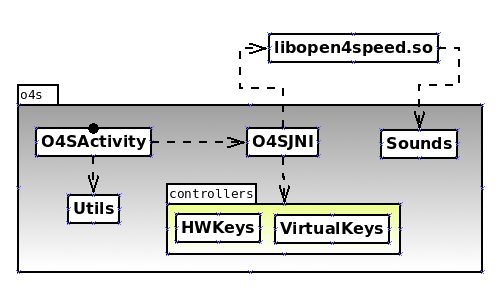
\includegraphics[width=80mm]{figures/jni.png}
\caption{UML diagram spustitelného klienta pro Android, kde libopen4speed.so je zkompilovaná C++ knihovna projektu}
\end{figure}
\end{center}

\lstset{language=C++} 
\begin{lstlisting}[caption=Volání Java metody pro přehrání zvuku z C++ kódu]
void soundpool::play(int index) {
  jclass clazz = instance->FindClass("com/cvut/o4s/Sounds");
  //get method "void soundPlay(int, int)"
  jmethodID method = instance->GetStaticMethodID(clazz, "soundPlay", "(II)V");
  instance->CallStaticVoidMethod(clazz, method, index, (int)looping);
}
\end{lstlisting}

V Javě se poté musí ještě rozlišovat přehrávání zvuků od přehrávání hudby. Hudba bývá řádově náročnější na paměť a nemá smysl jí celou držet v paměti, když na ni není potřeba aplikovat další zvukové efekty.

\lstset{language=Java} 
\begin{lstlisting}[caption=Přehrání zvuku v Javě pomocí Android API]  
public static void soundPlay(int index, int loop) {
  //instance is a music
  if (list.get(index).id == TYPE_MUSIC) {
    music.setLooping(loop == 1);
    music.start();
  }

  //audio clip
  else {
    Sound s = list.get(index);
    snd.play(s.id, s.volume, s.volume, 1, loop, s.rate);
  }
}
\end{lstlisting}

\subsection{Využití vláken}
Většina zařízení, které dnes už spadají do střední třídy, je vybavena alespoň dvěma procesory, je proto vhodné rozdělit činnost do více vláken, aby bylo dosaženo maximálního výkonu. Třída GLSurfaceView, která umožňuje vykreslovat OpenGL scénu z C++ umožňuje volat OpenGL příkazy pouze z jednoho vlákna. Z tohoto důvodu jsem rozdělil kód na grafické\linebreak a negrafické vlákno.

V menu simulátoru se používá pouze grafické vlákno, negrafické vlákno je primárně použito pro fyzikální výpočty, které zařízení vytěžují nejvíce. Vlákna jsou synchronizovaná, aby nedocházelo k použití transformace vozidla z předešlého snímku(to by bylo velmi rušivé).

Dále provádím regulaci rychlosti simulátoru v závislosti na výkonu hardwaru. Je potřeba, aby obě vlákna prováděla výpočet co nejvíce paralelně, pokud by negrafické vlákno příliš dlouho nedodávalo novou transformaci vozidla, docházelo by k trhanému vykreslování (některý snímek by se vykresloval víckrát a to by se projevilo tak, že by se snímková frekvence zdála být na krátký okamžik poloviční). Pokud k tomuto případu dojde, je vhodné snížit frekvenci volání obou vláken a tím snížit rychlost simulátoru.

Problém je, že nelze snižovat rychlost simulátoru do nekonečna, proto je zde nastavena minimální hodnota, na kterou se může simulátor zpomalit. Je zde i horní limit, aby nedocházelo k zrychlené jízdě a tedy i ke zvýšené spotřebě energie.

\subsection{Práce se soubory}
V Androidu se aplikace publikují v APK balíčku. Jedná se o ZIP soubor, který má nějakou danou strukturu. V Java kódu je možné na veškeré soubory uvnitř balíčku přistupovat,\linebreak v C++ tato možnost není. Někteří vývojáři toto řeší, že po prvním spuštění si aplikace stáhne ze serveru přídavná data a ty si uloží například na paměťovou kartu. Lze také rozbalit soubory z APK balíčku a s těmi pak v C++ pracovat. To se moc nepoužívá, protože jsou potom data v zařízení dvakrát.

Další možnou variantou je přistupovat k APK balíčku jako k ZIP souboru. Knihovna libZIP umožňuje zpracovávat data ze ZIP souboru jako kdyby byla uložena normálně na disku nebo na paměťové kartě. To má výhodu, že data jsou komprimovaná a zároveň přístupná.
\lstset{language=C++} 
\begin{lstlisting}[caption=Čtení řádky z APK balíčku (vlevo) a ze souboru (vpravo)]
void gets(char* line, zip_file* f) {   |  void gets(char* line, FILE* f) {
  for (int i=0; i<MAX_LENGTH; i++) {   |    for (int i=0; i<MAX_LENGTH; i++) {
    zip_fread(f, character, 1);        |      fread(character, 1, 1, f);
    line[i] = character[0];            |      line[i] = character[0];
    if (line[i] == '\n') {             |      if (line[i] == '\n') {
      line[i + 1] = '\000';            |        line[i + 1] = '\000';
      return;                          |        return;
    }                                  |      }  
  }                                    |    }      
}                                      |  }   
\end{lstlisting}

Problém může nastat při použití externích knihoven, které čtou ze souborů. To je případ knihovny libPNG, která načítá ze souborů PNG rastrová data. Tato knihovna umožňuje použití vlastní čtecí funkce a tím umožňuje číst data přímo z APK, kdyby tomu tak nebylo, nemohli bychom touto knihovnou načítat data přímo z APK balíčku.

\lstset{language=C++} 
\begin{lstlisting}[caption=Použití vlastní čtecí funkce při použití knihovny libPNG]
void png_read(png_structp png_ptr, png_bytep data, png_size_t length) {
#ifdef USE_APK_PACKAGE
  zip_fread(zipFile, data, length);
#else
  fread(data, length, 1, file);
#endif
}

Texture* loadPNG(const char* filename) {
#ifdef USE_APK_PACKAGE
  zipFile = zip_fopen(APKArchive, prefix(filename), 0);
#else
  file = fopen(prefix(filename), "rb");
#endif
  png_set_read_fn(png_ptr, NULL, png_read);
  ...
}
\end{lstlisting}

\section{Screen-space přístup}
Při běhu jakéhokoliv simulátoru je největší zátěž mobilního hardware způsobena vykreslováním 3D scény, proto je nutné tuto část co nejvíce zefektivnit. Pro mnoho efektů se používají takzvané víceprůchodové přístupy (scéna se vykreslí víckrát z různých pohledů nebo pomocí různých shaderů), ale na mobilním zařízení je zatím z hlediska výkonu možné použít pouze jednoprůchodový přístup.

Abych částečně nahradil ve svém simulátoru víceprůchodový přístup, použil jsem screen-space přístup (to je obecně jakákoliv technika využívající data z pohledu kamery, jinými slovy máme pouze výsledný snímek a na něm provádíme další operace). V praxi se používá hlavně pro zrcadlové plochy. Potřeboval jsem přistupovat do aktuálně vykreslovaného snímku. To je ale problém, protože tento snímek není kompletní a kdybych vykresloval přímo do něj\linebreak a zároveň z něj četl, způsobilo by to chyby ve výsledném obraze.

Řešením je vykreslování střídavě do dvou různých frame buffer objektů (viz obrázek 5.9). To znamená, že při lichém snímku kreslím do FBO 1 a čtu z FBO 2. Při sudém snímku je tomu obráceně. Tímto způsobem získám přístup do vykreslené scény, sice s drobným zpožděním, ale při dostatečně rychlém vykreslování to nebude rušivé (za předpokladu, že textura FBO bude použita na efekty jako jsou odlesky nebo stíny).

\begin{center}
\begin{figure}[h!]
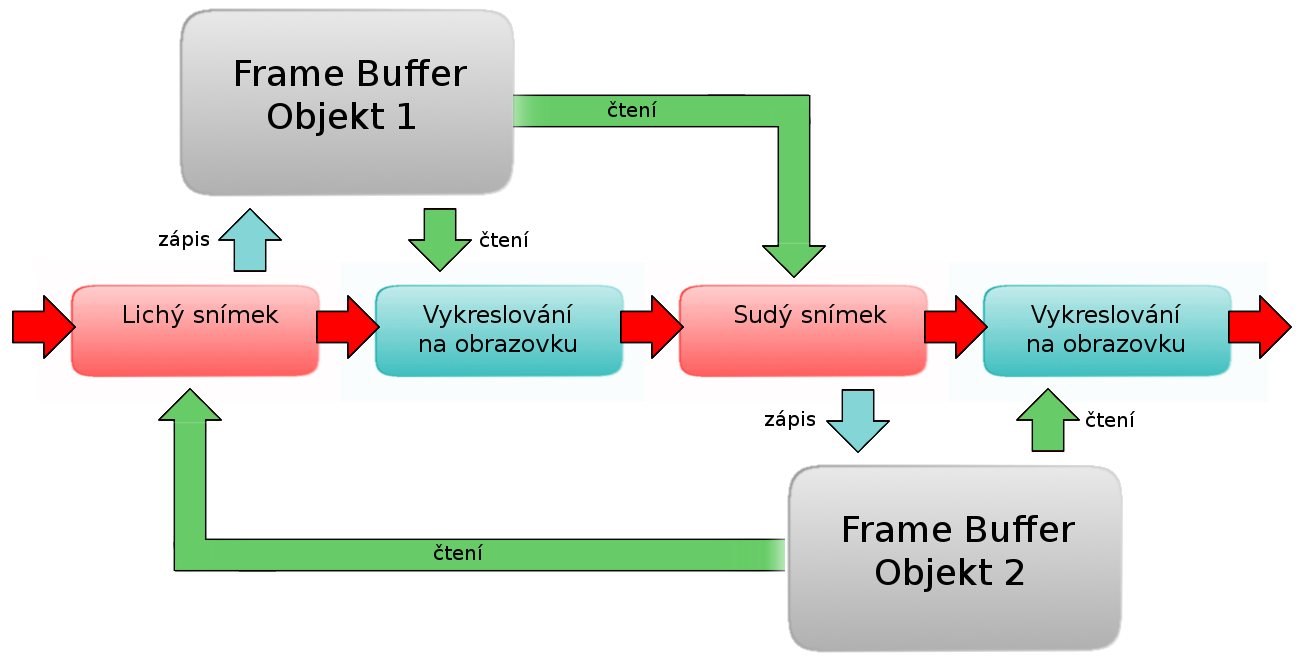
\includegraphics[width=140mm]{figures/screenspace.png}
\caption{Vykreslovací řetězec screen-space přístupu}
\end{figure}
\end{center}

\subsection{Rozměr textur na OpenGL ES 2.0}
Verze OpenGL ES 2.0 umožňuje používat obdélníkové textury pouze omezeně. Strana textury musí být o velikosti mocniny 2.
Pro vykreslování do textury, která bude výsledně umístěna na obrazovku je tedy nutné zvolit vyšší rozlišení. Např. u tabletu Google Nexus 7 2012 s rozlišením 1280x720 se zvolí textura 2048x1024. To znamená, že by se ve výsledku vykreslilo víc než 2x více pixelů než je potřeba.

Není ale nutné vykreslovat do celé textury, pomocí příkazu \textit{glViewport} se dá nastavit část textury, do které má OpenGL vykreslovat a nedojde tedy k plýtvání výkonem.

Dále je možné zvolit nižší rozlišení viewportu než je rozlišení displeje. Mobilní zařízení obvykle disponují obrovskou hustotou pixelů a pokud zařízení nebude stíhat vykreslovat scénu v plném rozlišení, lze vykreslovat v rozlišení menším. U počítačových 3D her se také setkáváme s možností změnit rozlišení, tam řeší změnu přímo hardware displeje nebo jeho ovladač.

\subsection{Motion-blur}
Jedním z efektů využívající screen-space přístup je motion-blur. Jedná efekt rozmáznutí obrazu rychlým pohybem. Motion-blur se používá ve většině závodních simulátorů, rozostření pohybem dodává dojem rychlosti.
\lstset{language=GLSL} 
\begin{lstlisting}[caption=Motion blur fragment shader dle rychlosti vozidla]
uniform sampler2D color_texture, pFrm;
uniform float res, speed;
varying vec2 v_Coords;

void main() {
	//apply color texture
	gl_FragColor = texture2D(color_texture, v_Coords); 

	//apply motion blur
	gl_FragColor *= (1.0 - speed);
	gl_FragColor += speed * texture2D(pFrm, gl_FragCoord.xy * res);
}
\end{lstlisting}

$Speed$ je rychlost vozidla od 0 do 1, $pFrm$ je textura předchozího snímku a $res$ je\linebreak 1 / \textit{plné rozlišení textury} (pro jednoduchost je použitý čtvercový rozměr textury).

Tento kód využívá screen-space informaci (texturu $pFrm$). Rozostření se projeví po několik snímků za sebou (efekt zůstává na obrazovce a postupně se utlumuje v závislosti na rychlosti vozdila). Nevýhodou je, že tento kód musí být vložen do každého shaderu vykreslující 3D model, aby motion-blur fungoval tak jak má.

\subsection{Odlesky}
Dále je možné ve screen-space řešit odlesky. Existuje obecný (složitý) postup jak tyto odlesky vypočítat, který by mobilní hardware nezvládl. Problém jsem rozdělil podle typu ploch. Vzhledem k tomu, že v simulátoru dochází pouze k rotaci pohledu podle osy y (rotace yaw), je možné řešit pro odlesky pro různé tvary povrchů zvlášť.

Abychom vytvořili odlesk povrchu vozovky optimálně, potřebovali bychom informaci\linebreak o hloubce scény. To by bylo opět výpočetně náročné, a proto jsem zvolil jednodušší postup. Odlesk funguje pouze pro jeden úhel pohledu mezi vozovkou a směrovým vektorem kamery.

Na úrovni přední řezné roviny kamery je horizont povrchu přesně v polovině obrazovky. Pokud budeme tedy mít normálu povrchu směřující kolmo nahoru, jsme schopni realizovat odlesk pomocí převrácení aktuální vykreslovací textury. Pro souřadnice aktuálně vykreslovaného fragmentu $[f_x, f_y, f_z]$ vypočteme souřadnice odlesku $r$ převrácením y hodnoty. Tím získáme odlesk na úrovni  přední řezné roviny.
\begin{center}
$r = [f_x, 1 - f_y]$
\end{center}
\newpage

S rostoucí vzdáleností od přední řezné roviny se lineárně posouvá horizont směrem vzhůru. Nalezením konstanty $a$ získáme souřadnice odlesku $r'$ pro kolmý povrch limitovaný úhlem pohledu kamery.
\begin{center}
$r' = [f_x, 1 - f_y + f_z \cdot a]$
\end{center}

Dále je potřeba podporovat i nekolmé povrchy. To se provede nalezením další konstanty $b$, která bude měnit lineární posun odlesku podle normály povrchu $\vec{n}$. Tím získáme souřadnice odlesku $r''$ limitované pouze úhlem pohledu kamery.
\begin{center}
$r'' = [f_x, 1 - f_y + f_z \cdot a + f_z \cdot (1 - n_y) \cdot b]$
\end{center}

\begin{center}
\begin{figure}[h!]
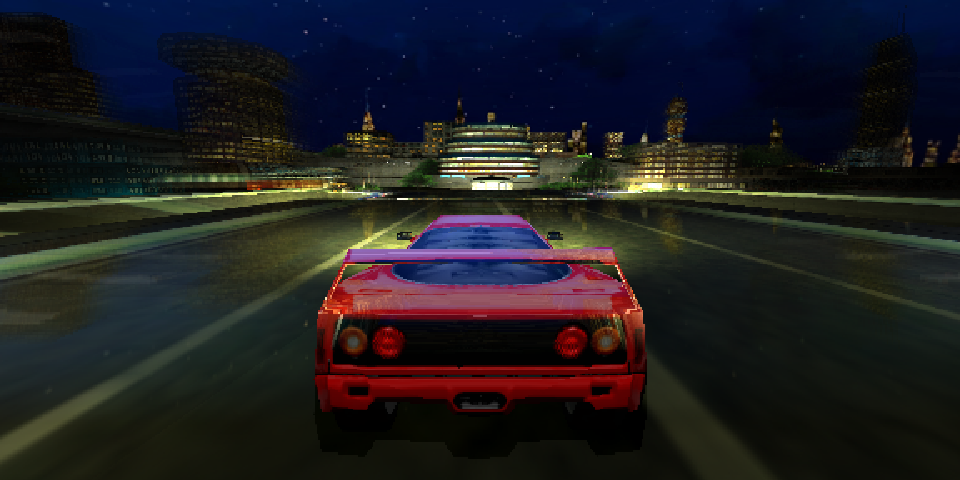
\includegraphics[width=140mm]{figures/reflect-horizont.png}
\caption{Odlesky na povrchu vozovky}
\end{figure}
\end{center}

Pro můj zvolený pohled jsem zvolil konstanty $a = 0.1; b = 2$. Odlesk vizuálně odpovídá a vykresluje se velice rychle. Problém je při nízké snímkovací frekvenci, kdy dochází k posunu odlesku (jak je vidět na obrázku 5.10). Posun není nijak výrazný, ale pokud se na něj soustředíme, vidíme jej. Dále při mísení efektů odlesků s motion-blurem dochází k rozmazání odlesku více než původního obrazu. Motion-blur je pro odlesky dvojnásobný, protože se aplikuje jak na původní objekt, tak na zrcadlový povrch.
\bigskip

U vozidel by se optimálně měl odlesk řešit pomocí víceprůchodového algoritmu za využití cube mapování. Vzhledem k tomu, že potřebuji maximální možný výkon a Android zařízení mají typicky malý displej, použil jsem jednodušší variantu.

Souřadnice odlesku $r$ u vozidel se provádí pouze podle normály. Pro výpočet pozice odraženého obrazu se vezme střed vozidla $s$ v souřadnicích kamery a přičte se k němu normála $\vec{n}$ vynásobena určitým faktorem $f$ (toto platí pouze pro vozidla, které uživatel ovládá).
\begin{center}
$r = [s_x + n_x \cdot f, s_y + n_y \cdot f]$
\end{center}

\begin{center}
\begin{figure}[h!]
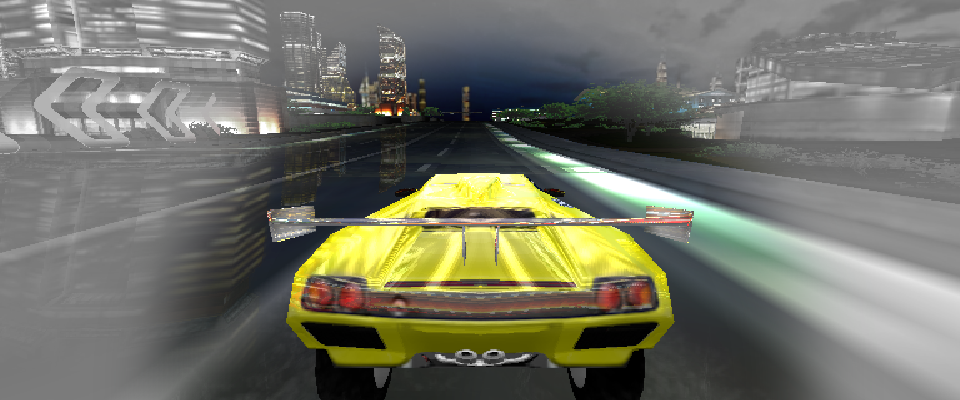
\includegraphics[width=150mm]{figures/reflect-car.png}
\caption{Ukázka výsledných odlesků na vozidle, vlevo bez odlesků, vpravo s odlesky}
\end{figure}
\end{center}

\subsection{Statické osvětlení a dynamické objekty}

Pokud máme ve scéně předpočtené stíny, je vhodné tyto statické stíny aplikovat\linebreak i na dynamické objekty. V případě vozidla lze přečíst intenzitu osvětlení z některých bodů na silnici pod vozidlem. Intenzitu osvětlení lze jednoduše ukládat do alfa kanálu textury,\linebreak ve které se nachází aktuální scéna.

Výpočet pozice bodu na obrazovce se provádí na CPU. Fyzikální engine vrací pozici středu vozidla $\vec{p}$, tu lze vynásobit maticí $MVP$ a po perspektivním dělením získáme pozici vozidla na obrazovce označenou jako $sp$. 
\begin{center}
$s = MVP \cdot \vec{p}$\\
$sp = s / s_w$
\end{center}
Pozice je v rozmezí $<-1, 1>$. Pro čtení z textury je třeba pozici přepočítat do rozmezí $<0, 1>$.
\begin{center}
$sp' = sp \cdot 0.5 + 0.5$
\end{center}

Tím jsme získali pozici vozidla, pokud chceme pozici pod vozidlem, musíme vypočítat pozici o něco níž. Úroveň posunu označím jako $a$. Velikost posunu je dále závislá na vzdálenosti vozidla od kamery. Vzdálenost je uložená v proměnné $s_z$.
\begin{center}
$sp''_x = sp'_x$\\
$sp''_y = sp'_y - a / s_z$
\end{center}

Tím jsme získali pozici texelu nesoucí informaci o intenzitě osvětlení. Vzniká zde ale problém s barevným světlem. Jsou zde dvě možnosti řešení. Prvním je přidání další textury, ve kterém by byla barevná intenzita světla (tím by došlo ke zvýšení náročnosti na hardware a ke zvýšení paměťové náročnosti). Druhým možným řešením je omezit barevná světla\linebreak do nějaké sytosti (pokud se slabě zabarvené světlo aplikuje jako bílé, není to tolik rušivé).

Dalším problémem je, že dynamické objekty (tedy vozidla) by měly zastínit statický model. Tento problém lze řešit opět pomocí screen-space přístupu. Ve screen-space textuře si můžeme označit texely (odpovídajících pixelům na obrazovce), na kterých je vykreslené vozidlo. V době vykreslování vozovky se vždy díváme o několik texelů výše, než je aktuální vykreslovaný fragment, a pokud je texel označen, ztmavíme aktuálně vykreslovaný fragment. Důležitou poznámkou je, že texely kol vozidla se neoznačují (tím by vznikal chybný stín).

Stín je kvalitou srovnatelný s projektivním stínem. Bylo by možné zjišťovat pozice světel, aby vznikl měkký stín, ale tím by se simulátor značně zpomalil. Při rychlém otáčení lze zpozorovat chybu, která vzniká kvůli použitému screen-space přístupu. V noční scéně to moc není vidět, nicméně ve světlých scénách by to mohlo být značně rušivé.

\begin{center}
\begin{figure}[h]
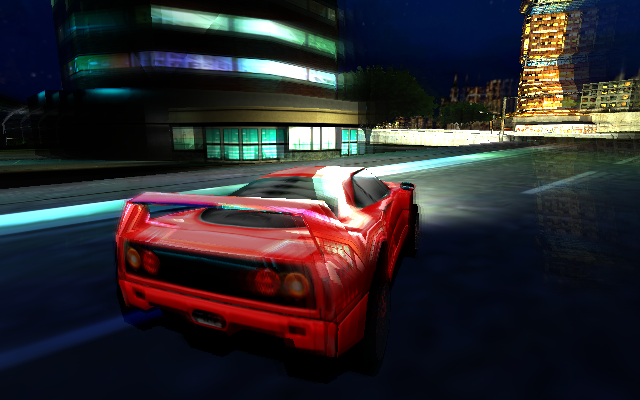
\includegraphics[width=120mm]{figures/nearshadow.png}
\caption{Vržený stín vozidla}
\end{figure}
\end{center}

\subsection{Světla vozidel}

Dle předběžných měření jsem zjistil, že na mobilních zařízeních lze za běhu počítat jedno až dvě světla (bez výpočtu zastínění zdroje světla). U vozidla ovládané hráčem není potřeba řešit viditelnost světla, prakticky zde nedochází k situacím, že by světlo osvětlovalo neviditelné objekty (je to z důvodu těsné vazby světla hráčova vozidla a kamery).

U ostatních vozidel je třeba osvětlení zjednodušit, aby to mobilní hardware zvládal. Zvolil jsem metodu vykreslování poloprůhledných kuželů do scény, k tomu je použita OpenGL funkce blending, která umožňuje kreslit objekty s částečnou průhledností. Je zde počítán útlum světla stejně jako u standardních světel.

%*****************************************************************************
\chapter{Testování}
Testování aplikace probíhalo na smartphonu, tabletu a laptopu, které jsou blíže popsány v tabulce 5.1. Zařízení byla během testování plně nabita, byla připojena ke zdroji napájení a byly vypnuty volby úspory energie. Veškeré testy byly prováděny za stejných podmínek.

\begin{table}[h!]
\begin{center}
\begin{tabular}{|p{29mm}|p{38mm}|p{38mm}|p{38mm}|}
\hline
& \textbf{Samsung Galaxy S3 mini (mobil)} & \textbf{Google Nexus 7 2012 (tablet)} & \textbf{Acer TravelMate P253-e (laptop)} \\
\hline
Procesor & NovaThor U8500 & ARM Cortex-A9 & Intel Pentium 2020M \\ \hline
Počet jader & 2 & 4+1* & 2 \\ \hline
Frekvence CPU & 1.0GHz & 1.3GHz & 2.4GHz \\ \hline
Operační paměť & 1GB & 1GB & 4GB DDR3 1066 MHz \\ \hline
Grafická karta & ARM Mali-400 MP & Nvidia Tegra 3 & Intel HD 4000 \\ \hline
Rozlišení displeje & 800x480 & 1280x800 & 1366x768 \\ \hline
Operační systém & Android 4.1.2 & Android 4.4.2 & Kubuntu 14.04 32bit \\ \hline
\end{tabular}
\caption{Parametry zařízení, na kterých jsem projekt testoval. U Android zařízení nebyly nalezeny bližší informace o typu operační paměti}
*tablet má extra procesor pro nižší spotřebu během nečinnosti
\end{center}
\end{table}
\newpage

\section{Generování map osvětlení}
Před testováním samotné aplikace jsem provedl testování generátoru map osvětlení. Testování bylo prováděno na laptopu Acer TravelMate P253-e jehož parametry jsou uvedeny na předchozí straně.

\paragraph{Bodové zdroje světla}\ \ \\

Při vykreslování bodových světel jsem testoval techniky generování map osvětlení. Techniky se nedají srovnat na nižší instanci, protože se principiálně odlišují. Provedl jsem tedy měření doby trvání celkového výpočtu pro malou instanci dat - scéna s 106ti bodovými světly.
\begin{table}[h!]
\begin{center}
\begin{tabular}{|p{50mm}|c|}
\hline
\textbf{Generátor map osvětlení} & \textbf{Čas vykreslování} \\
\hline
rasterizační bez PCF & 2.25min\\ \hline
rasterizační s PCF8x8 & 19.267min\\ \hline
vrhání paprsku & 28.176min\\ \hline
\end{tabular}
\caption{Vykreslování 106 bodových zdrojů světla pomocí OpenGL a pomocí raycastingu}
\end{center}
\end{table}

Rasterizační technika (za využití OpenGL) dosahuje výsledku o poznání rychleji. Pravděpodobně by výsledek nebyl tak rychlý bez hardwarové akcelerace a paralizace výpočtu, která u techniky vrhání paprsku není.

\paragraph{Plošné zdroje světla}\ \ \\

V případě plošných zdrojů je vhodnější použití techniky vrhání paprsků. Paprsky bývají téměř rovnoběžné a lze tedy jedním testem detekovat průsečík více paprsků najednou (za využití mailboxingu). V níže uvedeném testu se ukázala efektivita filtrování paprsků, u kterých je jejich délka delší než vzdálenost, ve které je světlo zcela utlumeno.
\begin{table}[h!]
\begin{center}
\begin{tabular}{|p{80mm}|c|c|}
\hline
\textbf{Nastavení} & \textbf{MegaRays/s} & \textbf{Všechny mapy osv.} \\
\hline
kvadratický útlum 0.2 & 657.89 & 10.276s\\ \hline
kvadratický útlum 0.1 & 348.43 & 19.483s\\ \hline
kvadratický útlum 0.05 & 183.82 & 36.875s\\ \hline
neseřazené trojúhelníky & 7.06 & 960.546s\\ \hline
neseřazené trojúhelníky, spot efekt 0.5 & 0.53 & 12874.661s\\ \hline
\end{tabular}
\caption{Vykreslování několika plošných zdrojů světel navzorkovaných na 202 bodových světel, neseřazené trojúhelníky znamená, že paprsky byly testovány neoptimálním pořadí }
\end{center}
\end{table}
\newpage

V dalším testu jsem zvolil větší instanci dat - 150306 bodových světel. Hrubým odhadem by vypočtení této instance pomocí rasterizace trvalo cca 50 hodin (100 světel/2 minuty, což je přímou úměrou 150000 světel/3000 minut). Vrhání paprsků pro tuto instanci dopadlo mnohem lépe.

\begin{table}[h!]
\begin{center}
\begin{tabular}{|p{80mm}|c|c|}
\hline
\textbf{Nastavení} & \textbf{MegaRays/s} & \textbf{Všechny mapy osv.} \\
\hline
kvadratický útlum 0.2 & 1149.43 & 1.219h\\ \hline
kvadratický útlum 0.2 dupl.test & 1063.83 & 1.322h\\ \hline
kvadratický útlum 0.1 & 584.80 & 2.398h\\ \hline
kvadratický útlum 0.1 dupl.test & 531.91 & 2.635h\\ \hline
kvadratický útlum 0.05 & 294.99 & 4.746h\\ \hline
kvadratický útlum 0.05 dupl.test & 268.09 & 5.222h\\ \hline
bez detekování dosahu & 68.12 & 20.561h\\ \hline
\end{tabular}
\caption{Vykreslování všech plošných zdrojů světel navzorkovaných na 150306 bodových světel, duplicitní test znamená filtrování trojúhelníků, které byly pro daný paprsky již testovány }
\end{center}
\end{table}

\begin{figure}[h!]
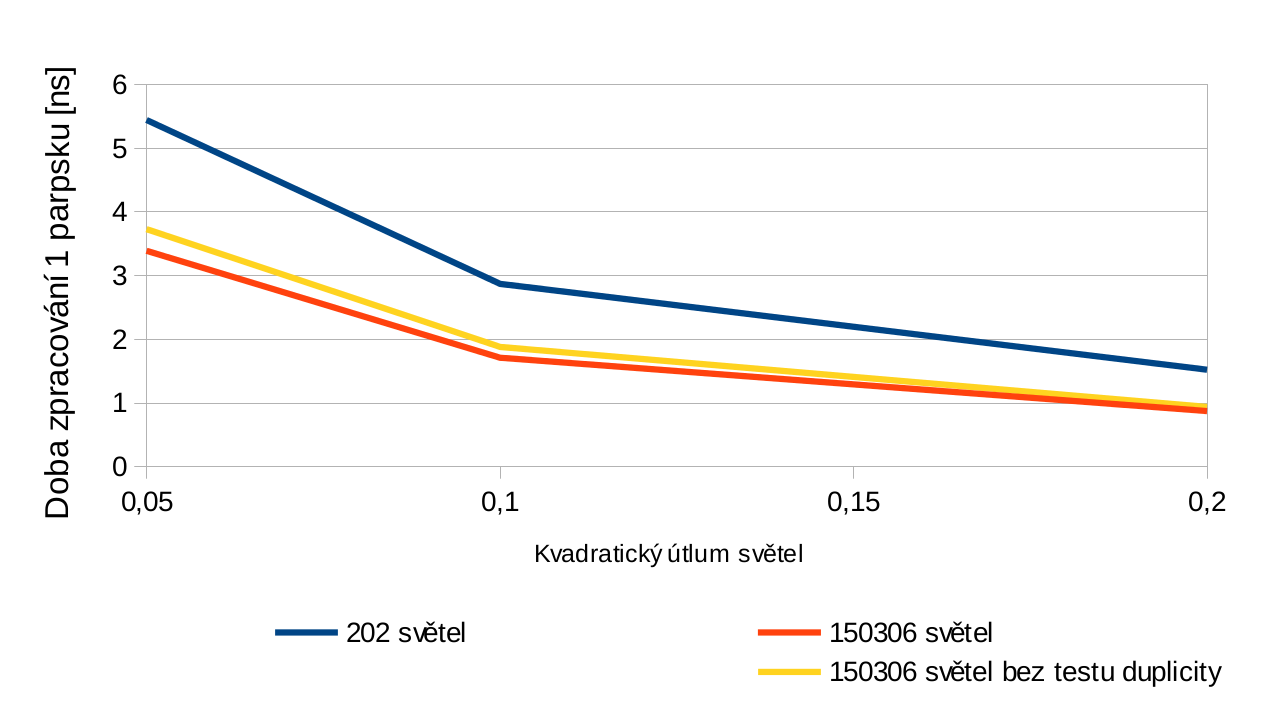
\includegraphics[width=150mm]{figures/graf3.png}
\caption{Závislost rychlosti zpracování paprsku na dosahu zdrojů světel, testování různě osvětlených scén}
\end{figure}
\newpage

\paragraph{Paměťová náročnost generátoru map osvětlení}\ \ \\

Paměťová náročnost byla naměřena pomocí Linuxového měřiče paměti KSysGuard. Generátor map osvětlení byl za běhu několikrát pozastaven a bylo provedeno měření celkového využití paměti generátorem. Z naměřených informací poté byly vypočteny hodnoty pro jednotlivé data. K vykreslení 8 map osvětlení o rozlišení 2048x2048 bylo použito celkem 1.94GB operační paměti.
\begin{figure}[h!]
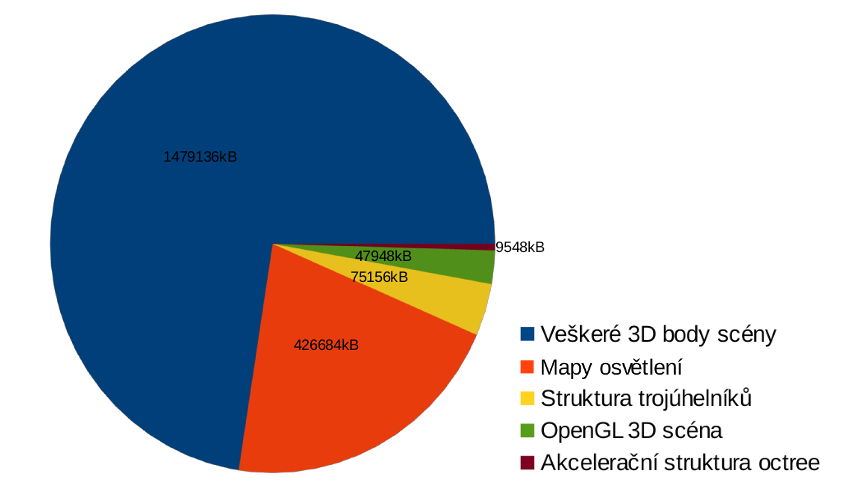
\includegraphics[width=100mm]{figures/lmgen-mem-usage.png}
\caption{Paměťová náročnost generátoru map osvětlení využívající vrhání paprsků. Scénou byl 3D model nočního města složený z přibližně 40000 trojúhelníků, vykreslováno bylo 8 map osvětlení o rozlišení 2048x2048 }
\end{figure}

Mapy osvětlení využívají více paměti než v testovací aplikaci, protože kromě informace o barvě uchovávají indexy jednotlivých trojúhelníků a barycentrické souřadnice pro každý texel. Struktura trojúhelníků zabírá také více paměti, protože uchovává pomocné informace pro rychlejší zpracování jako je například seznam 3D bodů (navzorkovaných podle rozlišení mapy osvětlení), které trojúhelník tvoří. 

3D body trojúhelníků obsahují interpolované hodnoty, které využijí o řád více paměti než samotné trojúhelníky. Interpolované hodnoty by bylo možné počítat za běhu aplikace, ale to by způsobilo značné zpomalení generování map osvětlení.

\section{Testovací aplikace - simulátor}

U testovací aplikace jsem nejdříve testoval rychlost vykreslování stejné sekvence snímků na testovaných zařízeních bez aktualizování map osvětlení. Sekvence byla dlouhá 1 vteřinu a u každé konfigurace bylo provedeno cca 10 měření. V tabulce 6.5 je vždy uvedena nejlepší hodnota měření. Testovací aplikace disponuje omezovačem snímkovací frekvence, která je nastavena na 20FPS. U Android verze je oproti verzi pro Linux použita paralelizace výpočtů na CPU. Vlákna na CPU musí být synchronizována, a proto Android zařízení nedosahují horního limitu snímkovací frekvence.
\newpage

\begin{table}[h!]
\begin{center}
\begin{tabular}{||p{25mm}||c|c||c|c||c|c||}
\hline
Poměr & \multicolumn{2}{c||}{\textbf{Samsung Galaxy}}
& \multicolumn{2}{c||}{\textbf{Google Nexus 7}}
& \multicolumn{2}{c||}{\textbf{Acer TravelMate}} \\
rozlišení proti & \multicolumn{2}{c||}{\textbf{S3 mini (mobil)}}
& \multicolumn{2}{c||}{\textbf{2012 (tablet)}}
& \multicolumn{2}{c||}{\textbf{P253-e (laptop)}} \\
nativnímu & FPS & snímek [ms] & FPS & snímek [ms] & FPS & snímek [ms] \\
\hline
0.4x (poor)   & 18 & 53.661 & \textbf{18} & \textbf{28.970} & \textbf{20} & \textbf{3.965} \\ \hline
0.5x (low)    & 17 & 50.898 & 18 & 37.547 & 20 & 4.010 \\ \hline
0.6x (normal) & 14 & 67.660 & 18 & 42.598 & 20 & 3.957 \\ \hline
0.8x (high)   & 11 & 90.710 & 17 & 60.187 & 20 & 4.432 \\ \hline
1.0x (ultra)  & \textbf{10} & \textbf{99.546} & 13 & 80.480 & 20 & 4.422 \\ \hline
\end{tabular}
\caption{Závislost rychlosti vykreslování scény na zařízení a úrovni rozlišení oproti nativnímu(v závorce je uvedena konfigurace v nastavení simulátoru). Tučně jsou zvýrazněny konfigurace, u kterých je přibližně stejný počet vykreslovaných pixelů}
\end{center}
\end{table}

Z výsledku je patrně vidět výkonový rozdíl mezi laptopem proti tabletu a mobilu. Laptop je přibližně 10x rychlejší než tablet při použití srovnatelného rozlišení.

\begin{figure}[h!]
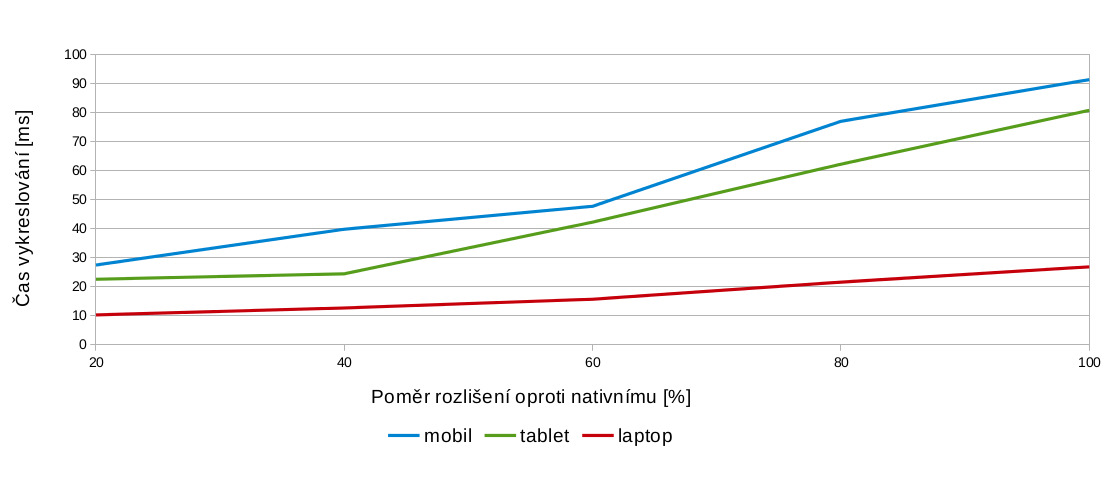
\includegraphics[width=150mm]{figures/graf2.png}
\caption{Závislost rychlosti vykreslování scény na zařízení a poměru rozlišení oproti nativnímu}
\end{figure}

Dále jsem měřil rychlost aktualizace 13ti dynamických světel najednou. Měření bylo provedeno na všech testovacích zařízeních pro dvě různé rozlišení map osvětlení. Ve všech případech se světla rozkládala na osmi mapách osvětlení.

\begin{table}[h!]
\begin{center}
\begin{tabular}{|p{35mm}|p{35mm}|p{35mm}|p{35mm}|}
\hline
& \textbf{Samsung Galaxy S3 mini (mobil)} & \textbf{Google Nexus 7 2012 (tablet)} & \textbf{Acer TravelMate P253-e (laptop)} \\
\hline
1024x1024 & 41.712 & 9.776 & 1.797 \\ \hline
2048x2048 & 132.411 & 10.836 & 1.790 \\ \hline
\end{tabular}
\caption{Závislost rychlosti aktualizace map osvětlení na platformě a rozlišení textur map osvětlení při vizuálních detailech normal(poměr 0.6x oproti nativnímu rozlišení)}
\end{center}
\end{table}

Výrazná závislost rychlosti aktualizace map se projevila pouze na mobilním telefonu,\linebreak u kterého je aktualizace celkově nejpomalejší. 

\paragraph{Paměťová náročnost testovací aplikace}\ \ \\

Paměťová náročnost byla opět naměřena pomocí Linuxového měřiče paměti KSysGuard. Testovací aplikace byla přerušována během načítání dat a z naměřených hodnot byla vypočtená paměť pro jednotlivé komponenty. Scéna využívající 8 map osvětlení o rozlišení 1024x1024 využívá 80.64MB operační paměti.

\begin{figure}[h!]
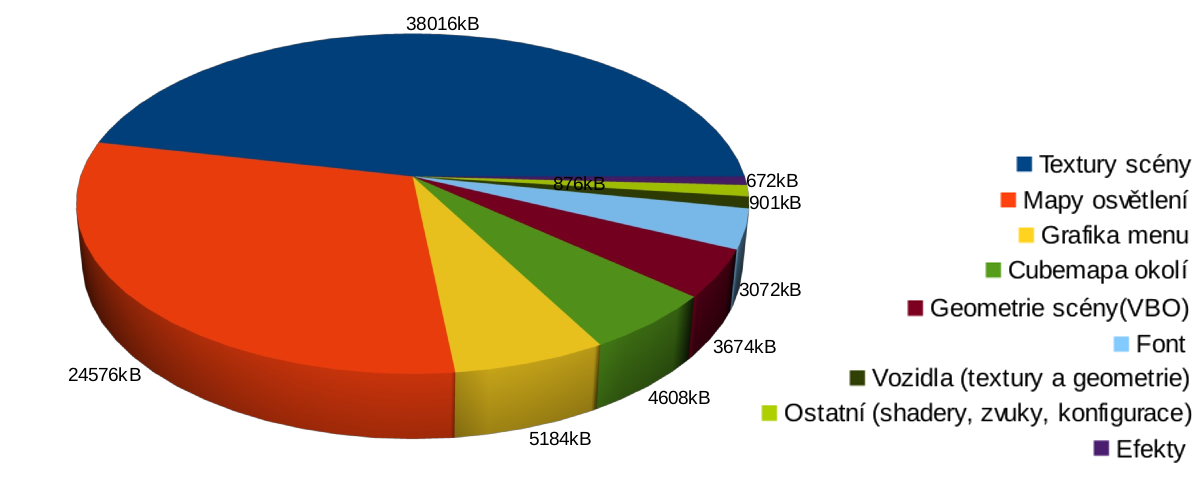
\includegraphics[width=120mm]{figures/sim-mem-usage.png}
\caption{Paměťová náročnost simulátoru se scénou 3D modelu nočního města složeného z přibližně 40000 trojúhelníků }
\end{figure}

V posledním testu jsem testoval kompatibilitu s dalšími zařízeními, v testu uspěl tablet Google Nexus 7 2013, Samsung Galaxy S4 a smartTV za použití Android set-top-boxu eGreat U8. V případě set-top-boxu bylo nutné ještě implementovat ovládání hardwarovými tlačítky. Další zařízení nebyla testována. Uvedená zařízení byla testována pouze na kompatibilitu, byla zapůjčena pouze na několik desítek minut.

%*****************************************************************************
\chapter{Závěr}

Úspěšně jsem realizoval generování map osvětlení pomocí vrhání paprsku a rasterizace. Generování map osvětlení pomocí vrhání paprsků umožňuje zpracování plošných zdrojů světel definovaných pomocí osvětlovacích textur. Je podporováno dynamické aktualizování map osvětlení pomocí záplat, které jsou komprimovány ve vektorové podobě v paměti grafické karty.

Realizoval jsem testovací aplikaci, která mapy osvětlení využívá a nad rámec zadání jsem aplikoval statické osvětlení na dynamické objekty. Vylepšil jsem výsledek aplikováním odlesků a motion-blur. Výsledek jsem úspěšně otestoval na několika zařízeních. Podle měření je testovací aplikace poměrně náročná na výkon, nicméně mobilní zařízení střední a vyšší třídy s aplikací nemají problém.

Vzniklá aplikace sice není po grafické stránce schopna konkurovat komerčním simulátorům na platformě Android. Nicméně disponuje několika grafickými technikami, které mnoho komerčních simulátorů postrádá. Předzpracované osvětlení dodává scéně lepší vzhled a povedlo se dokonce aplikovat předzpracované osvětlení i na dynamické objekty.

Práci do budoucna hodlám dále vyvíjet. Chci se soustředit hlavně na další možnosti optimalizace, jako je například ořez scény pohledovým jehlanem, použití techniky Level-of-detail a dynamické načítání scény.

%*****************************************************************************
% Seznam literatury je v samostatnem souboru reference.bib. Ten
% upravte dle vlastnich potreb, potom zpracujte (a do textu
% zapracujte) pomoci prikazu bibtex a nasledne pdflatex (nebo
% latex). Druhy z nich alespon 2x, aby se poresily odkazy.

%\bibliographystyle{abbrv}
\bibliographystyle{plain}
%\bibliographystyle{psc}
{
%JZ: 11.12.2008 Kdo chce mit v techto ukazkovych odkazech take odkaz na CSTeX:
%\def\CS{$\cal C\kern-0.1667em\lower.5ex\hbox{$\cal S$}\kern-0.075em $}
\raggedright
\bibliography{reference}
}

% M. Dušek radi:
%\bibliographystyle{alpha}
% kdy citace ma tvar [AutorRok] (napriklad [Cook97]). Sice to asi neni  podle ceske normy (BTW BibTeX stejne neodpovida ceske norme), ale je to nejprehlednejsi.
% 3.5.2009 JZ polemizuje: BibTeX neobvinujte, napiste a poskytnete nam styl (.bst) splnujici citacni normu CSN/ISO.

%*****************************************************************************
%*****************************************************************************
\appendix

\chapter{Seznam použitých zkratek}
\begin{itemize}
\item 3D (Three-dimensional) - trojrozměrné
\item API (Application Interface) - aplikační rozhraní
\item CPU (Central Processing Unit) - centrální výpočetní jednotka - procesor
\item FBO (Fragment Buffer Object) - buffer určený pro vykreslování scény
\item GLSL (OpenGL Shading Language) - jazyk pracující s grafickou kartou k výpočtu stínování
\item GPU (Graphics processing unit) - grafická výpočetní jednotka - grafická karta
\item UML (Unified Modeling Language) - vizuální jazyk pro modelování softwaru
\item VBO (Vertex Buffer Object) - geometrie uložená na GPU
\end{itemize}

\chapter{Obsah přiloženého CD}

\begin{center}
\begin{tabular}{|p{50mm}|p{100mm}|}
\hline
\textbf{Položka} & \textbf{Popis}\\
\hline
bin/android & několik verzí testovací aplikace pro Android\\
\hline
bin/linux/assets & data testovací aplikace\\
\hline
bin/linux/lmgenerator & generátory map osvětlení\\
\hline
bin/linux/objConverter.jar & konvertor modelů\\
\hline
bin/linux/testapp & spustitelná verze testovací aplikace pro Linux\\
\hline
doc/latex & editovatelná dokumentace simulátoru\\
\hline
doc/text.pdf & dokumentace simulátoru\\
\hline
src/lmgenerator & zdrojové kódy generátorů map osvětlení\\
\hline
src/objconverter & zdrojové kódy konvertoru modelů\\
\hline
src/testapp & zdrojové kódy testovací aplikace\\
\hline
src/support & knihovny potřebné ke zkompilování simulátoru\\
\hline
install.txt & návod k instalaci\\
\hline
readme.txt & informace potřebné k používání\\
\hline
video.mp4 & ukázkové video testovací aplikace\\
\hline
\end{tabular}
\end{center}

\chapter{Uživatelská příručka}

\section{Generování map osvětlení}
Nejdříve třeba nadefinovat světelné zdroje 3D modelu. Bodové zdroje světla se definují pomocí 3D hran. Každé světlo se skládá z jedné hrany (zdroje světla a směru). Každá skupina světel musí být samostatný objekt. Plošné zdroje světla se definují pomocí osvětlovacích textur (viz kapitola 5.1.1). Osvětlovací textury musí být vytvořeny pro každou texturu 3D scény, musí být uloženy ve stejné cestě a mít místo přípony \textbf{png}, příponu \textbf{png-map}.

Aby bylo možné generovat mapy osvětlení je nutné mít 3D scénu ve formátu O4S. O4S formát modely se vytvoří konvertováním scény z formátu OBJ pomocí příkazu
\begin{center}
java -jar objConverter $<model>$.obj $<cesta$ $exportu>$/scene.o4s
\end{center}

Dále je třeba definovat konfiguraci generátoru map osvětlení pomocí souboru \textbf{lights.ini}.

\begin{lstlisting}[caption=Konfigurace generátoru map osvětlení]
CONFIG
//uhel orezu plosneho zdroje svetla
area_light_cutoff 90
//kvadraticky utlum plosneho zdroje svetla
area_light_att 0.2
//intenzita plosneho zdroje svetla
area_light_intensity 10
//tolerance pro rozdelovani trojuhelniku
interpolation_tolerancy 32
//rozliseni mapy osvetleni
lightmap_size 2048
//vykreslovani plosnych zdroju svetla(1=zapnuto, 0=vypnuto)
render_area_lights 1
//vykreslovani zaplat map osvetleni(1=zapnuto, 0=vypnuto)
render_dynamic_lights 1
//vykreslovani mapt osvetleni(1=zapnuto, 0=vypnuto)
render_lightmap 1
//scena pro generovani map - cesta k 3D modelu je v config/resources.txt
render_scene RACE2
END
\end{lstlisting}

Nakonec je potřeba definovat parametry jednotlivých skupin světel a po té již lze spustit generátor map osvětlení.
\begin{lstlisting}[caption=Konfigurace světla pro generátor map osvětlení]
LIGHT0
//shader pro vykresleni mapy osvetleni - pouze rasterizacni generator map
shader lightmap_spot
//informace, ze svetlo ma byt dynamicke(1=zapnuto, 0=vypnuto)
blink 1
//barva svetla, cervena slozka
R 4.0
//barva svetla, zelena slozka
G 4.0
//barva svetla, modra slozka
B 2.0
//orez reflektoru ve stupnich - zaporne cislo vykresli bodove svetlo
cut 60
//ignorovani blizkych objektu - pouze rasterizacni generator map
near 3
//spot efekt svetla
spot 0.5
//konstantni utlum svetla
att0 0.01
//linearni utlum svetla
att1 0.02
//kvadraticky utlum svetla
att2 0.05
END
\end{lstlisting}

Světla jsou indexována podle pozice objektu v modelu (indexováno od nuly, objekty neobsahující hrany jsou ignorovány).

Doporučuji použít generátor map osvětlení využívající vrhání paprsků (LMGenerator), rasterizační generátor (GLLMGenerator) nepodporuje plošné zdroje světel a dynamická světla.

\section{Testovací aplikace}
Testovací aplikace vyžaduje minimálně jednojádrový procesor o taktu 1GHz, 1GB RAM paměti, grafickou kartu s pamětí 64MB. Dále vyžaduje OpenGL ES 2.0 (nebo OpenGL 3.0) a GLSL 1.0. Binární soubor pro Android je kompatibilní s Android 4.0+.

\noindent Aplikace je ke stažení na adrese:\ \ \\
\textbf{http://play.google.com/store/apps/details?id=com.lvonasek.o4s}
\newpage

\subsection{Kompilování}

\paragraph{Linux}\ \ \\
Před kompilováním je potřeba mít nainstalované následující balíčky:\ \ \\
libbullet-dev freeglut3-dev libpng-dev qmake make\ \ \\
\ \ \\
Pokud máte 64bitový systém je potřeba nahradit v jni/open4speed.pro řádek\ \ \\
./fmodapi/libfmodex-4.44.08.so\ \ \\
řádkem\ \ \\
./fmodapi/libfmodex64-4.44.08.so\ \ \\
\ \ \\
Kompilování se spustí zadáním těchto příkazů do terminálu:\ \ \\
cd jni\ \ \\
qmake open4speed.pro\ \ \\
make

\paragraph{Android}\ \ \\
Součástí CD je několik verzí pro Android s různými konfiguracemi.\ \ \\
Pro kompilování je potřeba mít nainstalované následující software:\ \ \\
Android Studio, Android NDK(v případě potřeby kompilovat C++ kód)\ \ \\
\ \ \\
Kompilování C++ kódu:\ \ \\
cd jni\ \ \\
<cesta k Android NDK>/ndk-build\ \ \\
\ \ \\
Pro zbytek stačí otevřít projekt v Android Studiu a klepnout na Run

\subsection{Používání}
\paragraph{Menu}\ \ \\
\begin{itemize}
\item Start race - herní mód, je zde vytyčen okruh, závodí se s vozidly ovládané umělou inteligencí
\item Free ride - volná jízda po městě
\item Options - přejde do nabídky nastavení
\item Quit game - ukončí simulátor
\end{itemize}

\paragraph{Ovládání}\ \ \\
\begin{itemize}
\item šipky nahoru/dolu - plyn/brzda
\item šipky vlevo/vpravo - zatáčení
\item klávesa esc/zpět - pauza, menu pro restart závodu, ukončení závodu
\end{itemize}

\end{document}
